\clearpage

\section{Pipeline Recipes / CPL Plugins}
\label{sec:pipeline_recipes}

All functionality of the METIS pipeline is provided through \emph{recipes}, i.e.~CPL plugins that run in the contexts that ESO tools provide. This is in accordance with \cite{1618} and fulfills \REQ{METIS-6059} and \REQ{METIS-5945}.

Throughout this document we use the following color scheme for the
recipe workflows:
\begin{center}
  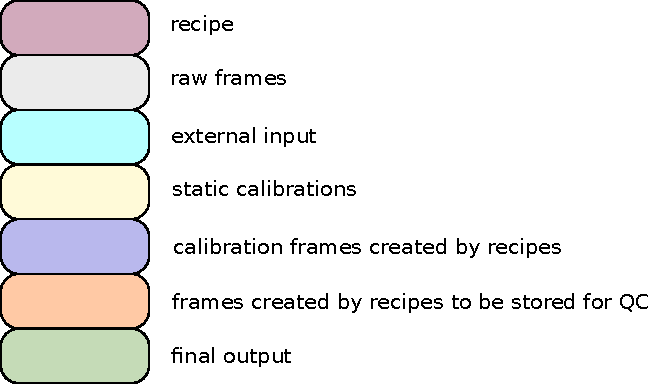
\includegraphics[width=0.3\textheight]{colour_legend}
\end{center}

%% Recipes_Detector.tex
%% Created:     Tue Apr  4 16:37:17 2017 by Koehler@I-Mac
%% Last change: 2020-09-04
%%
%% subsection for Detector Recipes
%%
%%%%%%%%%%%%%%%%%%%%%%%%%%%%%%%%%%%%%%%%%%%%%%%%%%%%%%%%%%%%%%%%%%%%%%%%%%%%%
\subsection{Detector calibration recipes}
\label{Sec:detector_calibration}

METIS will have three focal plane detector arrays:
\begin{itemize}
\item One $2\mathrm{k}\times 2\mathrm{k}$ HAWAII2RG detector used for
  LM-band imaging and slit spectroscopy.
\item One $2\mathrm{k}\times 2\mathrm{k}$ GeoSnap (Teledyne) detector
  used for N-band imaging and slit spectroscopy.
\item An array of four $2\mathrm{k}\times 2\mathrm{k}$ HAWAII2RG
  detectors used for LM-band integral-field spectroscopy.
\end{itemize}
This section lists recipes that calibrate detector characteristics
independent of a specific instrument mode. Where \FITS{_det} appears
in FITS keywords of input or product files, it is taken to mean
\FITS{_LM}, \FITS{_N} or \FITS{_IFU} according to the detector
array for which data are being processed.

\subsubsection{Detector linearity and gain determination recipe \REC{metis_det_lingain}}
\label{sssec:metis_det_lingain}
\label{rec:metis_det_lingain}
\label{rec:metisdetlingain}

The recipe \REC{metis_det_lingain} determines detector (non-)linearity and absolute detector
gain from a set of flat-field frames taken with the broad-band lamp
over a range of detector exposure times (DITs) and flux levels. The
recipe structure will be similar as for \CODE{detmon_ir_lg} % Not a \REC because it is not our recipe
\cite{detmon-manual}; however, further insight into detector behaviour
(in particular of GeoSnap) may necessitate development of more complex
procedures.

The linearity curve is given by the measured background level as a
function of exposure time for constant illumination. For each pixel
the coefficients of a polynomial fit (order TBD) will be recorded in a
coefficient cube, which can in turn be used to correct for
non-linearity in other recipes. Pixels whose coefficients differ
significantly from the majority of pixels will be marked as bad.

Detector gain is typically computed pixelwise as the slope of a linear
fit of the variance against the mean (or median) values over a set of
frames taken over a range of DITs and illumination levels.  For
mid-infrared detectors that suffer from \ac{ELFN}, e.g.\ the AQUARIUS
detector, this approach does not work.  The GeoSnap is not expected to
show \ac{ELFN}, hence gain determination is probably possible.

The set of calibration frames used for this recipes will include
exposures with WCU window closed (\CODE{LAMP OFF}), which will be used
as `dark' frames that captur thermal emission within the
instrument. This is subtracted from all other exposures in the
sequence.

This satisfies \REQ{METIS-5997}.

\newpage
\begin{recipedef}
  Name:                & \hyperref[rec:metis_det_lingain]{\REC{metis_det_lingain}}                                                             \\
  Purpose:             & determine non-linearity and gain of the detectors                                   \\
  Requirements:        & \REQ{METIS-5997}                                                                    \\
  Type:                & Calibration                                                                         \\
  Templates:           & \TPL{METIS_img_lm_cal_DetLin}                                                       \\
                       & \TPL{METIS_img_n_cal_DetLin}                                                        \\
                       & \TPL{METIS_ifu_cal_DetLin}                                                          \\
  Input data:          & \hyperref[dataitem:detlin_det_raw]{\RAW{DETLIN_det_RAW}}: (set of \FITS{FLAT,LAMP} frames taken with increasing DIT) \\
                       & \hyperref[dataitem:dark_internal_det_raw]{\RAW{DARK_INTERNAL_det_RAW}}: (set of internal darks taken at the start of the template) \\
  Matched keywords:    & Subsystem ID \TODO{TBD}                                                             \\
  Algorithm:           & Subtract instrument dark (\CODE{hdrl_imagelist_sub_image}).                         \\
                       & Compute mean and variance for each frame (\CODE{TBD}).                              \\
                       & Gain is determined as the slope of variance against mean (\hyperref[drl:metis_derive_gain]{\CODE{metis_derive_gain}}) \\
                       & Fit polynomial of value as a function of DIT and illumination level for each pixel (\hyperref[drl:metis_derive_nonlinearity]{\CODE{metis_derive_nonlinearity}}). \\
                       & Flag pixels with coefficients significantly different from the mean of all pixels. (\CODE{hdrl_bpm_fit_compute}) \\
  Output data:         & \hyperref[dataitem:gain_map_det]{\PROD{GAIN_MAP_det}}                                    \\
                       & \hyperref[dataitem:linearity_det]{\PROD{LINEARITY_det}}                                 \\
                       & \hyperref[dataitem:badpix_map_det]{\PROD{BADPIX_MAP_det}}                                \\
  Expected accuracies: & \TODO{TBD}                                                                          \\
  QC1 parameters:      & \hyperref[qc:qc_lin_gain_mean]{\QC{QC LIN GAIN MEAN}}                                    \\
                       & \hyperref[qc:qc_lin_gain_rms]{\QC{QC LIN GAIN RMS}}                                      \\
                       & \hyperref[qc:qc_lin_num_badpix]{\QC{QC LIN NUM BADPIX}}                                  \\
  hdrl functions:      & \CODE{hdrl_imagelist_sub_image}                                                     \\
                       & \CODE{hdrl_bpm_fit_compute}                                                         \\
\end{recipedef}

\begin{figure}[hb]
  \centering
  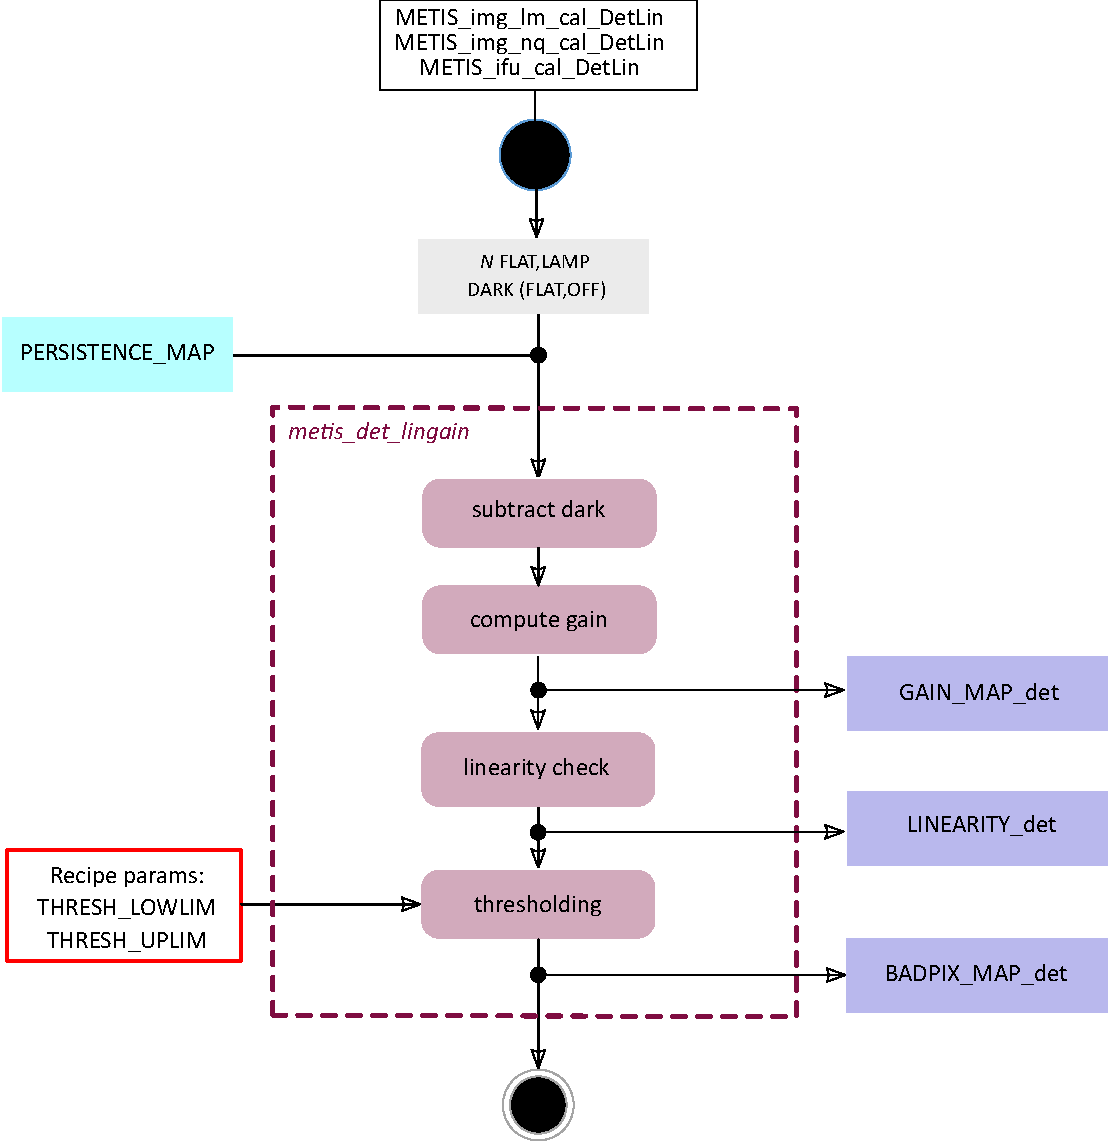
\includegraphics[width=0.65\textwidth]{metis_det_lingain}
  \caption[Recipe: \REC{metis_det_lingain}]{\REC{metis_det_lingain} --
    determination of linearity and gain of the detectors.}
  \label{Fig:rec_det_lingain}
\end{figure}


\clearpage

\subsubsection{Master dark recipe \REC{metis_det_dark}}
\label{sssec:metis_det_dark}
\label{rec:det_dark}
\label{rec:metis_det_dark}

Darks are taken in daytime for all science detectors
\cite{METIS-calibration_plan}. The data will be classified by detector
(e.g.~\FITS{DET.ID} and \FITS{DET.CHIP.ID}) and integration time
(\FITS{DET.DIT}).\footnote{The dark current is not expected to depend on the readout mode of the detectors. Should hardware tests reveal such a dependence, the recipe will be amended to classify on readout mode as well.} There will be ``METIS-dark''
(with the CLOSED position of the CFO-PP1 wheel) and ``Imager-dark''
(with the CLOSED position in the subsystem PP1), to be distinguished
by keyword \TBD. The former will be used for pipeline processing, the
latter for monitoring purposes.

Each set of raw dark frames is processed into a master dark. For the
IFU, both raw frames and master dark have four extensions
corresponding to the four detectors in the focal-plane array. The
recipe also produces bad pixel masks by identifying hot pixels whose
dark current differs significantly (by more than $\pm 5\sigma$) from
the average over the detector.

This fulfills \REQ{METIS-6063}.

\begin{recipedef}
  Name:                & \hyperref[rec:metis_det_dark]{\REC{metis_det_dark}}                                                        \\
  Purpose:             & determine the dark current of the detectors                                 \\
  Requirements:        & \REQ{METIS-6063}                                                            \\
  Type:                & Calibration                                                                 \\
  Templates:           & \TPL{METIS_gen_cal_dark}                                                    \\
  Input data:          & \hyperref[dataitem:linearity_det]{\STATCALIB{LINEARITY_det}}  \\
                       & \hyperref[dataitem:persistence_map]{\EXTCALIB{PERSISTENCE_MAP}}  \\
                       & \hyperref[dataitem:dark_det_raw]{\EXTCALIB{DARK_det_RAW}}  \\
  Parameters:          & Combination method (\texttt{median}, \texttt{mean},
                         \texttt{sigclip},\dots)                                                  \\
                       & Parameters for combination methods                                          \\
                       & Thresholds for deviant-pixel identification                                      \\
  Algorithm:           & Group files by detector and \texttt{DIT}, based on header keywords           \\
                       & Call function \DRL{metis_determine_dark} for each set of files\\
                       & Compute median or average of input frames to improve statistics.            \\  % separate routine, or part of determine dark
                       & call \DRL{metis_update_dark_mask} to flag deviant pixels \\
  Output data:         & \hyperref[dataitem:master_dark_det]{\PROD{MASTER_DARK_det}}                                                      \\
% The BPM_COLD_det and BPM_HOT_det do not seem to add value that BADPIX_MAP_det
% does not already provide. Furthermore, the COLD/HOT specific items are not
% otherwise used in the design, so it seems simpler to just remove them.
%                       & \hyperref[dataitem:bpm_cold_det]{\PROD{BPM_COLD_det}}                                                         \\
%                       & \hyperref[dataitem:bpm_hot_det]{\PROD{BPM_HOT_det}}                                                          \\
                       & \hyperref[dataitem:badpix_map_det]{\PROD{BADPIX_MAP_det}}                                                          \\
  Expected accuracies: & \TBD                                                                         \\
  QC1 parameters:      & \QC{QC DARK MEAN}                                                              \\
                       & \QC{QC DARK MEDIAN}                                                            \\
                       & \QC{QC DARK RMS}                                                               \\
                       & \QC{QC DARK NBADPIX}                                                             \\
                       & \QC{QC DARK NCOLDPIX}                                                               \\
                       & \QC{QC DARK NHOTPIX}                                                                \\
                       & (more \TBD)                                                                  \\
  hdrl functions:      & \CODE{hdrl_bpm_3d_compute}                                 \\
                       & \CODE{hdrl_imagelist_collapse}                             \\
\end{recipedef}

\begin{figure}[hb]
  \centering
  \includegraphics[width=0.5\textwidth]{figures/metis_det_dark_v0.83.pdf}  % RemarK. The original file: figures/metis_det_dark.pdf is still available
  \caption[Recipe: \REC{metis_det_dark}]{\REC{metis_det_dark} -- creation of master
    dark and bad pixel maps}
  \label{Fig:rec_det_dark}
\end{figure}

\clearpage

\subsubsection{Persistence map creation recipe \REC{metis_det_persistence}}
\label{sssec:metis_det_persistence}

Infrared detectors show persistent signal due to charges trapped on a
variety of timescales. The correction for a given science or
calibration exposure is built from a sequence of exposures preceding
the exposure in question. As these may include exposures taken for
another proprietary programme, the recipe is run by ESO on data taken
from the science archive and its products are again ingested into the
archive.

\begin{recipedef}\label{rec:metis_det_persistence}
  Name:                & \hyperref[rec:metis_det_persistence]{\REC{metis_det_persistence}}           \\
  Purpose:             & compute persistence correction maps        \\
  Requirements:        & \REQ{METIS-9145}                      \\
  Type:                & Calibration                           \\
  Templates:           & --                                    \\
  Parameters:          & \TBD                                  \\
  Algorithm:           & see hdrl functions:                   \\
  Output data:         & \hyperref[dataitem:persistence_map]{\PROD{PERSISTENCE_MAP}}                \\
  Expected accuracies: & \TBD                                  \\
  QC1 parameters:      & see hdrl functions:                   \\
  hdrl functions:      & \TBD (\CODE{hdrl_persistence_compute} \\
\end{recipedef}

\begin{figure}[hb]
  \centering
  \resizebox{0.6\textwidth}{0.1\textwidth}{\TODO{\fbox{Figure to be done}}}
  \caption[Recipe:
  \REC{metis_det_persistence}]{\REC{metis_det_persistence} -- creation
    of persistence correction frames.}
  \label{Fig:rec_det_persistence}
\end{figure}

%%%%%%%%%%%%%%%%%%%%%%%%%%%%%%%%%%%%%%%%%%%%%%%%%%%%%%%



%%% Local Variables:
%%% TeX-master: "METIS_DRLD"
%%% End:


\subsection{LM-band imaging}
\label{ssec:recipes_img_lm}

\subsubsection{LM-band imaging flatfield}
\label{lm_img_flatfield}
\label{rec:lm_img_flatfield}
\label{sssec:lm_img_flatfield}
\label{metis_lm_img_flat}
\label{rec:metis_lm_img_flat}
\label{sssec:metis_lm_img_flat}

The purpose of the flat-field calibration is to determine
pixel-to-pixel gain variations and large scale illumination variations
(due to inhomogeneities of optical elements in the telescope or
instrument). Calibration frames are obtained either during day time
using the black-body lamp of the \ac{WCU} (internal flats) or by taken
images of the twilight sky (twilight flats). Advantages and
disadvantages of the two types of flat are discussed in
\cite{METIS-calibration_plan}. Since the operational concept for
twilight flats needs to be refined during commissioning at the
telescope, the current recipe design is primarily valid for internal
flats.

This recipe creates a master flat for the HAWAII2RG detector (LM-band
imaging) from lamp or sky images matched by various setup parameters
as detailed below.  A set of internal flats includes a number of
exposures with \CODE{LAMP OFF}, which will be used for dark
subtraction. For twilight flats a master dark will be subtracted. The
master flat is obtained by the slope of a linear fit of the pixel
values against the illumination level of the exposures.

The quality control parameters give various statistics for each input
frame (mean, standard deviation, etc.), the standard deviation of the
normalised master flat and the number of bad pixels identified by the
recipe. If a bad-pixel map is provided on input, it is updated,
otherwise a new one is created.

\begin{recipedef}
  Name:                & \REC{metis_lm_img_flat}                                        \\
  Purpose:             & Create master flat field for the LM-band imaging detector.     \\
  Requirements:        & \REQ{METIS-6096}                                               \\
  Type:                & Calibration                                                    \\
  Templates:           & \TPL{METIS_img_lm_cal_InternalFlat}                            \\
                       & \TPL{METIS_img_lm_cal_TwilightFlat}                               \\
  Input data:          & Flat field images taken with lamp or sky.                      \\
                       & Master dark (for twilight flats)                               \\
                       & Bad pixel map                                                  \\
  Matched keywords:    & Detector ID                                                    \\
                       & Filter ID                                                      \\
                       & ADC ID                                                         \\
                       & Flat type (internal or twilight)                               \\
                       & possibly others (e.g.\ coronagraphic mask, \TBD)               \\
  Parameters:          & Combination method (\texttt{mean}, \texttt{median},
                         \texttt{sigclip}, \dots)                                       \\
                       & Parameters for combination methods                             \\
                         & Threshold(s) for deviant-pixel identification                  \\
 Algorithm:            & Call \DRL{metis_apply_persistance_correction} to apply the persistance correction \\
                         & For internal flats: call \REC{metis_det_dark} with \CODE{LAMP OFF} images to create dark frame. \\
 & Subtract internal dark or master dark from flat exposures.     \\
  & call \REC{metis_lm_img_flat} to fit slope of pixel values against illumination level. Frames
  with the same exposure time will be averaged.\\
                       & Compute median or average of input frames to improve statistics.\\
                       & Call \DRL{metis_update_lm_flat_mask} to flag deviant pixels. \\
  Output data:         & \hyperref[dataitem:master_img_flat_lm]{\PROD{MASTER_IMG_FLAT_LM}}                                      \\
                       & \hyperref[dataitem:badpix_map_lm]{\PROD{BADPIX_MAP_LM}}                                           \\
  Expected accuracies: & \TBD                                                           \\
  QC1 parameters:      & \QC{QC LM MASTERFLAT RMS}                                      \\
                       & \QC{QC LM FLAT NBADPIX}                                        \\
                       & \QC{QC LM FLAT MEAN ##}                                        \\
                       & \QC{QC LM FLAT RMS ##}                                         \\
  hdrl functions:      & \CODE{hdrl_bpm_fit_compute}                                    \\
                       & \CODE{hdrl_imagelist_collapse}                                 \\
                       & \CODE{hdrl_imagelist_sub_image}                                \\
\end{recipedef}

\begin{figure}[hb]
  \centering
  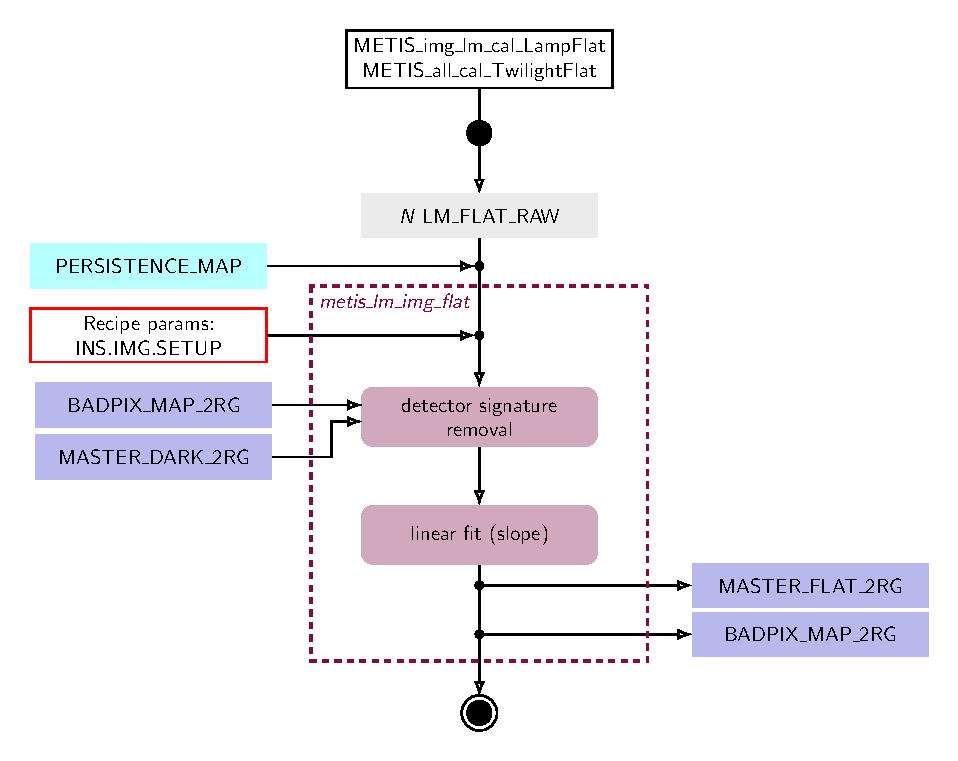
\includegraphics[width=0.6\textwidth]{metis_lm_img_flat}
  \caption[Recipe: \REC{metis_lm_img_flat}]{\REC{metis_lm_img_flat} --
    creation of \CODE{IMG_LM} master flatfield.\\ \TODO{Include averaging of
      frames at same illumination}}
  \label{fig:metis_lm_img_flat}
\end{figure}


\clearpage
\subsubsection{LM-band imaging basic reduction}
\label{lm_img_basic}
\label{rec:lm_img_basic}
\label{sssec:lm_img_basic}
\label{metis_lm_img_basic_reduce}
\label{rec:metis_lm_img_basic_reduce}
\label{sssec:metis_lm_img_basic_reduce}

\TODO{New recipe -- this may be too basic and could be joined with
  the background subtraction.}

This recipe performs the basic reduction of raw exposures from the
LM-band imager, i.e.\ dark subtraction, flat fielding and other removing
instrumental signals. It is used for both standard and science exposures.

Basic statistics of the images can be used to screen for saturation.

\TODO{This recipe should analyse the masked detector regions for
  channel offset correction and crosstalk (see \cite{matisse_minutes}).}

\begin{recipedef}
  Name:             & \REC{metis_lm_img_basic_reduce}   \\
  Purpose:          & apply basic reduction of images   \\
  Type:             & Calibration, Science              \\
  Templates:        & \TPL{METIS_img_lm_cal_standard}  \\
                    & \TPL{METIS_img_lm_*_obs_*}       \\
  Input data:       & Dithered images (standard, science) \\
                    & Blank sky images (if available)   \\
                    & Masked detector region (if available)  \\
                    & Master dark                       \\
                    & Master flat                       \\
  Matched keywords: & DIT (for dark)                    \\
                    & Filter ID (for flat)              \\
  Algorithm:        & Remove crosstalk, correct non-linearity \\
                    & Analyse and remove masked regions  \\
                    & Subtract dark, divide by flat       \\
                    & Remove blank sky pattern                \\
  Output data:      & \hyperref[dataitem:lm_sci_basic_reduced]{\PROD{LM_SCI_BASIC_REDUCED}}       \\
                    & \hyperref[dataitem:lm_std_basic_reduced]{\PROD{LM_STD_BASIC_REDUCED}}       \\
  QC1 parameters:   & \QC{QC LM IMG MEDIAN}             \\
                    & \QC{QC LM IMG STANDARD DEVIATION} \\
                    & \QC{QC LM IMG PEAK}               \\
  hdrl functions:   & \CODE{hdrl_imagelist_sub_image}   \\
                    & \CODE{hdrl_imagelist_div_image}   \\
\end{recipedef}

\begin{figure}[hb]
  \centering
  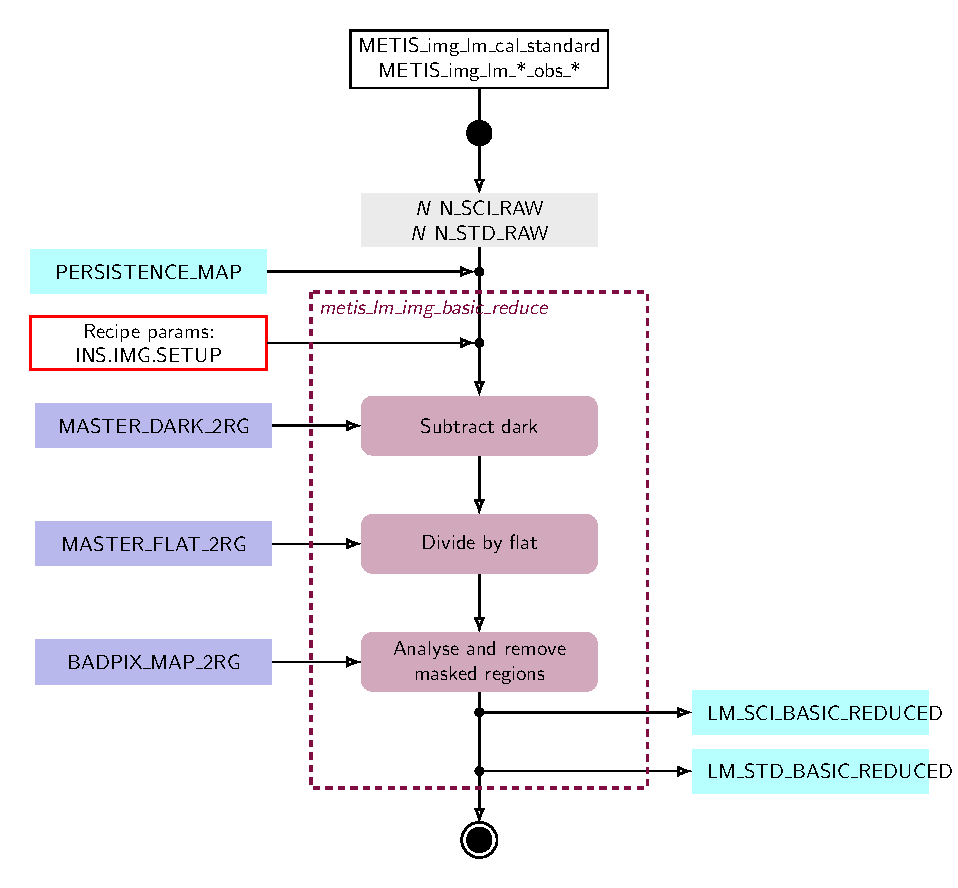
\includegraphics[width=0.6\textwidth]{metis_lm_img_basic_reduce}
  % \resizebox{0.6\textwidth}{0.1\textwidth}{\TODO{\fbox{Figure to be done}}}
  \caption[Recipe: \REC{metis_lm_img_basic_reduce}]{\REC{metis_lm_img_basic_reduce} --
    basic reduction of \CODE{IMG_LM} data.}
  \label{fig:metis_lm_img_basic_reduce}
\end{figure}


\clearpage
\subsubsection{LM-band imaging background subtraction}
\label{lm_img_background}
\label{rec:lm_img_background}
\label{sssec:lm_img_background}
\label{metis_lm_img_background}
\label{rec:metis_lm_img_background}
\label{sssec:metis_lm_img_background}

This recipe estimates and subtracts the background from LM-band
imaging data. Thermal background emission from the atmosphere,
telescope and warm parts of the instrument dominate the photon count
in mid-infrared observations. Accurate determination and removal of
background counts is therefore crucial to make MIR data scientifically
usable.

A set of observations will consist of a number of dithered exposures
of the field, where the offsets are achieved using the internal
chopper of METIS or the with the telescope. For extended objects, the
telescope will be used to perform ``out-of-field dithering'', i.e.\
observe nearby blank patches of sky interlaced with the target
observations. Imaging observations are performed in pupil-tracking
mode, hence angular dithering of the field is automatic.

For in-field-dithered exposures, all dithered exposures will be
averaged to obtain the background estimate. In order to only average
the background contribution, an iterative procedure of object
detection and masking will be employed. Averaging will be done using a
robust estimator of the mean (e.g.\ median).

For extended objects, all out-of-field exposures will be averaged
(with object rejection) and subtracted off the in-field exposures.

This fulfills \REQ{METIS-6085} and \REQ{METIS-6086}.

\TODO{Object catalogues of the target exposures could be created within this
recipe or in a separate recipe. The catalogue should contain for each
object: pixel coordinates ($x$, $y$), world coordinates ($\alpha$,
$\delta$) based on telescope pointing and derotator information, total
counts within an aperture.}

\TODO{Is this good enough for HCI images or do we need more?}

\begin{recipedef}
  Name:             & \REC{metis_lm_img_background}                             \\
  Purpose:          & estimate and subtract background                          \\
  Type:             & Calibration                                               \\
  Templates:        & \TPL{METIS_img_lm_cal_standard}                           \\
                    & \TPL{METIS_img_lm_*_obs_*}                                \\
  Input data:       & \hyperref[dataitem:lm_sci_basic_reduced]{\PROD{LM_SCI_BASIC_REDUCED}}                               \\
                    & \hyperref[dataitem:lm_std_basic_reduced]{\PROD{LM_STD_BASIC_REDUCED}}                               \\
  Matched keywords: & dither position (\CODE{SKY}? \TBD)                        \\
  Algorithm:        & Average all or \CODE{SKY} exposures with object rejection \\
                    & Subtract background                                       \\
  Output data:      & \hyperref[dataitem:lm_sci_bkg]{\PROD{LM_SCI_BKG}}                                         \\
                    & \hyperref[dataitem:lm_std_bkg]{\PROD{LM_STD_BKG}}                                         \\
                    & \hyperref[dataitem:lm_sci_bkg_subtracted]{\PROD{LM_SCI_BKG_SUBTRACTED}}                              \\
                    & \hyperref[dataitem:lm_std_bkg_subtracted]{\PROD{LM_STD_BKG_SUBTRACTED}}                              \\
                    & \hyperref[dataitem:lm_sci_object_cat]{\PROD{LM_SCI_OBJECT_CAT}}                                  \\
                    & \hyperref[dataitem:lm_std_object_cat]{\PROD{LM_STD_OBJECT_CAT}}                                  \\
  QC1 parameters:   & \QC{QC LM IMG BKG MEDIAN}                                 \\
                    & \QC{QC LM IMG BKG MEDIAN DEVIATION}                       \\
  hdrl functions:   & \CODE{hdrl_imagelist_sub_image}                           \\
                    & \CODE{hdrl_imagelist_div_image}                           \\
                    & \CODE{hdrl_catalogue_compute}                             \\
\end{recipedef}

\begin{figure}[hb]
  \centering
  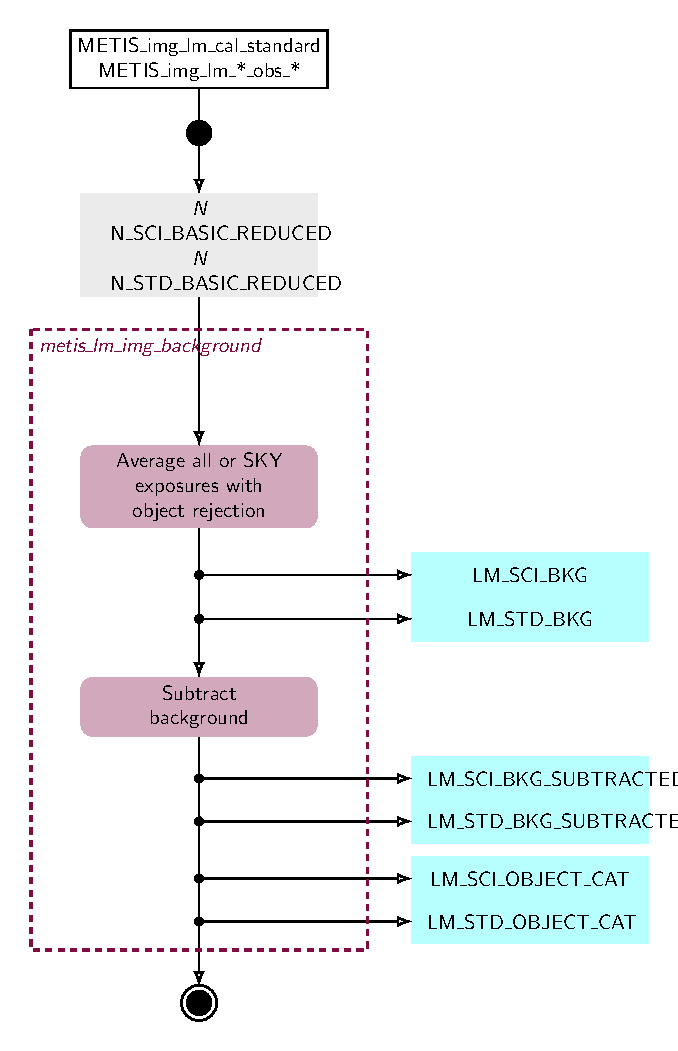
\includegraphics[width=0.6\textwidth]{metis_lm_img_background}
  % \resizebox{0.6\textwidth}{0.1\textwidth}{\TODO{\fbox{Figure to be done}}}
  \caption[Recipe: \REC{metis_lm_img_background}]{\REC{metis_lm_img_background} --
    background estimation and subtraction of dithered \CODE{IMG_LM} data.}
  \label{fig:metis_lm_img_background}
\end{figure}


\clearpage

% \subsubsection{LM-band imaging astrometry calibration}
%
% HB: I've commented the lm_img_astrometry_calib recipe out as it seems
%     not necessary. The two outputs as defined are:
%     - LM_STD_AST_CALIB: this is raw data produced by the
%       template METIS_img_lm_cal_standard, and thus should not be the
%       output of a recipe.
%     - ASTROMETRY_TAB: this seems equivalent to LM_DISTORTION_TABLE, or
%       at least very similar.
%
% \label{lm_img_astrometry_calib}
% \label{rec:lm_img_astrometry_calib}
% \label{sssec:lm_img_astrometry_calib}
% \label{metis_lm_img_astrometry_process}
% \label{rec:metis_lm_img_astrometry_process}
% \label{sssec:metis_lm_img_astrometry_process}
% This recipe is the conversion of the pixel coordinates (X,Y) of objects in an image
% into their corresponding celestial coordinates of right ascension (RA) and
% declination (Dec). The recipe for astrometry calibration involves several
% steps that must be carried out precisely to achieve accurate results.
%
% The first step of the recipe involves identifying a set of reference stars
% in the image, whose coordinates are well known and can be obtained from a
% catalog. This requires careful selection and verification of the reference stars,
% as their accuracy determines the accuracy of the final calibration.
%
% The next step is to use these reference stars to establish a mapping between
% the image's pixel coordinates and their corresponding celestial coordinates. This
% is achieved through a process called plate solving, which involves solving a set
% of mathematical equations to determine the transformation between pixel and celestial
% coordinates. This process requires careful selection of the appropriate transform function
% and calibration parameters.
%
% \begin{recipedef}
%   Name:                & \REC{metis_lm_img_astrometry_process}                                               \\
%   Purpose:             & Determine conversion factor between pixel and world coordinates              \\
%   Type:                & Calibration                                                                  \\
%   Templates:           & \TPL{METIS_img_lm_cal_standard}                                              \\
%   Input data:          & \hyperref[dataitem:lm_std_bkg_subtracted]{\PROD{LM_STD_BKG_SUBTRACTED}}                                                 \\
%                        & photometric standard catalogue                                               \\
%   Matched keywords:    & OBJECT ID                                                                    \\
%                        & FILTER ID                                                                    \\
%   Parameters:          & Distortion correction functions                                              \\
%   Algorithm:           & Measure position of stars in pixel coordinates                               \\
%                        & Compute conversion factor to world coordinates                               \\
%                        & Measure and evaluate the error.                                              \\
%   Output data:         & \hyperref[dataitem:lm_std_ast_calib]{\PROD{LM_STD_AST_CALIB}}                                                      \\
%                        & \hyperref[dataitem:astrometry_tab]{\PROD{ASTROMETRY_TAB}}                                                        \\
%   Expected accuracies: &  $>$0.1$\arcsec$                                                                    \\
%   QC1 parameters:      & \QC{QC LM AST X POS ERR}                                                     \\
%                        & \QC{QC LM AST Y POS ERR}                                                     \\
%                        & \QC{QC LM AST RA POS ERR}                                                    \\
%                        & \QC{QC LM AST DEC POS ERR}                                                    \\
%   hdrl function:       & \CODE{hdrl_strehl_compute}                                                   \\
%                        & \CODE{hdrl_catalogue_compute}                                                \\
%                        & \CODE{hdrl_efficiency_compute}                                               \\
%                        & \CODE{hdrl_imagelist_collapse}                                               \\
% \end{recipedef}
%
% \begin{figure}[hb]
%   \centering
%    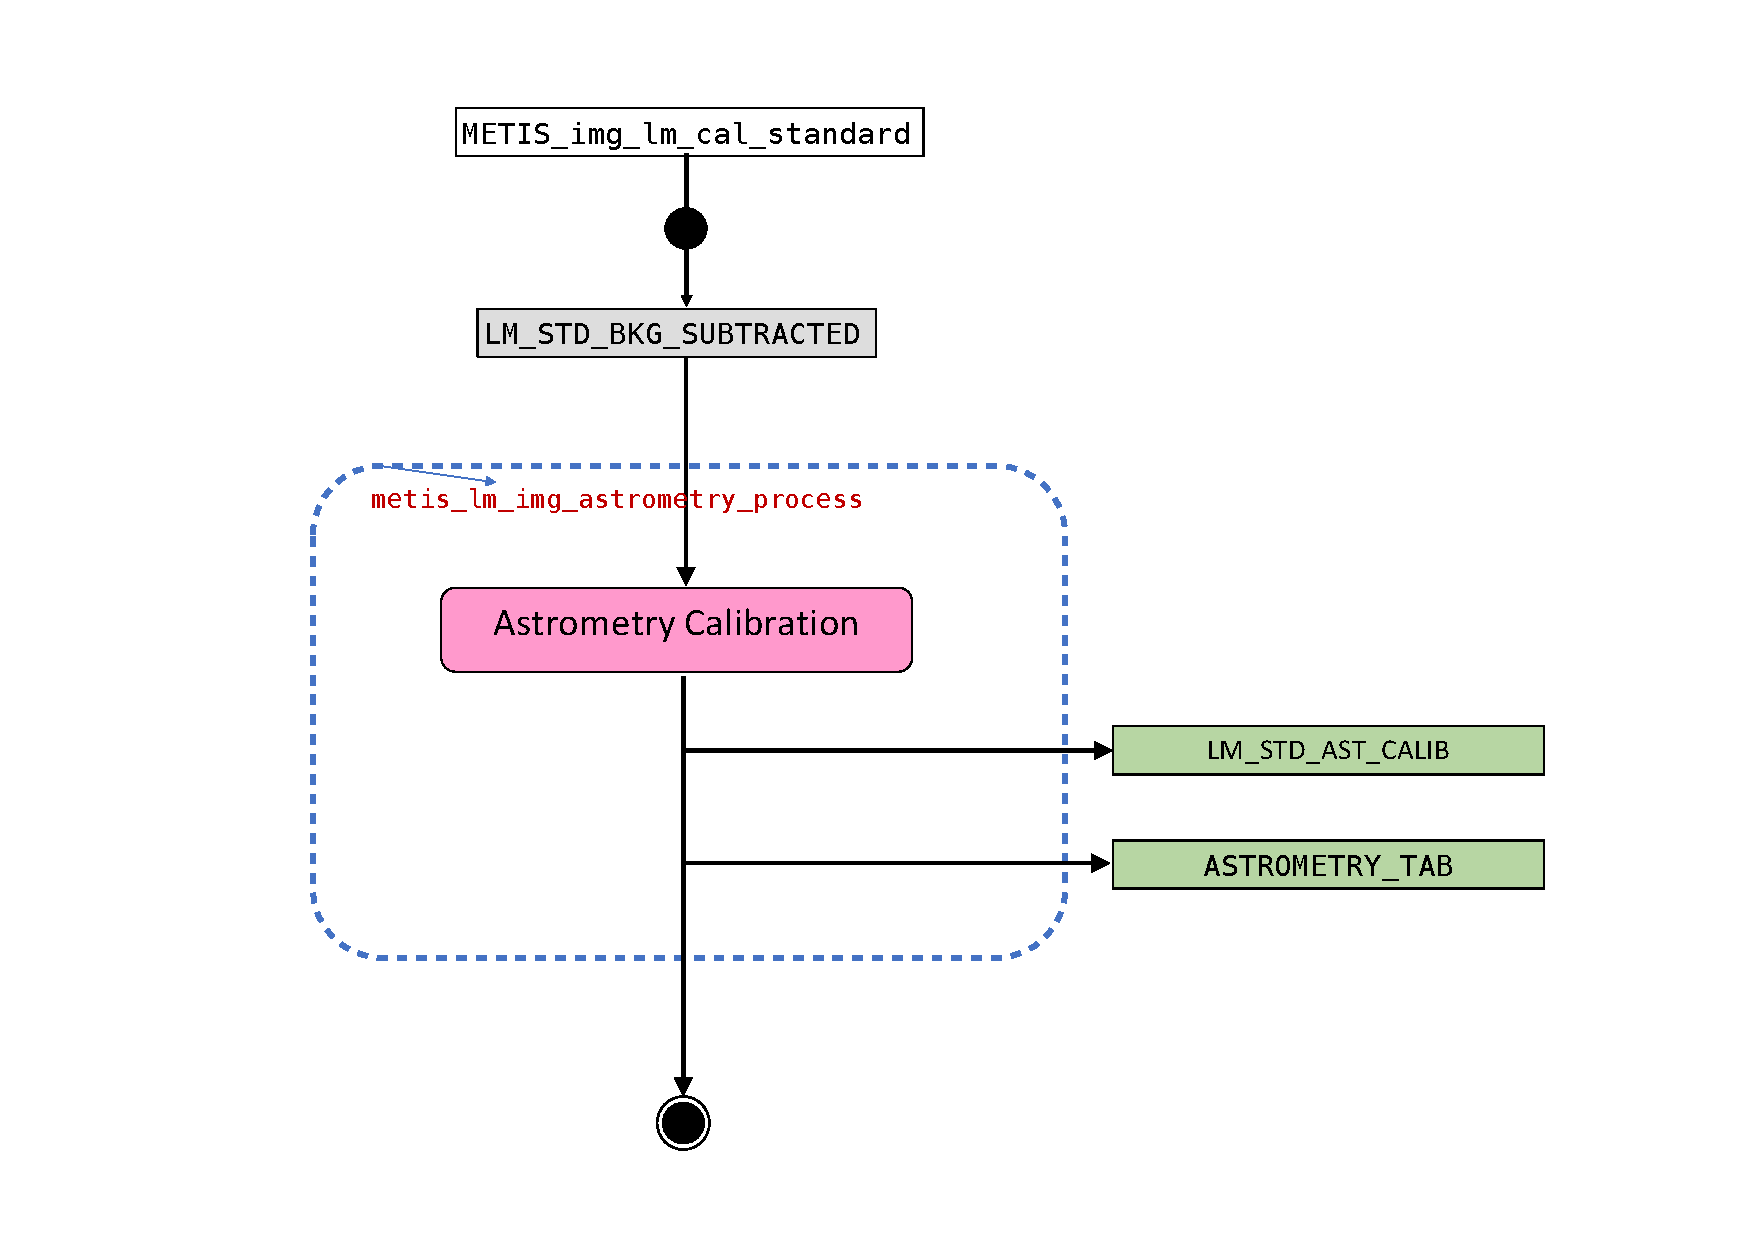
\includegraphics[width=1.0\textwidth]{metis_lm_img_astrometry_process}
%   %\resizebox{0.6\textwidth}{0.1\textwidth}{\TODO{\fbox{Figure to be done}}}
%   \caption[Recipe: \REC{metis_lm_img_astrometry_process}]{\REC{metis_lm_img_astrometry_process} --
%     compute conversion between pixel and sky coordinate}
%   \label{fig:metis_lm_img_astrometry_process}
% \end{figure}
%
%
% \clearpage

\subsubsection{LM-band imaging photometric standard analysis}
\label{lm_img_photstd}
\label{rec:lm_img_photstd}
\label{sssec:lm_img_photstd}

This recipe determines the conversion from ADU to physical units from
a set of reduced exposures of a photometric standard star. The flux of
the star is measured in each exposure in ADU, normalised to an
exposure time of 1~second and averaged over all exposures. In
addition, the exposures are stacked (after recentering on the standard
star, but without derotation) and the flux is measured in the combined
image. Comparison to the tabulated brightness of the star in the
observing filter yields the conversion factor from
$\mathrm{ADU\,s^{-1}}$ to $\mathrm{photons\,\,s^{-1}\,cm^{-2}}$.

QC parameter will include estimates of the sensitivity for the
detection of point sources and surface brightness sensitivity
following \cite{visir_manual}.

\begin{recipedef}\label{rec:metis_lm_img_std_process}
  Name:                & \REC{metis_lm_img_std_process}                                               \\
  Purpose:             & Determine conversion factor between detector counts and physical source flux \\
  Type:                & Calibration                                                                  \\
  Templates:           & \TPL{METIS_img_lm_cal_standard}                                              \\
  Input data:          & \hyperref[dataitem:lm_std_bkg_subtracted]{\PROD{LM_STD_BKG_SUBTRACTED}}                                                 \\
                       & photometric standard catalogue                                               \\
  Matched keywords:    & OBJECT ID                                                                    \\
                       & FILTER ID                                                                    \\
  Parameters:          & None (TBD)                                                                   \\
  Algorithm:           & Call \DRL{calculate_std_flux} to measure flux in input images                      \\
                       & call \DRL{recentre_img} to recentre and stack images                         \\
                       & call \DRL{calculate_std_flux} on the stacked image to get flux of the star in detector units\\
                       & call \DRL{caluculate_std_fluxcal} to calculate the conversion factor to physical units    \\
                       & call \DRL{calculate_detection_limits} to compute measure background noise (std,rms) and compute detection limits \\
  Output data:         & \hyperref[dataitem:lm_std_combined]{\PROD{LM_STD_COMBINED}}                                                       \\
                       & \hyperref[dataitem:fluxcal_tab]{\PROD{FLUXCAL_TAB}}                                                           \\
  Expected accuracies: & \TBD                                                                         \\
  QC1 parameters:      & \QC{QC LM IMG STD BACKGD RMS}                                                \\
                       & \QC{QC LM STD PEAK CNTS}                                                     \\
                       & \QC{QC LM STD APERTURE CNTS}                                                 \\
                       & \QC{QC LM STD STREHL}                                                        \\
                       & \QC{QC LM STD FLUXCONV}                                                      \\
                       & \QC{QC LM STD AIRMASS}                                                       \\
                       & \QC{QC LM SENSITIVITY}                                                       \\
                       & \QC{QC LM AREA SENSITIVIY}                                                   \\
  hdrl functions:      & \CODE{hdrl_strehl_compute}                                                   \\
                       & \CODE{hdrl_catalogue_compute}                                                \\
                       & \CODE{hdrl_efficiency_compute}                                               \\
                       & \CODE{hdrl_imagelist_collapse}                                               \\
\end{recipedef}

\begin{figure}[hb]
  \centering
   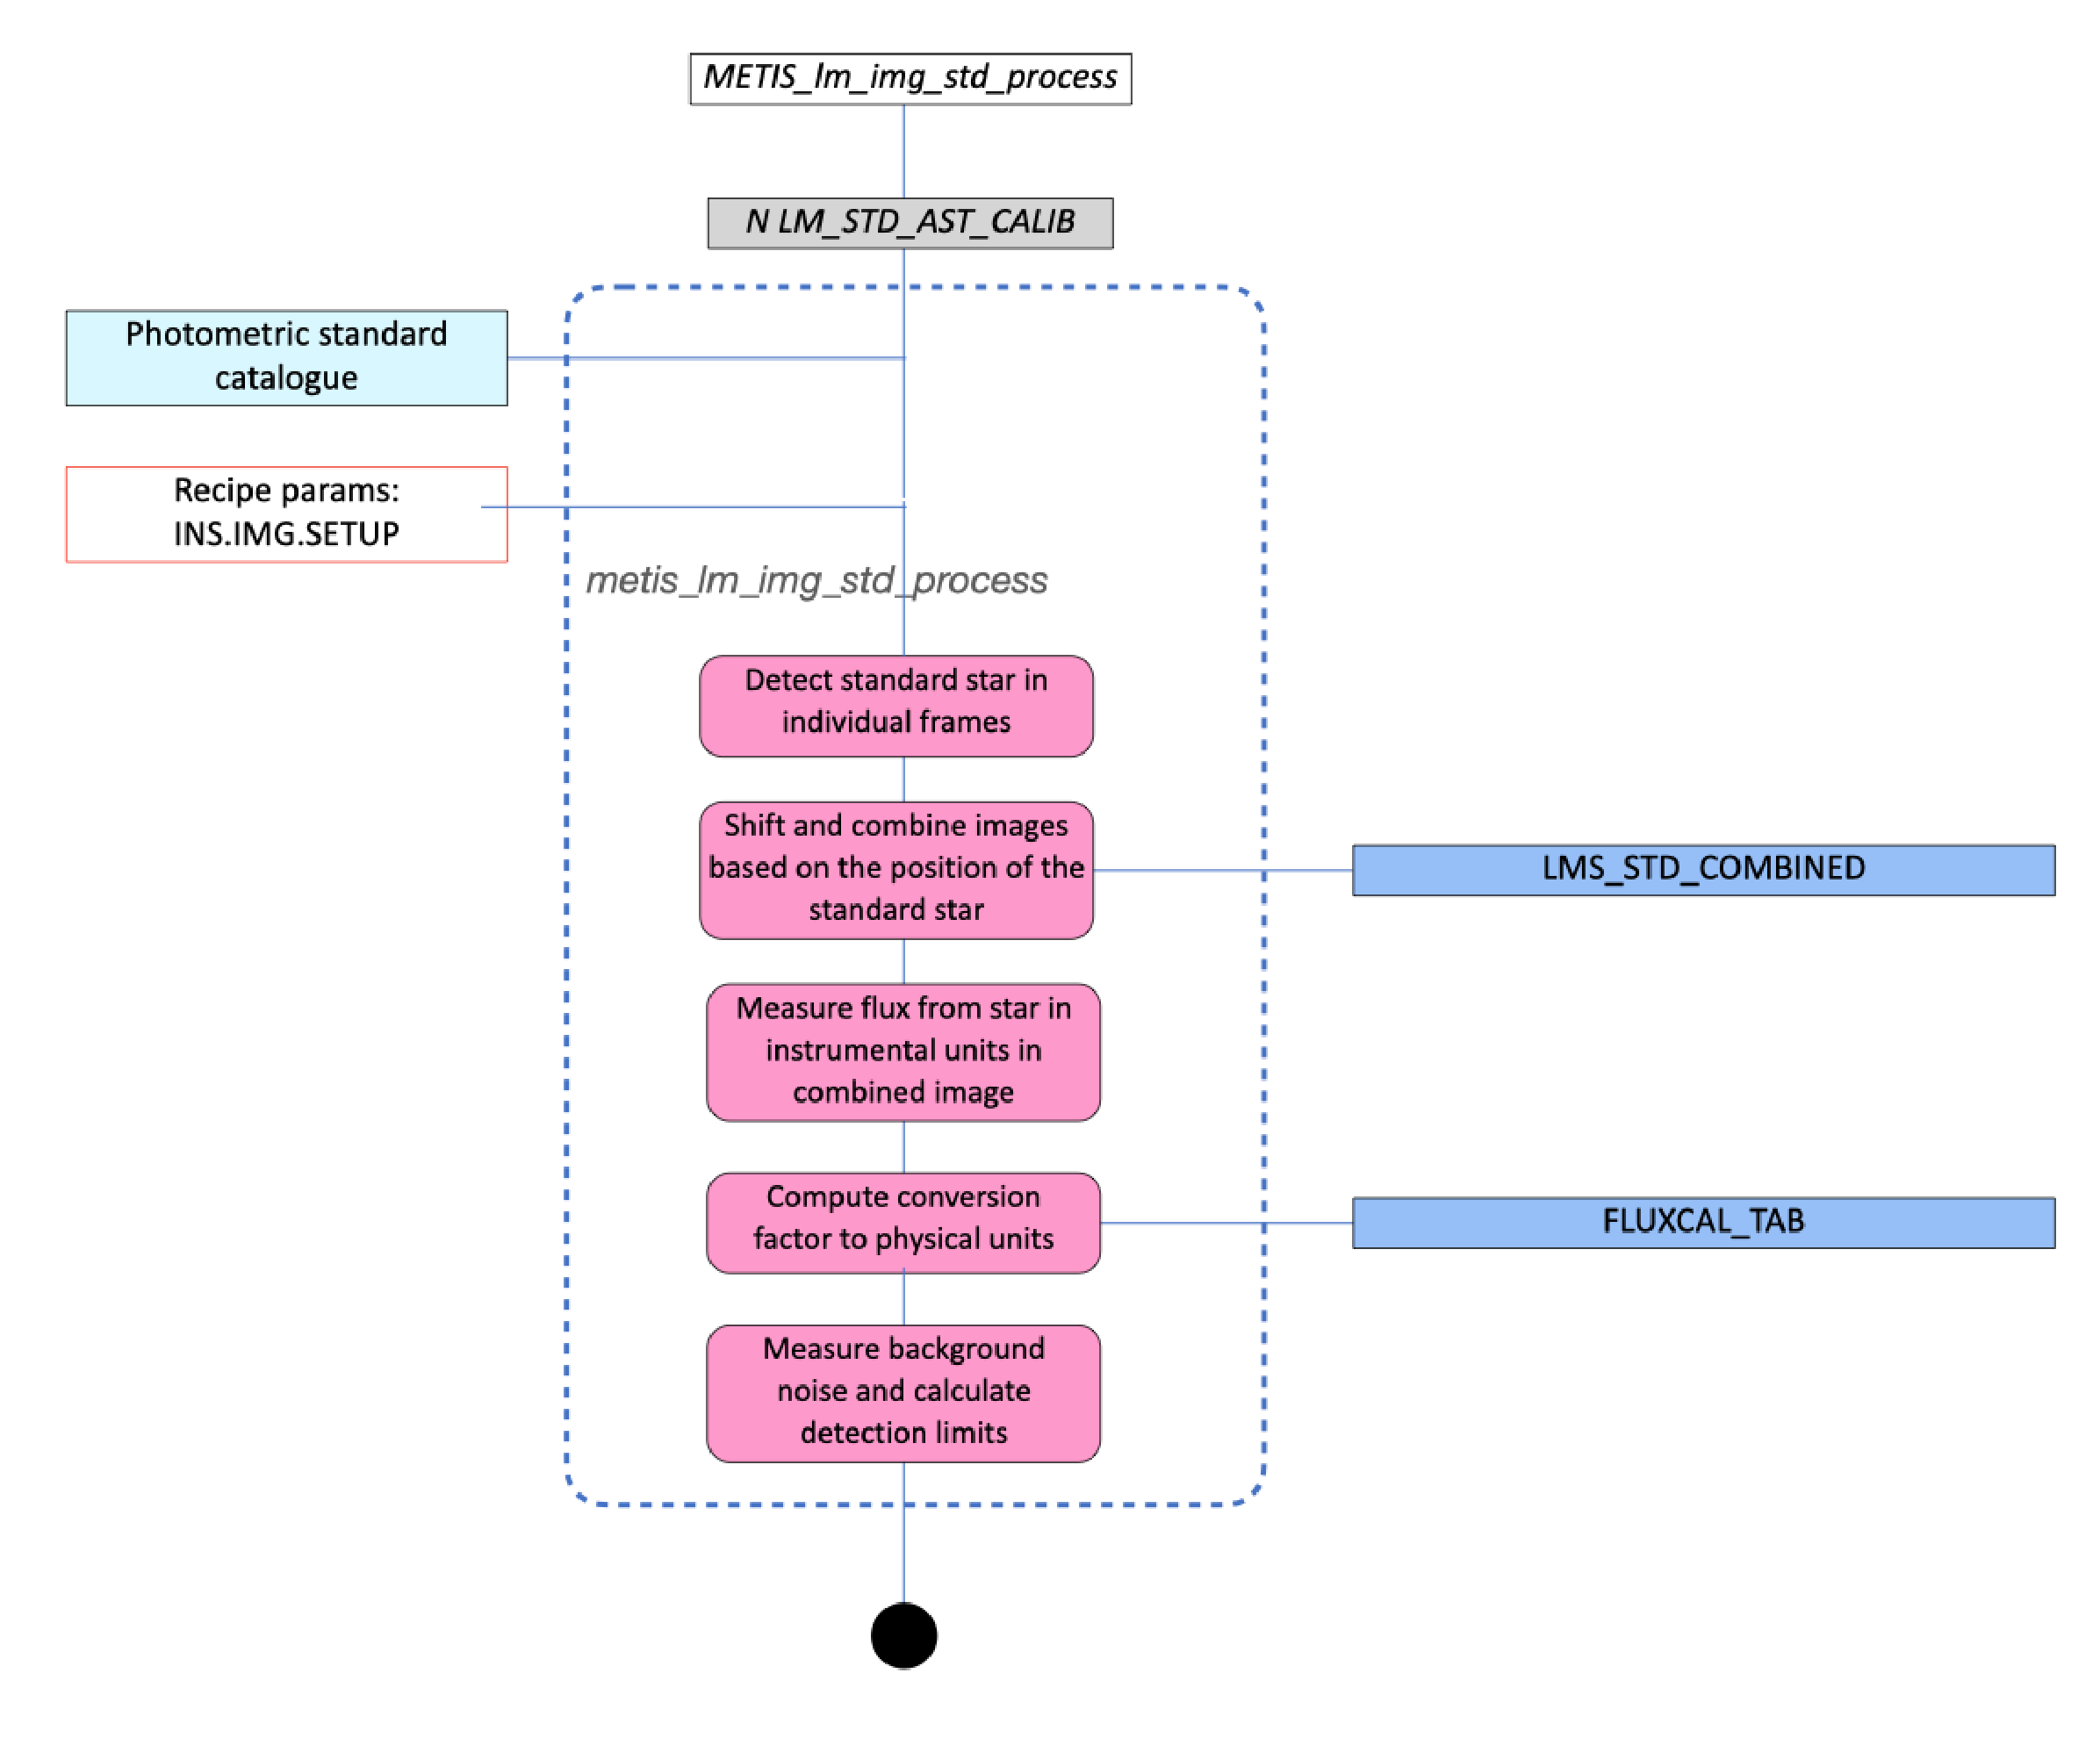
\includegraphics[width=0.6\textwidth]{metis_lm_img_std_process}
  %\resizebox{0.6\textwidth}{0.1\textwidth}{\TODO{\fbox{Figure to be done}}}
  \caption[Recipe: \REC{metis_lm_img_std_process}]{\REC{metis_lm_img_std_process} --
    compute conversion between ADU and physical flux units}
  \label{fig:metis_lm_img_std_process}
\end{figure}

%%%%%%%%%%%%%%%%%%%%%%%%%%%%%%%%%%%%%%%%%%%%%%%%%

\clearpage
\subsubsection{LM-band imaging calibration}
\label{lm_img_calibrate}
\label{rec:lm_img_calibrate}
\label{sssec:lm_img_calibrate}

This recipe applies the flux calibration to the reduced science
images and adds geometric calibration data to the FITS header. The
products of this recipe are fully calibrated individual exposures.

Each image is multiplied by the conversion factor such that pixel
values are in units of photons per second per centimetre squared. The
header of each file receives keyword \FITS{BUNIT} with value %
\CODE{'photon.s**(-1).cm**(-2)'}.

\TODO{Other units may be possible, although additional information is
  needed. For instance,\\ \CODE{photon.s**(-1).cm**(-2).arcsec**(-2)} makes
  values independent of the pixel scale, but requires a distortion map
  (variation of pixel scale across the detector). Energy units (erg
  instead of photons) require knowledge of the spectral energy
  distribution of the sources, in particular for broad-band filters.}

LM-band imaging observations will be performed in pupil-tracking mode
\cite{METIS-operational_concept}, which means that the field rotates
from exposure to exposure.  The information about the field
orientation along with target coordinates, pixel scale and
higher-order polynomial distortion coefficients is written to the FITS
header. The images are not resampled by this recipe, this is left to
\REC{metis_lm_img_sci_postprocess}.



\begin{recipedef}\label{rec:metis_lm_img_calibrate}
  Name:              & \REC{metis_lm_img_calibrate}                     \\
  Purpose:           & Convert science images to physical units         \\
                     & Add distortion information                       \\
  Type:              & Calibration                                      \\
  Templates          & ??                                                 \\
  Input data:        & \hyperref[dataitem:lm_sci_bkg_subtracted]{\PROD{LM_SCI_BKG_SUBTRACTED}}                     \\
                     & \hyperref[dataitem:fluxcal_tab]{\PROD{FLUXCAL_TAB}}                               \\
                     & \hyperref[dataitem:lm_distortion_table]{\PROD{LM_DISTORTION_TABLE}}                       \\
  Matched keywords:  & Filter ID                                        \\
  Parameters:        & None (TBD)                                       \\
  Algorithm:         & call \DRL{lm_scale_image_flux} to Scale image data to ph/s \\
                     & call \DRL{lm_add_header_distortion} to add header information (\FITS{BUNIT}, WCS, etc.) \\
  Output data:       & \hyperref[dataitem:lm_sci_calibrated]{\PROD{LM_SCI_CALIBRATED}}                         \\
  QC1 parameters:    & None                                             \\
  hdrl functions:    & \CODE{hdrl_imagelist_mult_scalar}                \\
\end{recipedef}

\begin{figure}[hb]
  \centering
  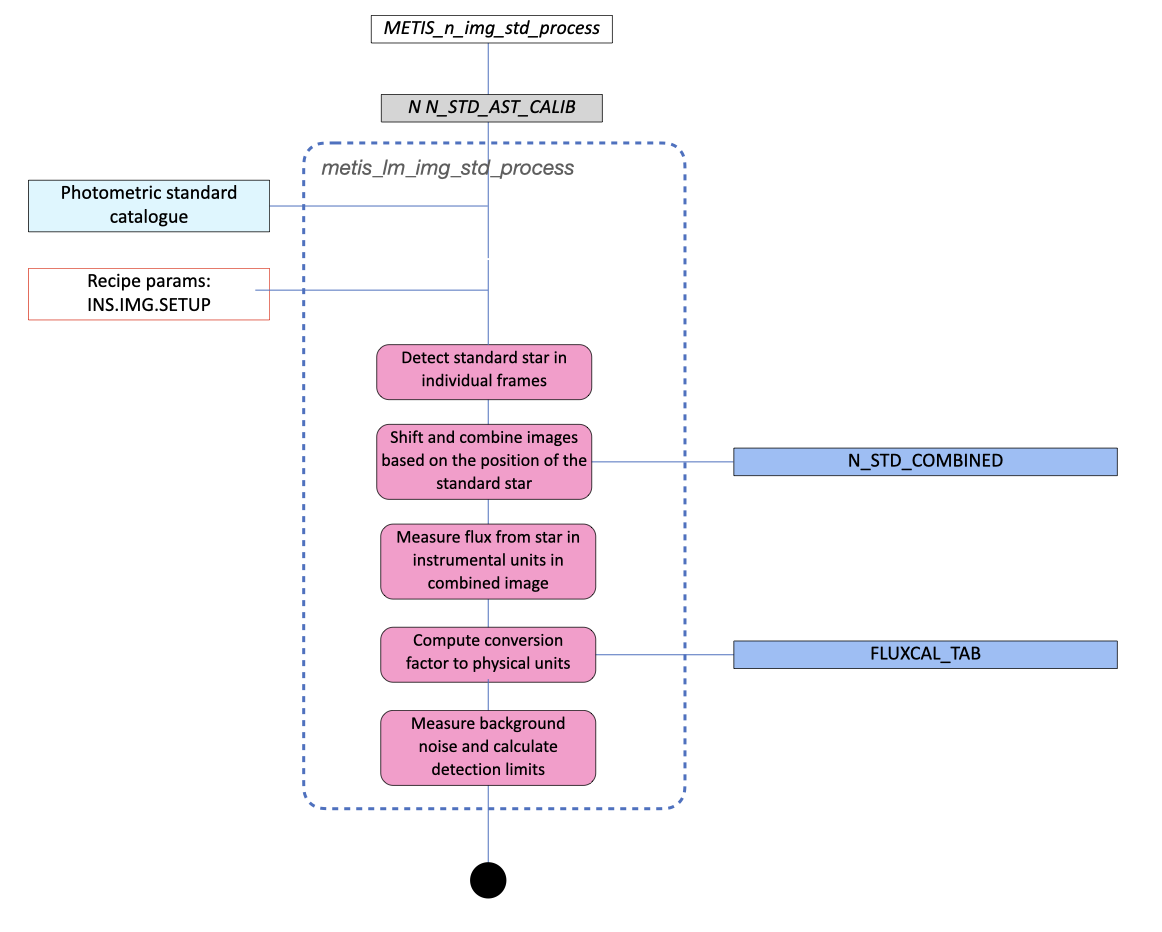
\includegraphics[width=0.6\textwidth]{lm_img_calibrate}
  \caption[Recipe: \REC{metis_lm_img_calibrate}]{\REC{metis_lm_img_calibrate} --
    Convert images to physical flux units and update FITS header}
  \label{fig:metis_lm_img_calibrate}
\end{figure}


%%%%%%%%%%%%%%%%%%%%%%%%%%%%
\clearpage
\subsubsection{LM-band imaging post-processing}
\label{lm_img_postprocess}
\label{rec:lm_img_postprocess}
\label{sssec:lm_img_postprocess}

This recipe coadds a sequence of flux-calibrated,
background-subtracted images (possibly from several observing blocks)
after resampling the images on a common pixel grid defined by a
standard sky projection. The alignment of the images (\FITS{CRVAL}
keywords, rotation) may have to be checked and refined through
cross-correlation of the overlapping images (TBC). The number of input
images contributing to any pixel in the output image (variable due to
dither offsets and bad pixels) will be documented in a contribution
map.

This recipe will only be used in the science-grade pipelines, not at
the observatory. The output fulfills the criteria for \ac{SDP}s and is compliant with \REQ{METIS-6104}.

\begin{recipedef}\label{rec:lm_img_flat}
  Name:                & \REC{metis_lm_img_sci_postprocess}                         \\
  Purpose:             & Coadd reduced images.                                      \\
  Requirements:        & \REQ{METIS-6104}                                           \\
  Templates:           & ---                                                        \\
  Type:                & Science                                                    \\
  Input data:          & Calibrated science images (\PROD{LM_SCI_CALIBRATED})       \\
                       & Associated bad-pixel maps (\PROD{BADPIX_MAP_LM})           \\
  Parameters:          & None (TBD).                                                \\
  Algorithm:           & Check and refine WCS of input images by cross-correlation  \\
                       & \hspace{1em} (on object catalogue or on image).            \\
                       & Determine output pixel grid encompassing all input images. \\
                       & Resample images to output pixel grid.                      \\
                       & Coadd.                                                     \\
  Output data:         & \hyperref[dataitem:lm_sci_coadd]{\PROD{LM_SCI_COADD}} (coadded, mosaiced image)              \\
% TheLM_SCI_COADD_ERROR and LM_SCI_COADD_CONTRIB can be layers in LM_SCI_COADD
%                        & \hyperref[dataitem:lm_sci_coadd_error]{\PROD{LM_SCI_COADD_ERROR}} (coadded, mosaiced error image)  \\
%                        & \hyperref[dataitem:lm_sci_coadd_contrib]{\PROD{LM_SCI_COADD_CONTRIB}} (contribution map)             \\
  Expected accuracies: & TBD                                                        \\
  QC1 parameters:      & \QC{QC LM SCI NEXPOSURE}                                   \\
\end{recipedef}

\begin{figure}[hb]
  \centering
  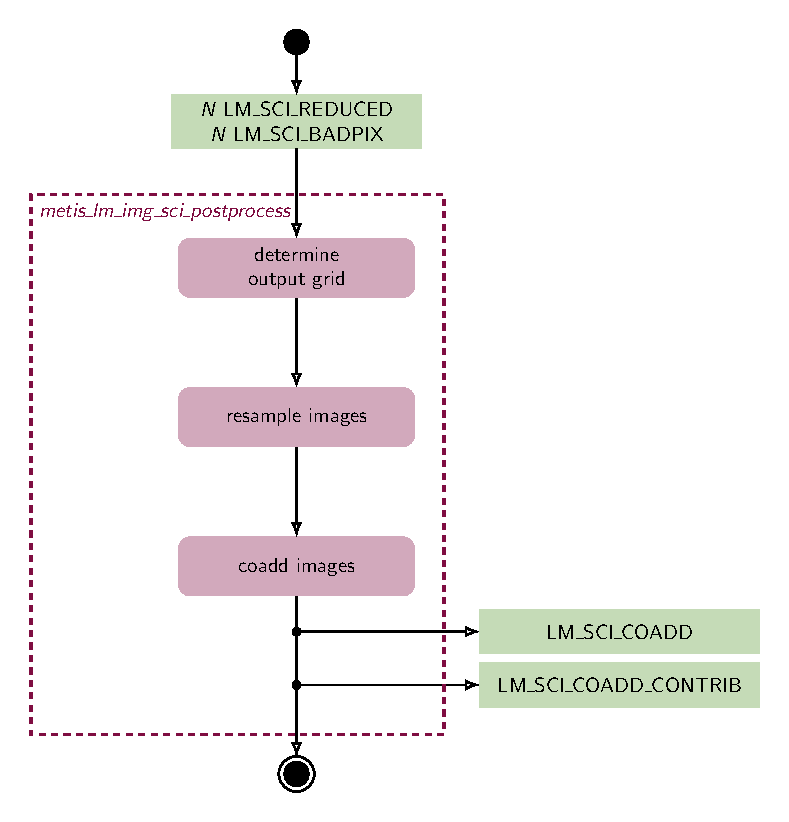
\includegraphics[width=0.7\textwidth]{metis_lm_img_sci_postprocess}
  \caption[Recipe: \REC{metis_lm_img_sci_postprocess}]{%
    \REC{metis_lm_img_sci_postprocess} -- post-processing (coaddition)
    of reduced \CODE{IMG_LM} science frames.}
  \label{fig:metis_lm_img_sci_postprocess}
\end{figure}

%%%%%%%%%%%%%%%%%%%%%%%%%%%%%%%%%%%%%%%%%%%%
\clearpage
\subsubsection{LM-band imaging distortion calibration}
\label{rec:metis_lm_img_distortion}
\label{lm_img_distortion}
\label{rec:lm_img_distortion}
\label{sssec:lm_img_distortion}

Calibration of the imaging distortion is done on an image of a
pin-hole grid mask located in a focal plane within the instrument. The
distortion is described in terms of a polynomial model whose
coefficients can be transformed to WCS keywords and applied to any
other pipeline product. In addition to the distortion table, a map of
pixel scale across the detector will be created.

\begin{recipedef}
  Name:                & \REC{metis_lm_img_distortion}                                   \\
  Purpose:             & Determine optical distortion coefficients for the LM imager.    \\
  Requirements:        & \REQ{METIS-6087}                                                \\
  Templates:           & \TPL{METIS_img_lm_cal_distortion}                               \\
  Type:                & Calibration                                                     \\
  Input data:          & Images of grid mask in WCU-FP2 or CFO-FP2.                      \\
                       & Image with WCU window closed (background)                       \\
                       & Grid of pinhole mask positions \\
                       & Bad pixel map                                                  \\
  Parameters:          & Parameters for fitting routine      \\
                       & \TBD \\
  Algorithm:           & Subtract background image.    (\CODE{hdrl_imagelist_sub_image})                                  \\
                       & Measure location of point source images in frames (\CODE{hdrl_catalogue_create})             \\
                       & call \hyperref[drl:fit_distortion]{\CODE{fit_distortion}} to fit polynomial coefficients to deviations from grid positions.  \\
  Output data:         & \hyperref[dataitem:lm_distortion_table]{\PROD{LM_DISTORTION_TABLE}} \\
                       & \hyperref[dataitem:lm_distortion_map]{\PROD{LM_DISTORTION_MAP}}        \\
                       & \hyperref[dataitem:lm_dist_reduced]{\PROD{LM_DIST_REDUCED}}               \\
  Expected accuracies: & TBD                                                             \\
  QC1 parameters:      & \hyperref[qc:qc_lm_distort_rms]{\QC{QC LM DISTORT RMS}}                                          \\
                       & \hyperref[qc:qc_lm_distort_nsource]{\QC{QC LM DISTORT NSOURCE}}  \\
  hdrl functions:      & \CODE{hdrl_catalogue_create}                                    \\
                       & \CODE{hdrl_imagelist_sub_image}                                \\
\end{recipedef}

\begin{figure}[hb]
  \centering
  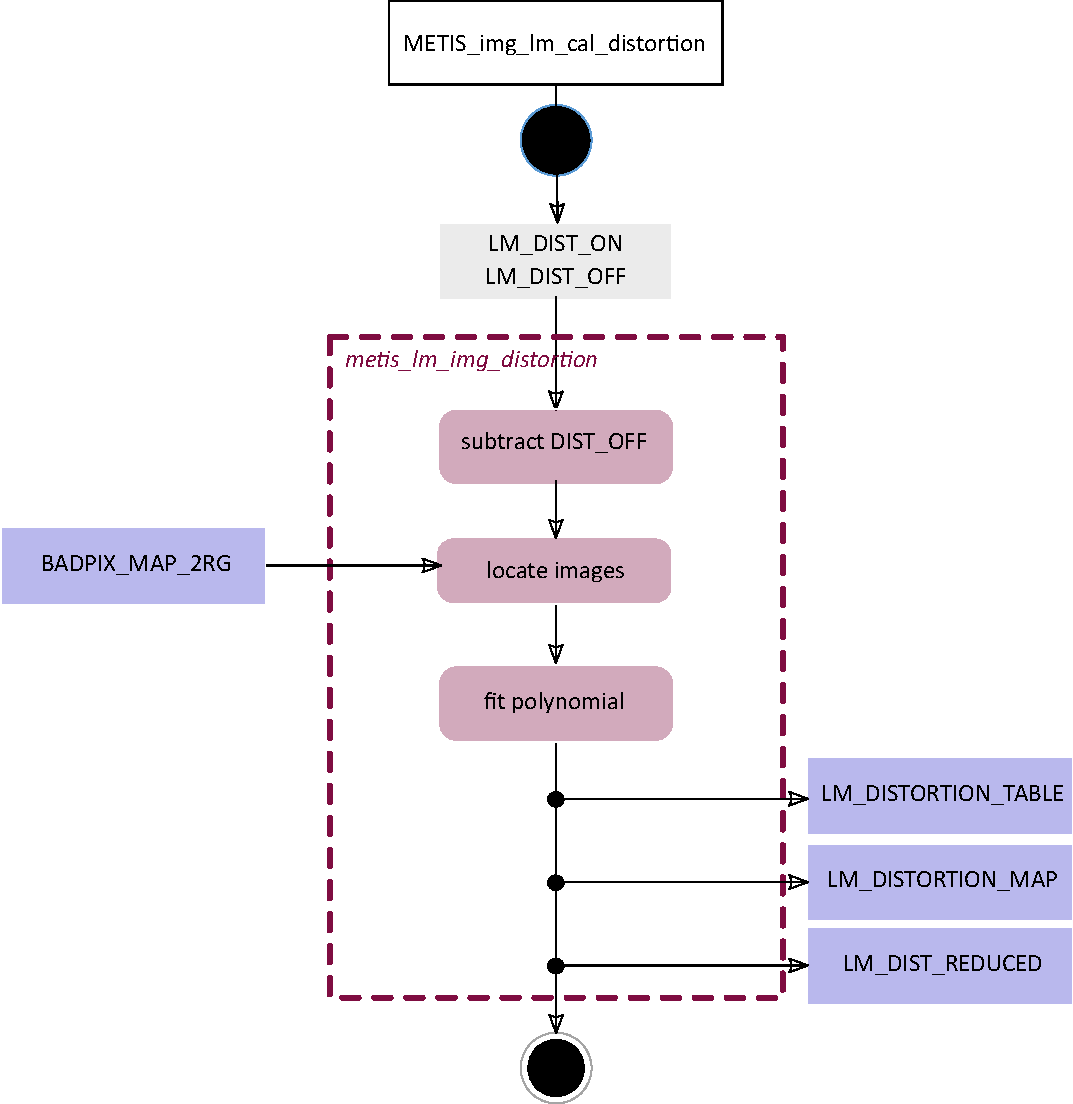
\includegraphics[width=0.6\textwidth]{metis_lm_img_distortion}
  \caption[Recipe: \REC{metis_lm_img_distortion}]{%
    \REC{metis_lm_img_distortion} -- LM IMG distortion calibration}
  \label{fig:metis_lm_img_distortion}
\end{figure}

\FloatBarrier

%%% Local Variables:
%%% TeX-master: "METIS_DRLD"
%%% End:


\subsection{N-band imaging}
\label{ssec:recipes_img_n}

\subsubsection{N-band imaging flatfield}
\label{n_img_flatfield}
\label{rec:n_img_flatfield}
\label{sssec:n_img_flatfield}
\label{n_img_flat}
\label{rec:n_img_flat}
\label{sssec:n_img_flat}
\label{metis_n_img_flat}
\label{rec:metis_n_img_flat}
\label{sssec:metis_n_img_flat}

The purpose of the flat-field calibration is to determine
pixel-to-pixel gain variations and large scale illumination variations
(due to inhomogeneities of optical elements in the telescope or
instrument). Calibration frames are obtained either during day time
using the black-body lamp of the \ac{WCU} (internal flats) or by taken
images of the twilight sky (twilight flats). Advantages and
disadvantages of the two types of flat are discussed in
\cite{METIS-calibration_plan}.

MIR detectors are typically unstable in that they show gain
fluctuations on rather short time scales, hence science exposures may
have a different flat-field structure from those captured by the
calibration flats.  While the GeoSnap detector is expected to be more
stable than the AQUARIUS detector, its stability properties need to be
studied further in order to assess whether science images can be flat
fielded.  N-band flat fields will be taken in any case for quality
control and monitoring purposes.

Since the operational concept for twilight flats needs to be refined
during commissioning at the telescope, the current recipe design is
primarily valid for internal flats.

This recipe creates a master flat for the GeoSnap detector (N-band
imaging) from lamp or sky images matched by various setup parameters
as detailed below.  A set of internal flats includes a number of
exposures with \CODE{LAMP OFF}, which will be used for dark
subtraction. For twilight flats a master dark will be subtracted. The
master flat is obtained by the slope of a linear fit of the pixel
values against the illumination level of the exposures.

The quality control parameters give various statistics for each input
frame (mean, standard deviation, etc.), the standard deviation of the
normalised master flat and the number of bad pixels identified by the
recipe. If a bad-pixel map is provided on input, it is updated,
otherwise a new one is created.

\begin{recipedef}
  Name:                & \REC{metis_n_img_flat}                                         \\
  Purpose:             & Create master flat field for the N-band imaging detector.      \\
  Requirements:        & \REQ{METIS-6098}                                               \\
  Type:                & Calibration                                                    \\
  Templates:           & \TPL{METIS_img_n_cal_InternalFlat}                             \\
                       & \TPL{METIS_img_n_cal_TwilightFlat}                               \\
  Input data:          & Flat field images taken with lamp or sky.                      \\
                       & Master dark (for twilight flats)                               \\
                       & Bad pixel map                                                  \\
  Matched keywords:    & Detector ID                                                    \\
                       & Filter ID                                                      \\
                       & ADC ID                                                         \\
                       & Flat type (internal or twilight)                               \\
                       & possibly others (e.g.\ coronagraphic mask, \TBD)               \\
  Parameters:          & Combination method (\texttt{mean}, \texttt{median},
                         \texttt{sigclip}, \dots)                                       \\
                       & Parameters for combination methods                             \\
                       & Threshold(s) for deviant-pixel identification                  \\
  Algorithm:           & Call \REC{metis_apply_persistance_correction} to apply the
                         persistance correction \\
                       & For internal flats: call \REC{metis_det_dark} with \CODE{LAMP OFF}
                       images to create dark frame. \\
                       & Subtract internal dark or master dark from flat exposures.     \\
                       & call \REC{metis_n_img_flat} to fit slope of pixel values against
                       illumination level. Frames with the same exposure time will be averaged.\\
                       & Compute median or average of input frames to improve statistics.\\
                       & Call \REC{metis_update_lm_flat_mask} to flag deviant pixels. \\
  Output data:         & \PROD{MASTER_IMG_FLAT_N}                                       \\
                       & \PROD{BADPIX_MAP_N}                                            \\
  Expected accuracies: & \TBD                                                           \\
  QC1 parameters:      & \QC{QC N MASTERFLAT RMS}                                       \\
                       & \QC{QC N FLAT NBADPIX}                                         \\
                       & \QC{QC N FLAT MEAN ##}                                         \\
                       & \QC{QC N FLAT RMS ##}                                          \\
  hdrl functions:      & \CODE{hdrl_bpm_fit_compute}                                    \\
                       & \CODE{hdrl_imagelist_collapse}                                 \\
                       & \CODE{hdrl_imagelist_sub_image}                                \\
\end{recipedef}

\begin{figure}[hb]
  \centering
  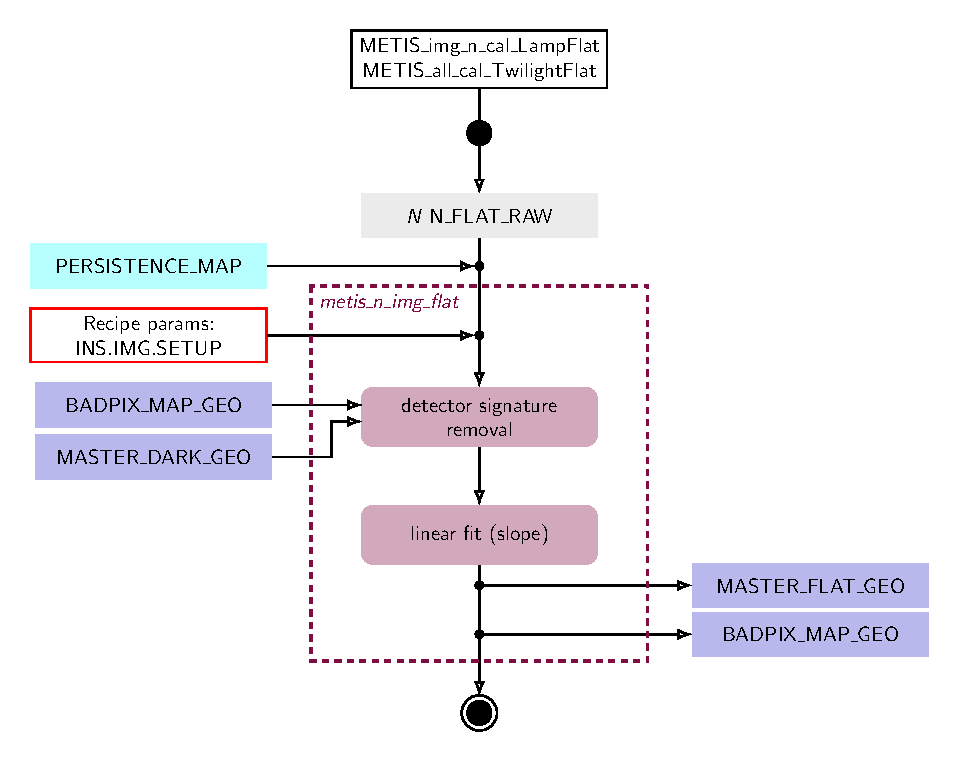
\includegraphics[width=0.6\textwidth]{metis_n_img_flat}
  \caption[Recipe: \REC{metis_n_img_flat}]{\REC{metis_n_img_flat} --
    creation of \CODE{IMG_N} master flatfield}
  \label{fig:metis_n_img_flat}
\end{figure}

%%%%%%%

\subsubsection{N-band imaging chop-nod combination}
\label{img_n_chopnod}
\label{rec:img_n_chopnod}
\label{rec:metis_n_img_chopnod}
\label{sssec:img_n_chopnod}

This recipe combines a set of exposures taken at all positions of a
defined chop-nod pattern and adds/subtracts them into a single
chop/nod difference image. Depending on the actual chop-nod pattern,
this image will contain one or more positive and negative beams.

If flat fielding proves feasible and useful for the GeoSnap detector
the master flat can be applied. If no jitter is applied, i.e.\ if the
beam is at the same detector position for all exposures taken at a
given chop position, then the master flat can be divided into the
final chop-nod difference image. Otherwise, the master flat will have
to be divided into the chop half-cycle images before the jitter
correction is applied.

\begin{recipedef}
  Name:              & \REC{metis_n_img_chopnod}                                    \\
  Purpose:           & chop/nod combination of exposures for background subtraction \\
  Type:              & Calibration, Science                                         \\
 Templates:          & \TPL{METIS_img_n_cal_standard}                              \\
                     & \TPL{METIS_img_n_obs_AutoChopNod}                            \\
                     & \TPL{METIS_img_n_obs_GenericChopNod}                         \\
                     & \TPL{METIS_img_n_cvc_obs_AutoChop}                           \\
%                     & \TPL{METIS_img_n_clc_obs_FixedSkyOffset}                     \\
                     & \TPL{METIS_img_n_cal_psf}                                    \\
  Input data:        & Chopped/nodded science or standard images                    \\
                     & Bad-pixel map                                                \\
  Matched keywords:  & Filter ID                                                    \\
                     & Chop position                                                \\
                     & Nod position                                                 \\
  Parameters:        & TBD                                                          \\
  Algorithm:         & Add/subtract images to subtract background                   \\
  Output data:       & \PROD{N_SCI_BKG_SUBTRACTED}                                  \\
                     & \PROD{N_STD_BKG_SUBTRACTED}                                  \\
  QC1 parameters:    & \QC{N IMG PEAK CNTS}                                         \\
  hdrl functions:    & \CODE{hdrl_imagelist_collapse}                               \\
\end{recipedef}

\begin{figure}[hb]
  \centering
   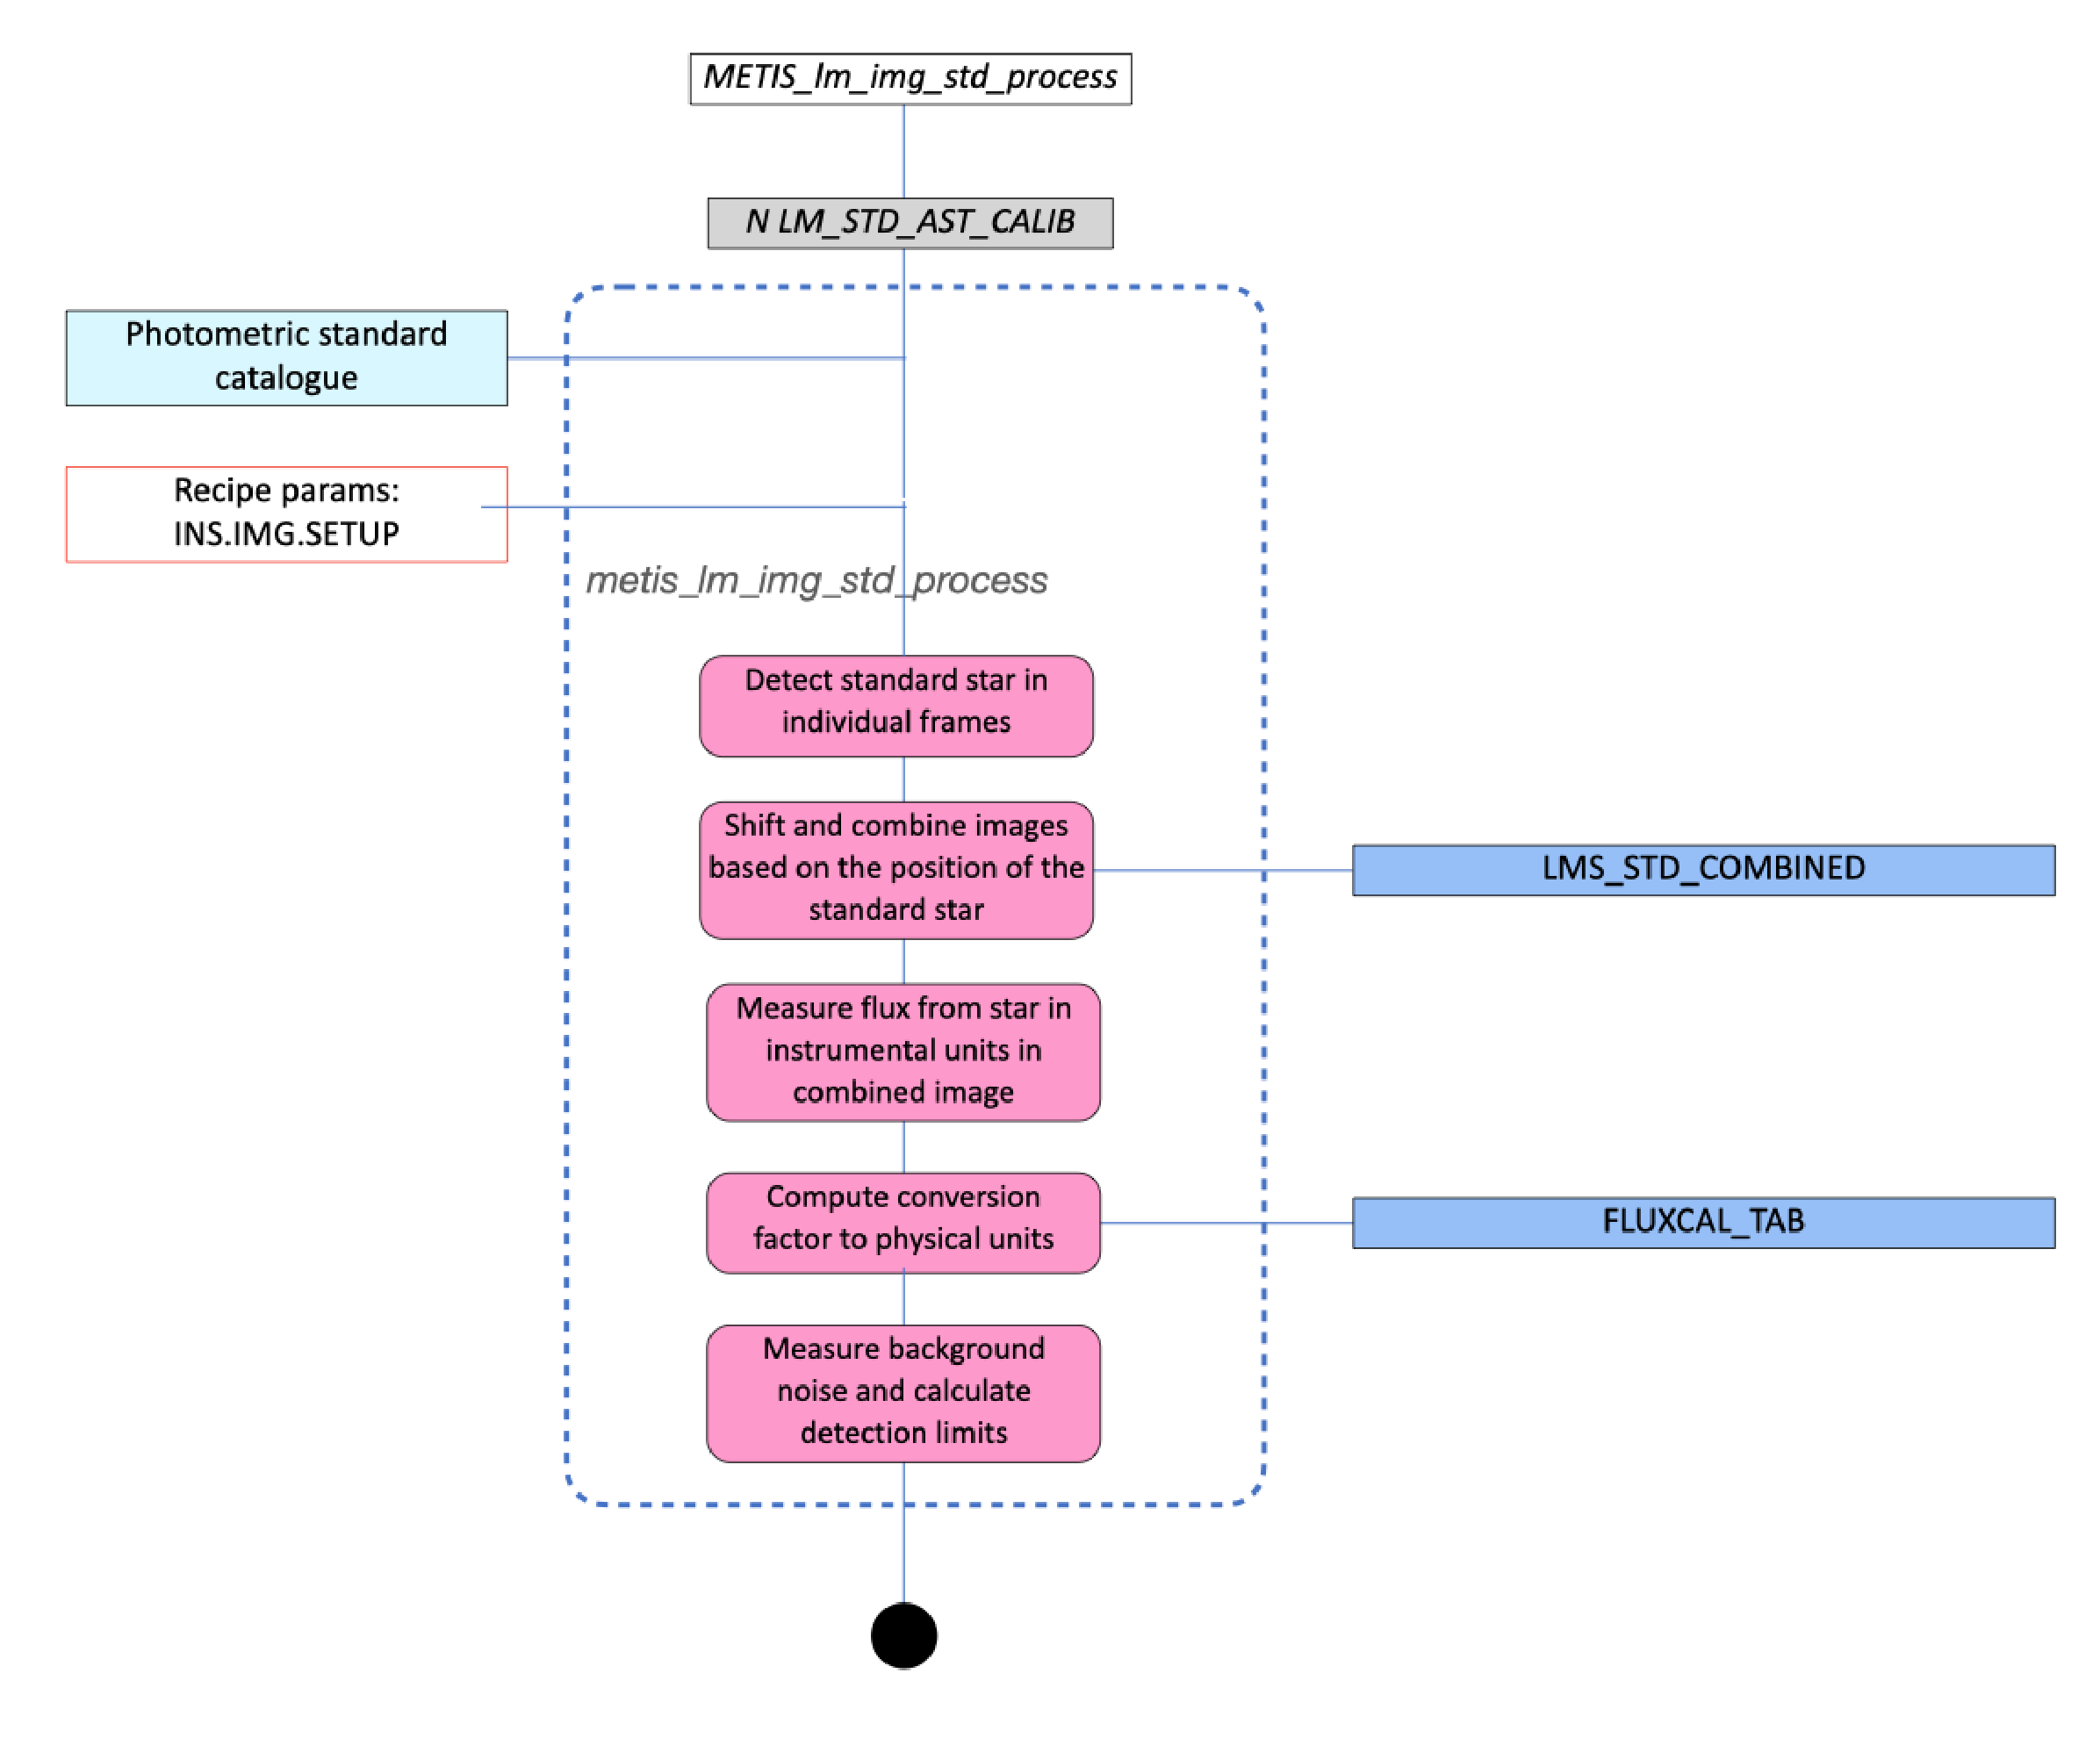
\includegraphics[width=0.6\textwidth]{metis_lm_img_std_process}
  \resizebox{0.6\textwidth}{0.1\textwidth}{\TODO{\fbox{Figure to be done}}}
  \caption[Recipe: \REC{metis_n_img_chopnod}]{\REC{metis_n_img_chopnod} --
    Combination of chop/nodded images.}
  \label{fig:metis_n_img_chopnod}
\end{figure}

%%%%%%%%%%%%%%%%%%%
\clearpage
\subsubsection{N-band imaging photometric standard analysis}
\label{n_img_std_process}
\label{rec:n_img_std_process}
\label{ssec:n_img_std_process}
\label{sssec:n_img_std_process}
\label{metis_n_img_std_process}
\label{rec:metis_n_img_std_process}
\label{sssec:metis_n_img_std_process}

This recipe determines the conversion from ADU to physical units from
a chop-nod difference image of a photometric standard star.  The flux
of the standard star is measured in each of the beams of the chop-nod
difference image, averaged and normalised to an exposure time of
1~second. Comparison to the tabulated brightness of the star in the
observing filter yields the conversion factor from
$\mathrm{ADU}\,\mathrm{s}^{-1}$ to
$\mathrm{photons}\,\mathrm{s}^{-1}\,\mathrm{cm}^{-2}$.

QC parameters will include estimates of the sensitivity for the
detection of point sources and surface brightness sensitivity
following \cite{visir_manual}.

\begin{recipedef}
  Name:                & \REC{metis_n_img_std_process}                                                 \\
  Purpose:             & Determine conversion factor between detector counts and physical source flux. \\
  Type:                & Calibration                                                                   \\
  Templates:           & \TPL{METIS_img_n_cal_standard}                                                \\
  Input data:          & \CODE{N_STD_BKG_SUBTRACTED}                                                   \\
                       & photometric standard catalogue                                                \\
  Matched keywords:    & Object ID                                                                     \\
                       & Filter ID                                                                     \\
  Parameters:          & None (TBD)                                                                    \\
  Algorithm:           & call \CODE{n_calculate_std_flux} to measure the flux in all beams\\
                       & average and normalize flux values \\
                       & call \CODE{calculate_std_fluxcal} to calculate conversion factor to physical units   \\
                       & call \CODE{calculate_detection_limits} to compute measured background noise (std, rms) and compute detection limits \\
  Output data:         & \PROD{FLUXCAL_TAB}                                                            \\
  Expected accuracies: & \TBD                                                                          \\
  QC1 parameters:      & \QC{QC N STD PEAK CNTS}                                                       \\
                       & \QC{QC N STD APERTURE CNTS}                                                   \\
                       & \QC{QC N STD STREHL}                                                          \\
                       & \QC{QC N STD FLUXCONV}                                                        \\
                       & \QC{QC N STD AIRMASS}                                                         \\
                       & \QC{QC N SENSITIVITY}                                                         \\
                       & \QC{QC N AREA SENSITIVITY}                                                    \\
  hdrl functions:      & \CODE{hdrl_catalogue_create}                                                  \\
                       & \CODE{hdrl_strehl_compute}                                                    \\
\end{recipedef}

\begin{figure}[hb]
  \centering
   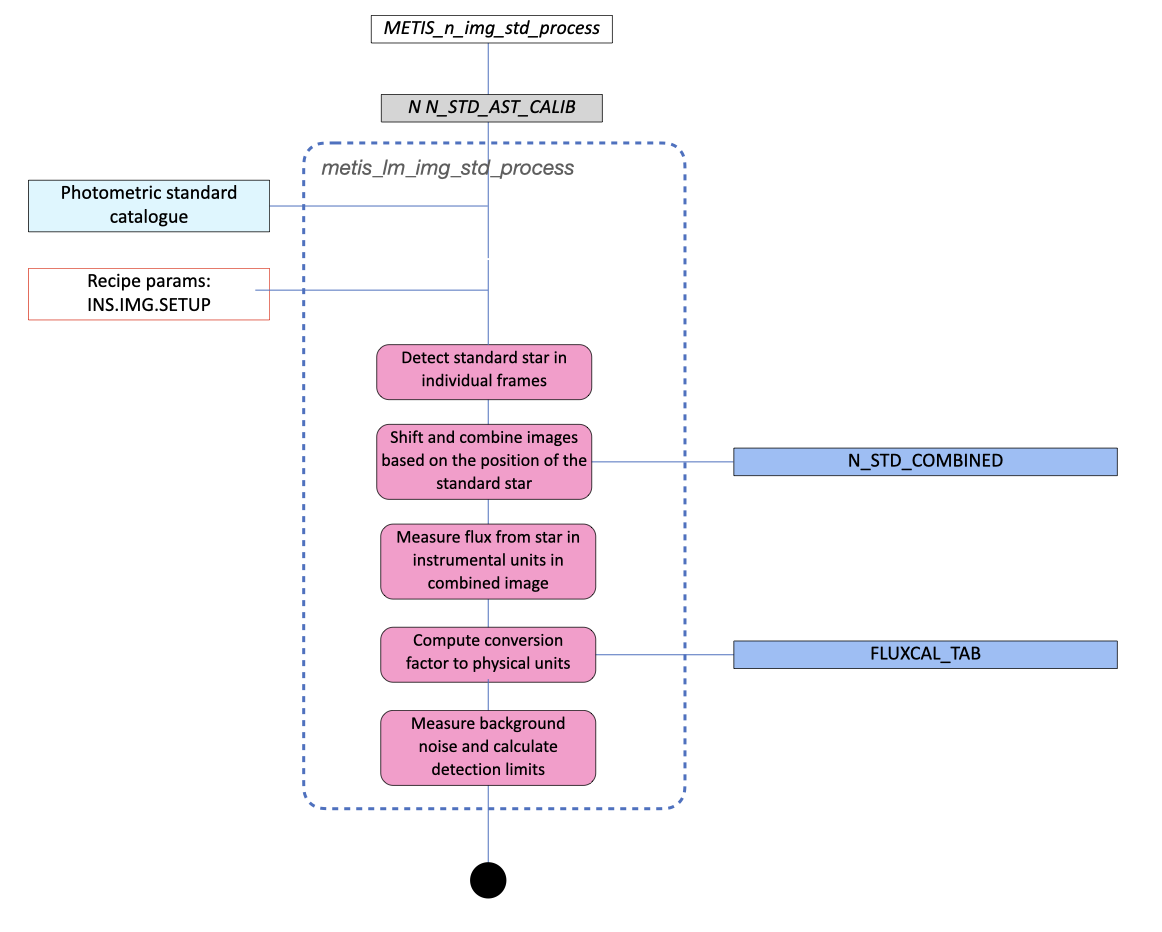
\includegraphics[width=0.6\textwidth]{metis_n_img_std_process}
  %\resizebox{0.6\textwidth}{0.1\textwidth}{\TODO{\fbox{Figure to be done}}}
  \caption[Recipe: \REC{metis_n_img_std_process}]{\REC{metis_n_img_std_process} --
    compute conversion between ADU and physical flux units.}
  \label{fig:metis_n_img_std_process}
\end{figure}


%%%%%%%%%%%%%%%%%%%%%
\clearpage

\subsubsection{N-band imaging calibration}
\label{n_img_calibrate}
\label{rec:n_img_calibrate}
\label{sssec:n_img_calibrate}
\label{rec:metis_n_img_calibrate}

This recipe applies the flux calibration to the chop-nod difference
image. A unique geometric calibration is not possible at this point,
although one could take one of the beams (e.g.\ the positive beam in a
parallel two-point chop-nod pattern) as reference for a
WCS. Distortion information can be added without a reference point as
it pertains to the detector/focal plane, not to the field.

The products of this recipe is the fully calibrated chop-nod
difference image.

The image is multiplied by the conversion factor such that pixel
values are in units of photons per second per centimetre squared. The
header receives the keyword \FITS{BUNIT} with value %
\CODE{'photon.s**(-1).cm**(-2)'}.

\begin{recipedef}
  Name:              & \REC{metis_n_img_calibrate}                      \\
  Purpose:           & Convert science image to physical units          \\
                     & Add distortion information                       \\
  Type:              & Calibration                                      \\
  Templates:         &                                                  \\
  Input data:        & \PROD{N_SCI_BKG_SUBTRACTED}                      \\
                     & \PROD{FLUXCAL_TAB}                               \\
                     & \PROD{N_DISTORTION_TABLE}                        \\
  Matched keywords:  & Filter ID                                        \\
  Parameters:        & TBD                                              \\
  Algorithm:         & call \REC{n_scale_image_flux} to Scale image data to ph/s \\
                     & call \REC{n_add_header_distortion} to add header information (\FITS{BUNIT}, etc.)\\
  Output data:       & \PROD{N_SCI_CALIBRATED}                          \\
  QC1 parameters:    & None                                             \\
\end{recipedef}

\begin{figure}[hb]
  \centering
   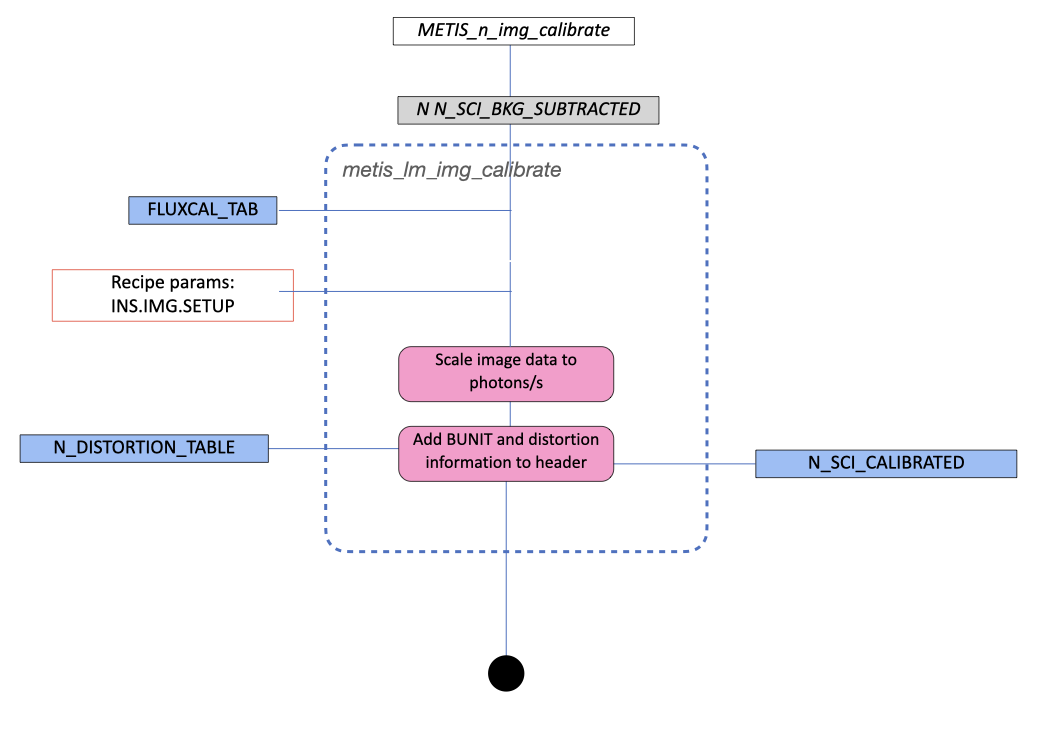
\includegraphics[width=0.6\textwidth]{metis_n_img_calibrate}
  \caption[Recipe: \REC{metis_n_img_calibrate}]{\REC{metis_n_img_calibrate} --
    convert image to physical flux units and update FITS header}
  \label{fig:metis_n_img_calibrate}
\end{figure}

%%%%%%%%%%%%%
\clearpage

\subsubsection{N-band imaging restoration}
\label{n_img_restoration}
\label{rec:n_img_restoration}
\label{sssec:n_img_restoration}

This recipe attempts to combine the positive and negative beams of the
chop-nod difference image into a single positive image of the
source. For compact sources with a size smaller than half the distance
between the beams, it suffices to cut out small regions around the
source images and add the with the appropriate signs to obtain a
single image.

Algorithms for image restoration of extended sources exist but it
remains \TBD\ whether these are sufficiently simple and robust to be
included in the pipeline (cf.\ Sect.~8.8 of \cite{DRLS}).

\begin{recipedef}
  Name:              & \REC{metis_n_img_restore}                                     \\
  Purpose:           & Restore a single positive beam from chop-nod difference image \\
  Type:              & Science                                                       \\
  Input data:        & \CODE{N_SCI_CALIBRATED}                                       \\
  Parameters:        & size of cutout region                                         \\
  Algorithm:         & Cut regions around beams                                      \\
                     & Add regions with appropriate signs                            \\
  Output data:       & \PROD{N_SCI_RESTORED}                                         \\
  QC1 parameters:    & None                                                          \\
  hdrl functions:    & \CODE{hdrl_imagelist_collapse}                                \\
\end{recipedef}

\begin{figure}[hb]
  \centering
  % 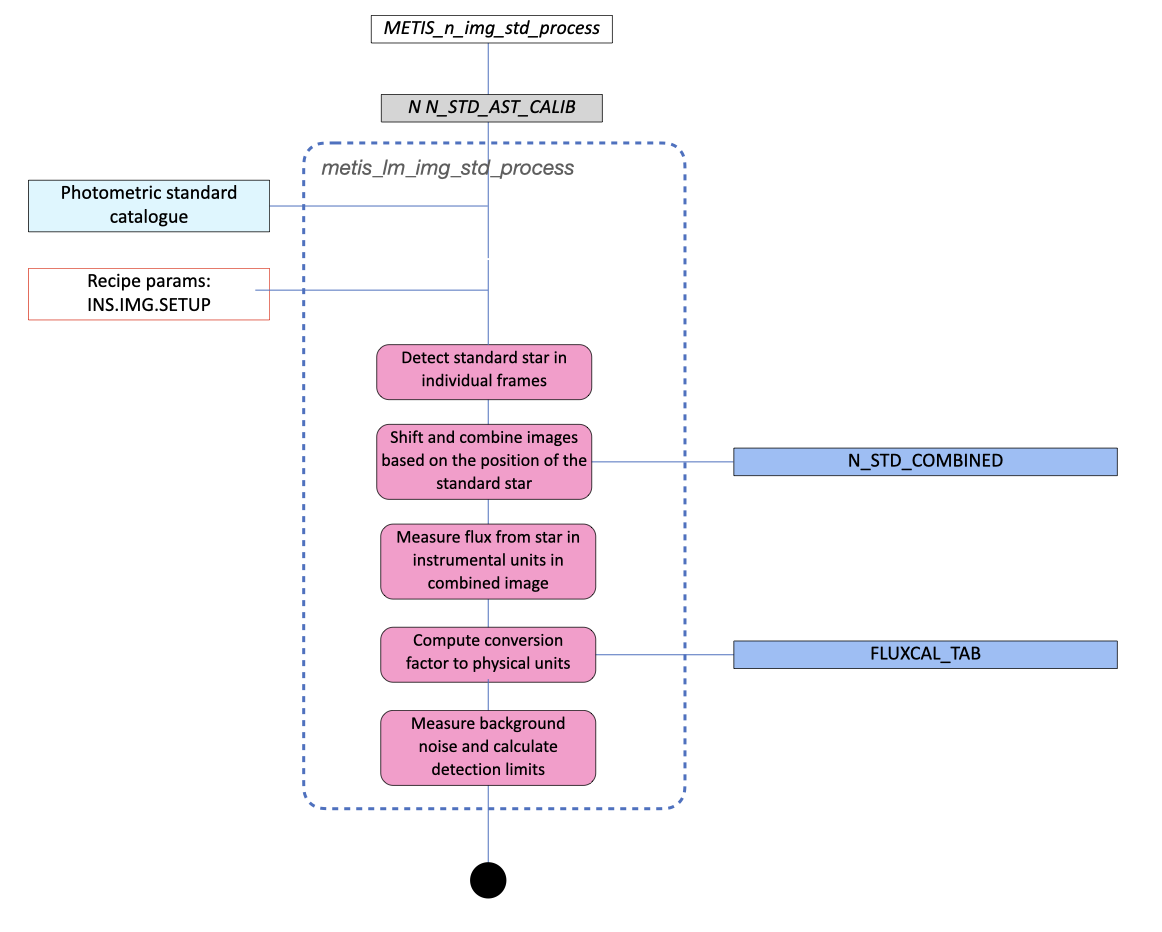
\includegraphics[width=0.6\textwidth]{metis_n_img_std_process}
  \resizebox{0.6\textwidth}{0.1\textwidth}{\TODO{\fbox{Figure to be done}}}
  \caption[Recipe: \REC{metis_n_img_restore}]{\REC{metis_n_img_restore} --
    Create a single positive image from chop-nod difference image}
  \label{fig:metis_n_img_restore}
\end{figure}

%%%%%%%%%%%%%%
\clearpage
\subsubsection{N-band imaging distortion calibration}
\label{n_img_distortion}
\label{rec:n_img_distortion}
\label{sssec:n_img_distortion}

Calibration of the imaging distortion is done on an image of a pin
hole mask located in a focal plane within the instrument. The
distortion is described in terms of a polynomial model whose
coefficients can be transformed to WCS keywords and applied to any
other pipeline product. In addition to the distortion table, a map of
pixel scale across the detector will be created.

\begin{recipedef}
  Name:                & \REC{metis_n_img_distortion}                                   \\
  Purpose:             & Determine optical distortion coefficients for the N imager.    \\
  Templates:           & \TPL{METIS_img_n_cal_distortion}                               \\
  Type:                & Calibration                                                    \\
  Input data:          & Images of grid mask in WCU-FP2 or CFO-FP2.                     \\
                       & Image with WCU window closed (background).                     \\
                       & Grid of pinhole mask positions \\
                       & Bad pixel map                                                  \\
  Parameters:          & Parameters for fitting routine \\
                       & \TBD \\
  Algorithm:           & Subtract background image.  (\CODE{hdrl_imagelist_sub_image})                                       \\
                       & Measure location of point source images in frames.   (\CODE{hdrl_catalogue_create})            \\
                       & call \hyperref[drl:fit_distortion]{\CODE{fit_distortion}} to fit polynomial coefficients to deviations from grid positions. \\
  Output data:         & \hyperref[dataitem:n_distortion_table]{\PROD{N_DISTORTION_TABLE}} \\
                       & \hyperref[dataitem:n_distortion_map]{\PROD{N_DISTORTION_MAP}}        \\
                       & \hyperref[dataitem:n_dist_reduced]{\PROD{N_DIST_REDUCED}}             \\
  Expected accuracies: & TBD                                                            \\
  QC1 parameters:      & \hyperref[qc:qc_n_distort_rms]{\QC{QC N DISTORT RMS} }                                         \\
                       & \hyperref[qc:qc_n_distort_nsource]{\QC{QC LM DISTORT NSOURCE}}  \\
  hdrl functions:      & \CODE{hdrl_catalogue_create}                                   \\
                       & \CODE{hdrl_imagelist_sub_image}                                \\
\end{recipedef}

\begin{figure}[hb]
  \centering
  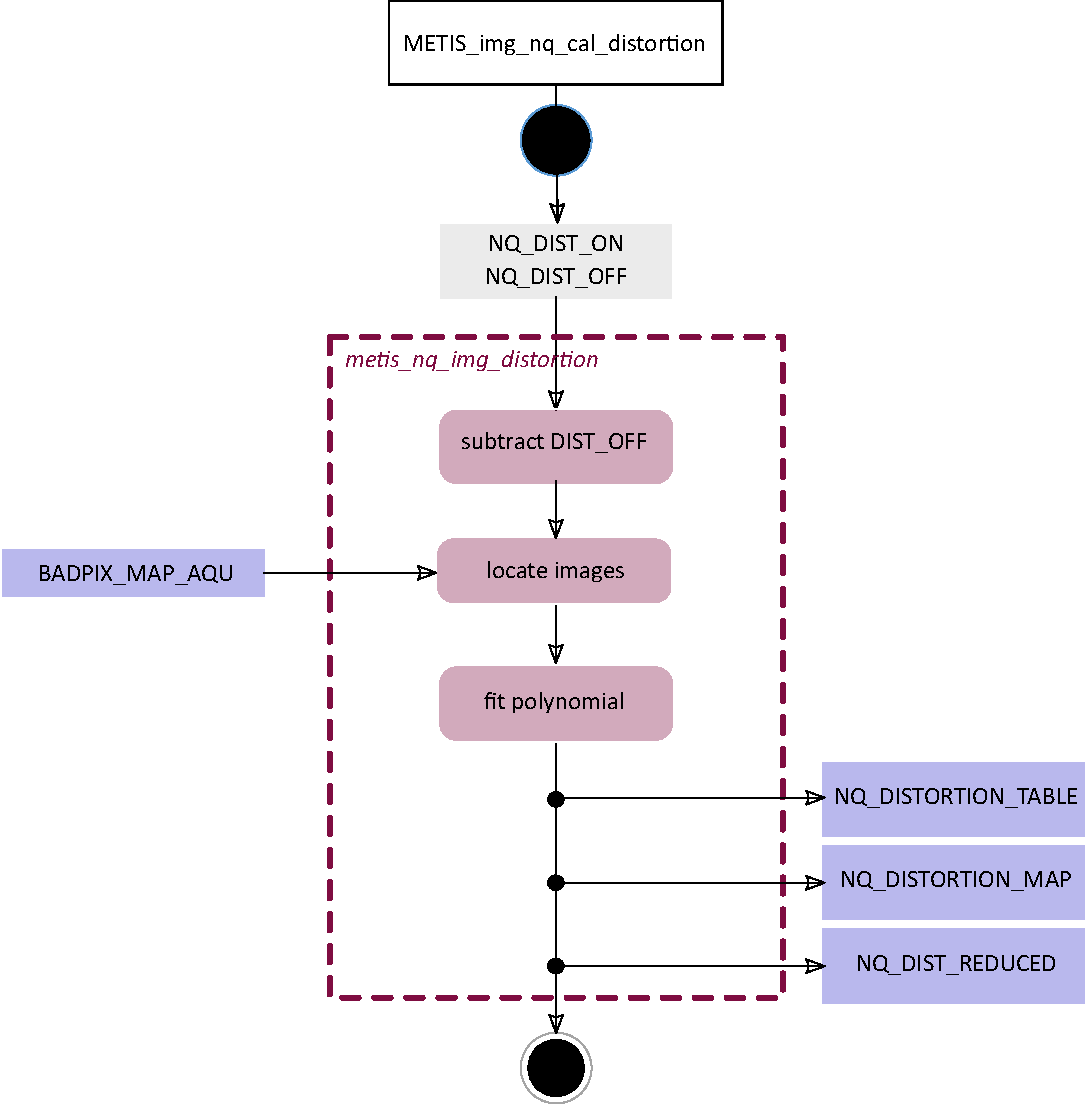
\includegraphics[width=0.6\textwidth]{metis_n_img_distortion}
  \caption[Recipe: \REC{metis_n_img_distortion}]{%
    \REC{metis_n_img_distortion} -- \CODE{IMG_N} distortion calibration}
  \label{fig:metis_n_img_distortion}
\end{figure}

%%% Local Variables:
%%% TeX-master: "METIS_DRLD"
%%% End:

\clearpage
\subsection{Long-slit spectroscopy, LM band}
\label{ssec:recipes_lss_lm}

A draft of the reduction cascade is shown in
Figs.~\ref{Fig:LMLssAssomap1} and \ref{Fig:LMLssAssomap2} together with the data processing table
(Tables~\ref{Tab:LMLssDatProc1} and ~\ref{Tab:LMLssDatProc2}). The first part aims to update the static calibration database, in particular the creation of the gain map (\hyperref[Sec:detector_calibration]{\REC{metis_det_lingain}}) and the determination of the \ac{ADC} slitlosses (\hyperref[rec:metis_lm_adc_slitloss]{\REC{metis_lm_adc_slitloss}}). These are executed only when an update is required, e.g. after a major instrument interention or on yearly basis. The second part comprises the basic calibrations, e.g. the dark correction and the spectroscopic flatfielding via \ac{RSRF}, followed by the third part, the main calibration steps, incorporating the determination of the first guess wavelength solution by means of the laser sources in the \ac{WCU} and the determination of the response curve for the flux calibration. Subsequently, the main reduction is conducted, which applies the previously created master calibration files to the science frames. Both, the flux standard and the science observations are wavelength calibrated with the help of the atmospheric lines visible in the respective spectra. Therefore the main step of the wavelength calibration is carried out in the recipes \hyperref[rec:metis_lm_lss_std]{\REC{metis_LM_lss_std}} and \hyperref[rec:metis_lm_lss_sci]{\REC{metis_LM_lss_sci}}. Finally, the telluric absorption correction is applied using the modelling approach with \texttt{molecfit}. Optionally, the telluric correction can be done with a telluric standard star.


%------------------------------------------------------------------------------------------------------------------
\subsubsection{Recipes \REC{metis_det_lingain} and \REC{metis_det_dark}}
These recipes are described in Section~\ref{Sec:detector_calibration}.

%------------------------------------------------------------------------------------------------------------------
\subsubsection{Recipe \REC{metis_LM_adc_slitloss}}
The recipe \hyperref[sssec:adc_slitlosses]{\REC{metis_LM_adc_slitloss}} aims to determine the slit losses induced by the fixed \ac{ADC} positions as function of the object position across the slit. The recipe aims to create a table with slitlosses (\hyperref[dataitem:lm_adc_slitloss]{\STATCALIB{LM_ADC_SLITLOSS}}), which is added to the static database and used in the recipes \hyperref[rec:metis_lm_lss_std]{\REC{metis_LM_lss_std}}. This recipe is to be carried out only when an update of the database is needed. The algorithm and the workflow of the recipe to determine the slitlosses is given in Section~\ref{sssec:adc_slitlosses}, more information can be found in Section "Calibration of slit losses" in the Calibration Plan \cite{METIS-calibration_plan}. 


%------------------------------------------------------------------------------------------------------------------
\subsubsection{LM-LSS Flatfielding recipe \REC{metis_LM_lss_rsrf}:}\label{rec:metis_lm_lss_rsrf}
The recipe \hyperref[rec:metis_lm_lss_rsrf]{\REC{metis_LM_lss_rsrf}} aims to create a spectroscopic master flatfield for determining the pixel-to-pixel sensitivity and to enable the order location algorithm (\hyperref[rec:metis_lm_lss_trace]{\REC{metis_LM_lss_trace}}).
\begin{figure}[ht]
  \centering
  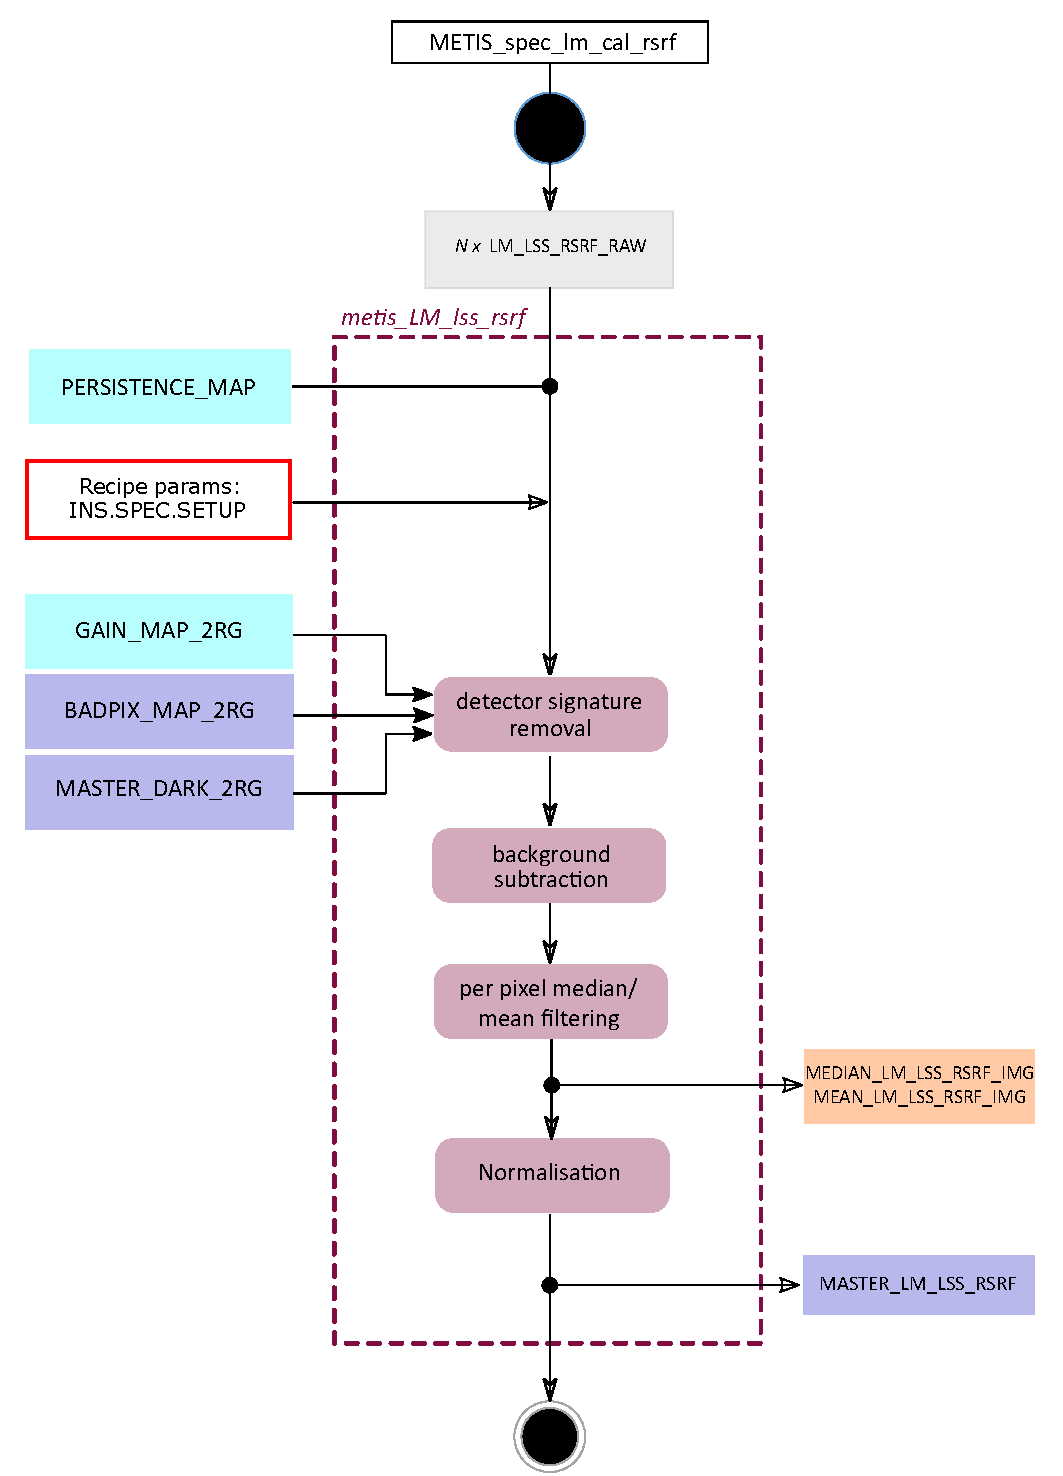
\includegraphics[width=0.5\textheight]{figures/metis_lm_lss_rsrf_v0.82.pdf}
  \caption[Recipe: \REC{metis_LM_lss_rsrf}]{\REC{metis_LM_lss_rsrf} --
    Recipe workflow to create the spectroscopic flatfield by means of the \ac{RSRF}.}
  \label{Fig:rec_lm_lss_rsrf}
\end{figure}

\begin{recipedef}
Name:		& \hyperref[rec:metis_lm_lss_rsrf]{\REC{metis_LM_lss_rsrf}}  \\
Purpose:	& Spectroscopic flatfielding with \ac{RSRF} \\
Type:		& Calibration\\
Requirements: & None \\
Templates:           & \TPL{METIS_spec_lm_cal_rsrf} \\
Input data:     & $N\times$ \hyperref[dataitem:lm_lss_rsrf_raw]{\RAW{LM_LSS_RSRF_RAW}} \\
                & \hyperref[dataitem:persistence_map]{\EXTCALIB{PERSISTENCE_MAP}}  \\
                & \hyperref[dataitem:gain_map_lm]{\STATCALIB{GAIN_MAP_LM}}  \\
                & \hyperref[dataitem:badpix_map_lm]{\PROD{BADPIX_MAP_LM}}  \\
                & \hyperref[dataitem:master_dark_lm]{\PROD{MASTER_DARK_LM}}  \\
Parameters: 	& TBD\\
Algorithm:      & subtract master \ac{WCU} "OFF" frame from illumination frame (done on individual images)\\
                & median/mean filtering of subtracted images\\
                & division by blackbody spectrum\\
                & normalisation to achieve \ac{RSRF}\\
Output data:	& \hyperref[dataitem:master_lm_lss_rsrf]{\PROD{MASTER_LM_LSS_RSRF}} (\FITS{PRO.CATG=MASTER_LM_LSS_RSRF}): \\
                & \hyperref[dataitem:median_lm_lss_rsrf_img]{\PROD{MEDIAN_LM_LSS_RSRF_IMG}}\\
                & \hyperref[dataitem:mean_lm_lss_rsrf_img]{\PROD{MEAN_LM_LSS_RSRF_IMG}}\\
Expected accuracies: & 3\% (cf. \cite{METIS-calibration_plan} and \cite{METIS_calerrbudget})\\
QC1 parameters: & \hyperref[qc:lmlssrsrfmeanlevel]{\QC{QC LM LSS RSRF MEAN LEVEL}}: Mean level of the \ac{RSRF}\\
                & \hyperref[qc:lmlssrsrfmedianlevel]{\QC{QC LM LSS RSRF MEDIAN LEVEL}}: Median level of the \ac{RSRF}\\
                & \hyperref[qc:lmlssrsrfintordrlevel]{\QC{QC LM LSS RSRF INTORDR LEVEL}}: Flux level of the interorder background\\
                & \hyperref[qc:lmlssrsrfnormstdev]{\QC{QC LM LSS RSRF NORM STDEV}}: Standard deviation of the normalised \ac{RSRF}\\
                & \hyperref[qc:lmlssrsrfnormsnr]{\QC{QC LM LSS RSRF NORM SNR}}: \ac{SNR} of the normalised \ac{RSRF}\\
                & more TBD\\
\end{recipedef}
\clearpage

%------------------------------------------------------------------------------------------------------------------
\subsubsection{LM-LSS Order detection \REC{metis_LM_lss_trace}:}\label{rec:metis_lm_lss_trace}
The recipe \hyperref[rec:metis_lm_lss_trace]{\REC{metis_LM_lss_trace}} aims at detecting the orders and a polynomial fitting of the order locations (see \cite{pis02} and \cite{pis21} for details on the algorithms). The detection and polynomial fitting is based on flatfield frames taken through a pinhole mask, which leads to individual pinhole traces along the entire dispersion direction.

\begin{figure}[ht]
  \centering
  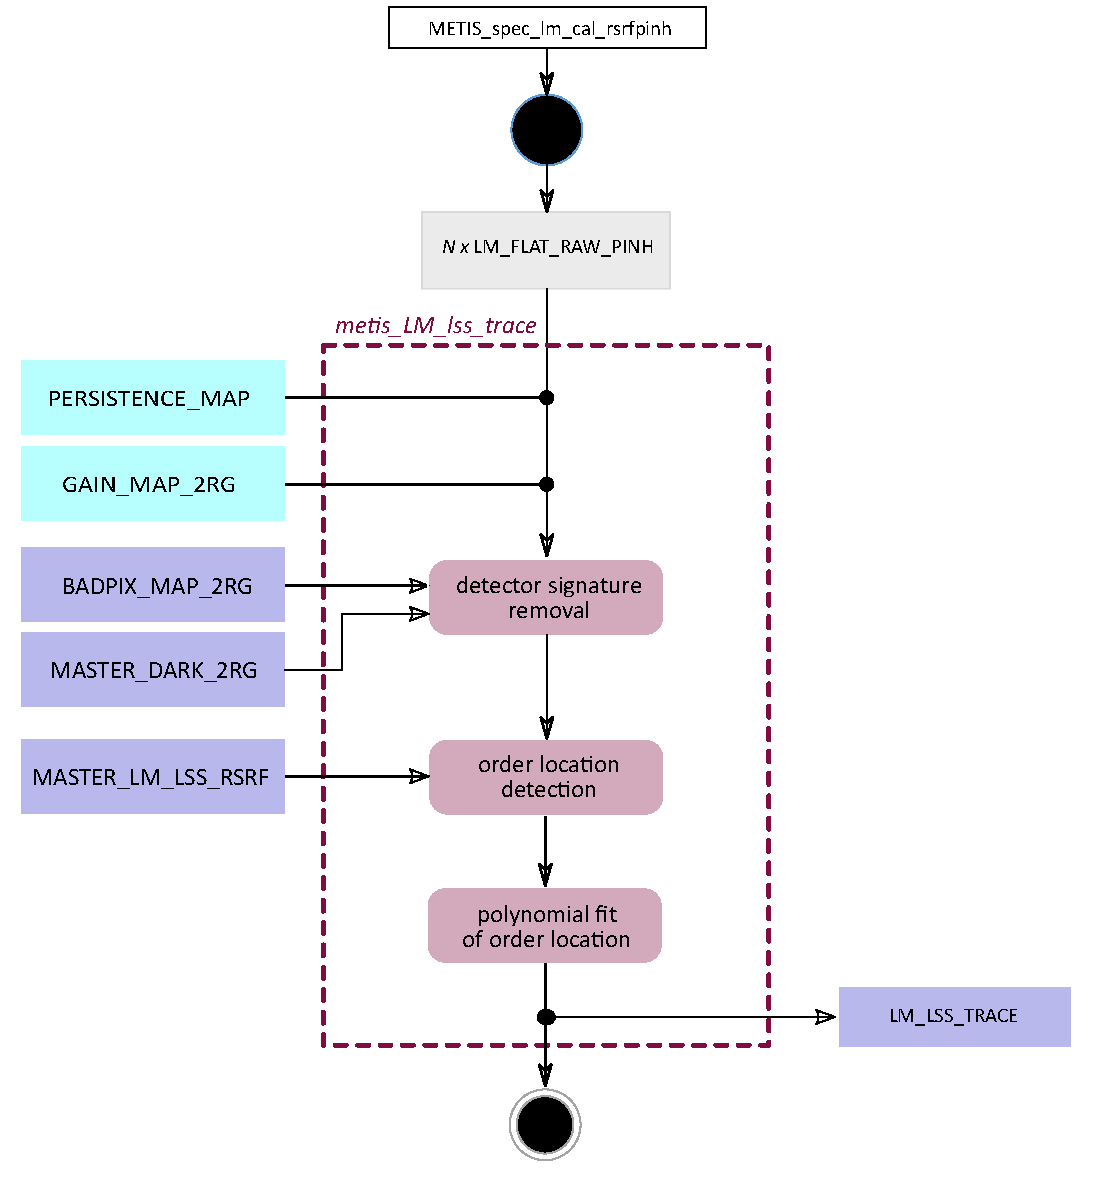
\includegraphics[width=0.5\textheight]{figures/metis_lm_lss_trace_v0.82.pdf}
  \caption[Recipe: \REC{metis_LM_lss_trace}]{\REC{metis_LM_lss_trace} --
    Detection and polynomial fitting of the order location.}
  \label{Fig:rec_lm_lss_wtrace}
\end{figure}

\begin{recipedef}
Name:		&  \hyperref[rec:metis_lm_lss_trace]{\REC{metis_LM_lss_trace}} \\
Purpose:	& Detection of order location \\
Type:		& Calibration\\
Requirements: & None \\
Templates:           & \TPL{METIS_spec_lm_cal_InternalWave}  \\
Input data:     & $N\times$ \hyperref[dataitem:lm_lss_rsrf_pinh_raw]{\RAW{LM_LSS_RSRF_PINH_RAW}} \\
                & \hyperref[dataitem:persistence_map]{\EXTCALIB{PERSISTENCE_MAP}}  \\
                & \hyperref[dataitem:gain_map_lm]{\STATCALIB{GAIN_MAP_LM}}  \\
                & \hyperref[dataitem:badpix_map_lm]{\PROD{BADPIX_MAP_LM}}  \\
                & \hyperref[dataitem:master_dark_lm]{\PROD{MASTER_DARK_LM}}  \\
                & \hyperref[dataitem:master_lm_lss_rsrf]{\PROD{MASTER_LM_LSS_RSRF}} \\
Parameters: 	& polynomial degree\\
Algorithm:      & Detection of the order edges\\
                & Polynomial fitting\\
Output data:	& \hyperref[dataitem:lm_lss_trace]{\PROD{LM_LSS_TRACE}} (\FITS{PRO.CATG=LM_LSS_TRACE}): Polynomial coefficients\\
Expected accuracies: & (TBD)\\
QC1 parameters: & \hyperref[qc:lmlsstracelpolydeg]{\QC{QC LM LSS TRACE LPOLYDEG}}: Degree of the polynomial fit of the left order edge\\
                & \hyperref[qc:lmlsstracelcoeffi]{\QC{QC LM LSS TRACE LCOEFF<i>}}: $i$-th coefficient of the polynomial of the left order edge\\
                & \hyperref[qc:lmlsstracerpolydeg]{\QC{QC LM LSS TRACE RPOLYDEG}}: Degree of the polynomial fit of the right order edge\\
                & \hyperref[qc:lmlsstracercoeffi]{\QC{QC LM LSS TRACE RCOEFF<i>}}: $i$-th coefficient of the polynomial of the right order edge\\
                & \hyperref[qc:lmlsstraceintrordrlevel]{\QC{QC LM LSS TRACE INTORDR LEVEL}}: Flux level of the interorder background\\
                & more TBD\\
\end{recipedef}

\clearpage
%------------------------------------------------------------------------------------------------------------------
\subsubsection{LM-LSS wavelength calibration recipe \REC{metis_LM_lss_wave}:}\label{rec:metis_lm_lss_wave}
This recipe aims at determining the first guess of the wavelength calibration on basis of the \ac{WCU} laser sources (c.f. \cite{METIS-calibration_plan}). Therefore the first steps are the removal of the detector signature of the \FITS{LM_WAVE_RAW} frames by applying the master calibration files derived in the previous steps, following by the background subtraction (if needed, TBD) and the application of the RSRF. The distortion of the lines (i.e. possible tilt, curvature,...) and the wavelength solution is determined by the algorithm developed by Piskunov et al. (\cite{pis02}, \cite{pis21}). The reference frame is defined by the laser line catalogue (\hyperref[dataitem:laser_tab]{\STATCALIB{LASER_TAB}}).

 This is in compliance with \REQ{METIS-6074}.

\begin{figure}[ht]
  \centering
  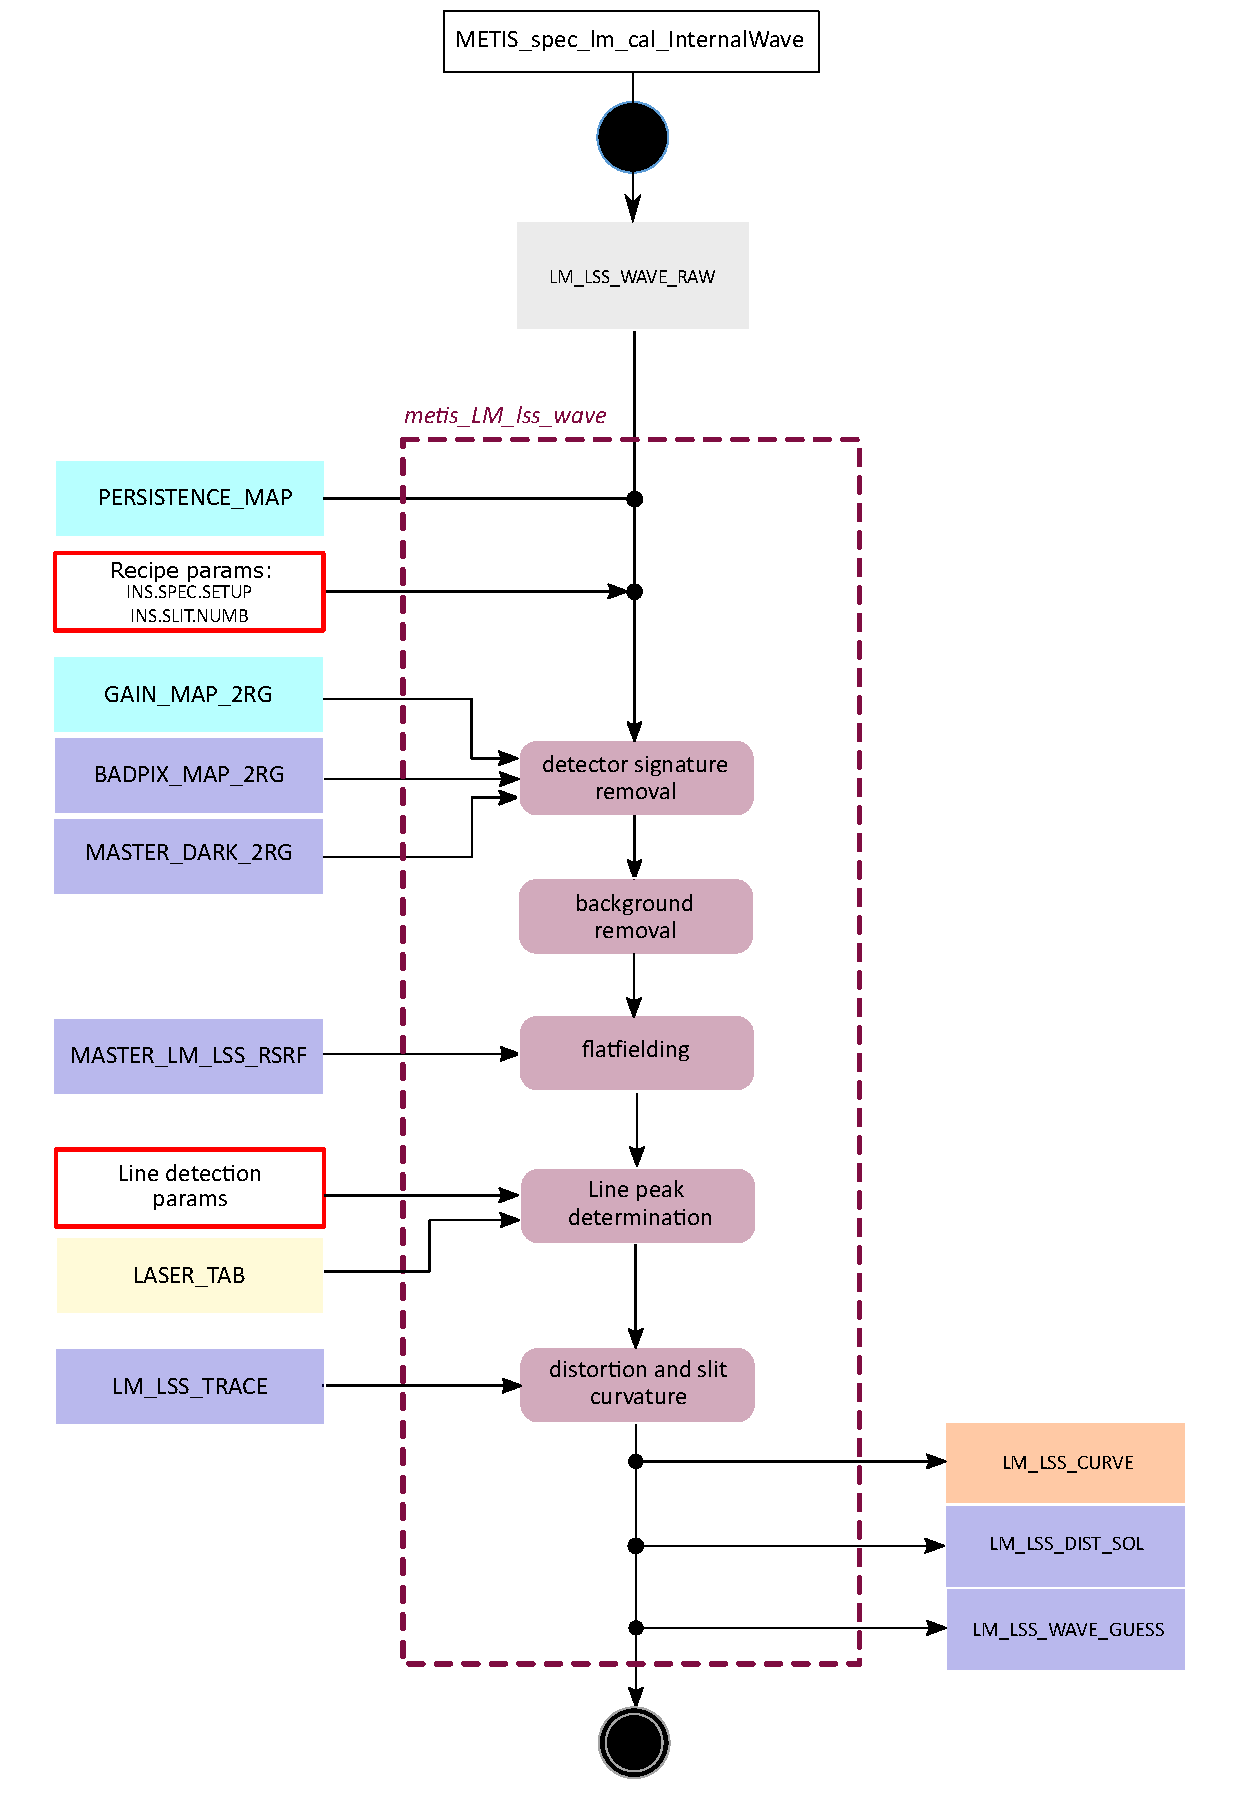
\includegraphics[width=0.5\textheight]{figures/metis_lm_lss_wave_v0.82.pdf}
  \caption[Recipe: \REC{metis_LM_lss_wave}]{\REC{metis_LM_lss_wave} --
    Creation of the LM LSS master wavelength correction.}
  \label{Fig:rec_lm_lss_trace}
\end{figure}
\clearpage

\begin{recipedef}
Name:		& \hyperref[rec:metis_lm_lss_wave]{\REC{metis_LM_lss_wave}} \\
Purpose:	& Wavelength calibration \\
Type:		& Calibration\\
Requirements: & METIS-6084, METIS-1371, METIS-6074 \\
Templates:           & \TPL{METIS_spec_lm_cal_internalwave}, \\
Input data: 	& \hyperref[dataitem:lm_lss_wave_raw]{\RAW{LM_LSS_WAVE_RAW}}\\
                & \hyperref[dataitem:persistence_map]{\EXTCALIB{PERSISTENCE_MAP}}  \\
                & \hyperref[dataitem:gain_map_lm]{\STATCALIB{GAIN_MAP_LM}}  \\
                & \hyperref[dataitem:badpix_map_lm]{\PROD{BADPIX_MAP_LM}}  \\
                & \hyperref[dataitem:master_dark_lm]{\PROD{MASTER_DARK_LM}}  \\
                & \hyperref[dataitem:master_lm_lss_rsrf]{\PROD{MASTER_LM_LSS_RSRF}} \\
                & \hyperref[dataitem:lm_lss_trace]{\PROD{LM_LSS_TRACE}} \\
                & \hyperref[dataitem:laser_tab]{\STATCALIB{LASER_TAB}} \\
                % & \hyperref[dataitem:ref_airg_cat]{\STATCALIB{REF_AIRG_CAT}} \\
Parameters: 	& (TBD)\\
Algorithm:      & Application of detector master calibration files\\
                & Determination and application of the distortion correction\\
                & Determination of the first guess of the wavelength solution by polynomial fit of the detected laser source lines\\
Output data:	& \hyperref[dataitem:lm_lss_curve]{\PROD{LM_LSS_CURVE}} (\FITS{PRO.CATG=LM_LSS_CURVE}): Curvature \\
                & \hyperref[dataitem:lm_lss_dist_sol]{\PROD{LM_LSS_DIST_SOL}} (\FITS{PRO.CATG=LM_LSS_DIST_SOL}): Distortion solution\\
                & \hyperref[dataitem:lm_lss_wave_guess]{\PROD{LM_LSS_WAVE_GUESS}} (\FITS{PRO.CATG=LM_LSS_WAVE_GUESS}): Wavelength first guess\\
Expected accuracies: & 1/5th of a pixel after post-processing (cf. \cite{METIS-calibration_plan})\\
QC1 parameters: & \hyperref[qc:lmlsswavepolydeg]{\QC{QC LM LSS WAVE POLYDEG}}: Degree of the first guess polynomial\\
                & \hyperref[qc:lmlsswavecoeffi]{\QC{QC LM LSS WAVE COEFF<i>}}: $i$-th coefficient of the polynomial\\
                & \hyperref[qc:lmlsswavenlines]{\QC{QC LM LSS WAVE NLINES}}: Number of detected (laser) lines; should be constant\\
                & \hyperref[qc:lmlsswavelinefwhmavg]{\QC{QC LM LSS WAVE LINEFWHMAVG}}: Average of the \ac{FWHM} of the detected lines (should be widely constant)\\
                & \hyperref[qc:lmlsswaveinterordrlevel]{\QC{QC LM LSS WAVE INTORDR LEVEL}}: Flux level of the interorder background\\
                & more TBD: e.g. QC params for distortion determination and correction\\
\end{recipedef}

\clearpage
%------------------------------------------------------------------------------------------------------------------
\subsubsection{LM-LSS standard star calibration recipe \REC{metis_LM_lss_std}:}\label{rec:metis_lm_lss_std}
\TODO{Finish following text} 

This recipe aims at processing standard stars used for the absolute flux calibration and (optionally) for the telluric feature removal: As first step the detector master calibration files derived previously are applied followed by the background subtraction, if needed the distortion correction (\hyperref[dataitem:lm_lss_dist_sol]{\PROD{LM_LSS_DIST_SOL}}), and
the wavelength calibration by means of the first guess solution (\hyperref[dataitem:lm_lss_wave_guess]{\PROD{LM_LSS_WAVE_GUESS}}) and the telluric sky lines (c.f. Sect.\,8.5 in \cite{DRLS}). Then the recipe removes sky background, extracts the standard star spectrum object and collapses the 2D to 1D spectra. To better compare the corresponding model spectrum a telluric correction is required. This is done by means of the standard star observations itself or (optionally) with \texttt{molecfit}.\\
It is on the user's decision whether the standard star is used for the absolute flux calibration only, or also used for the telluric correction of the science target.

As one needs to determine the stellar continuum regions, a telluric correction is required to increase these regions. This can be done either by applying a fairly simple telluric correction in an automated way to the standard star spectrum. In case the the user decides to use the standard star also for the telluric correction, a transmission function is derived from that in the "classical" way (cf. Section~\ref{sssec:tecllcorrclassic}), which will be optionally used for the telluric correction also for the science target. This star spectrum can also be optionally used for the wavelength solution and for the flux calibration, if the \ac{TSS} is suited for that. The response curve is obtained by comparing the extracted spectrum with a model and/or another reference spectrum of the standard star. Currently it is foreseen to use the same standard stars as in \ac{CRIRES}/CRIRES+ and \ac{VISIR}. It is under investigation whether more stars are needed.
\begin{figure}[ht]
  \centering
  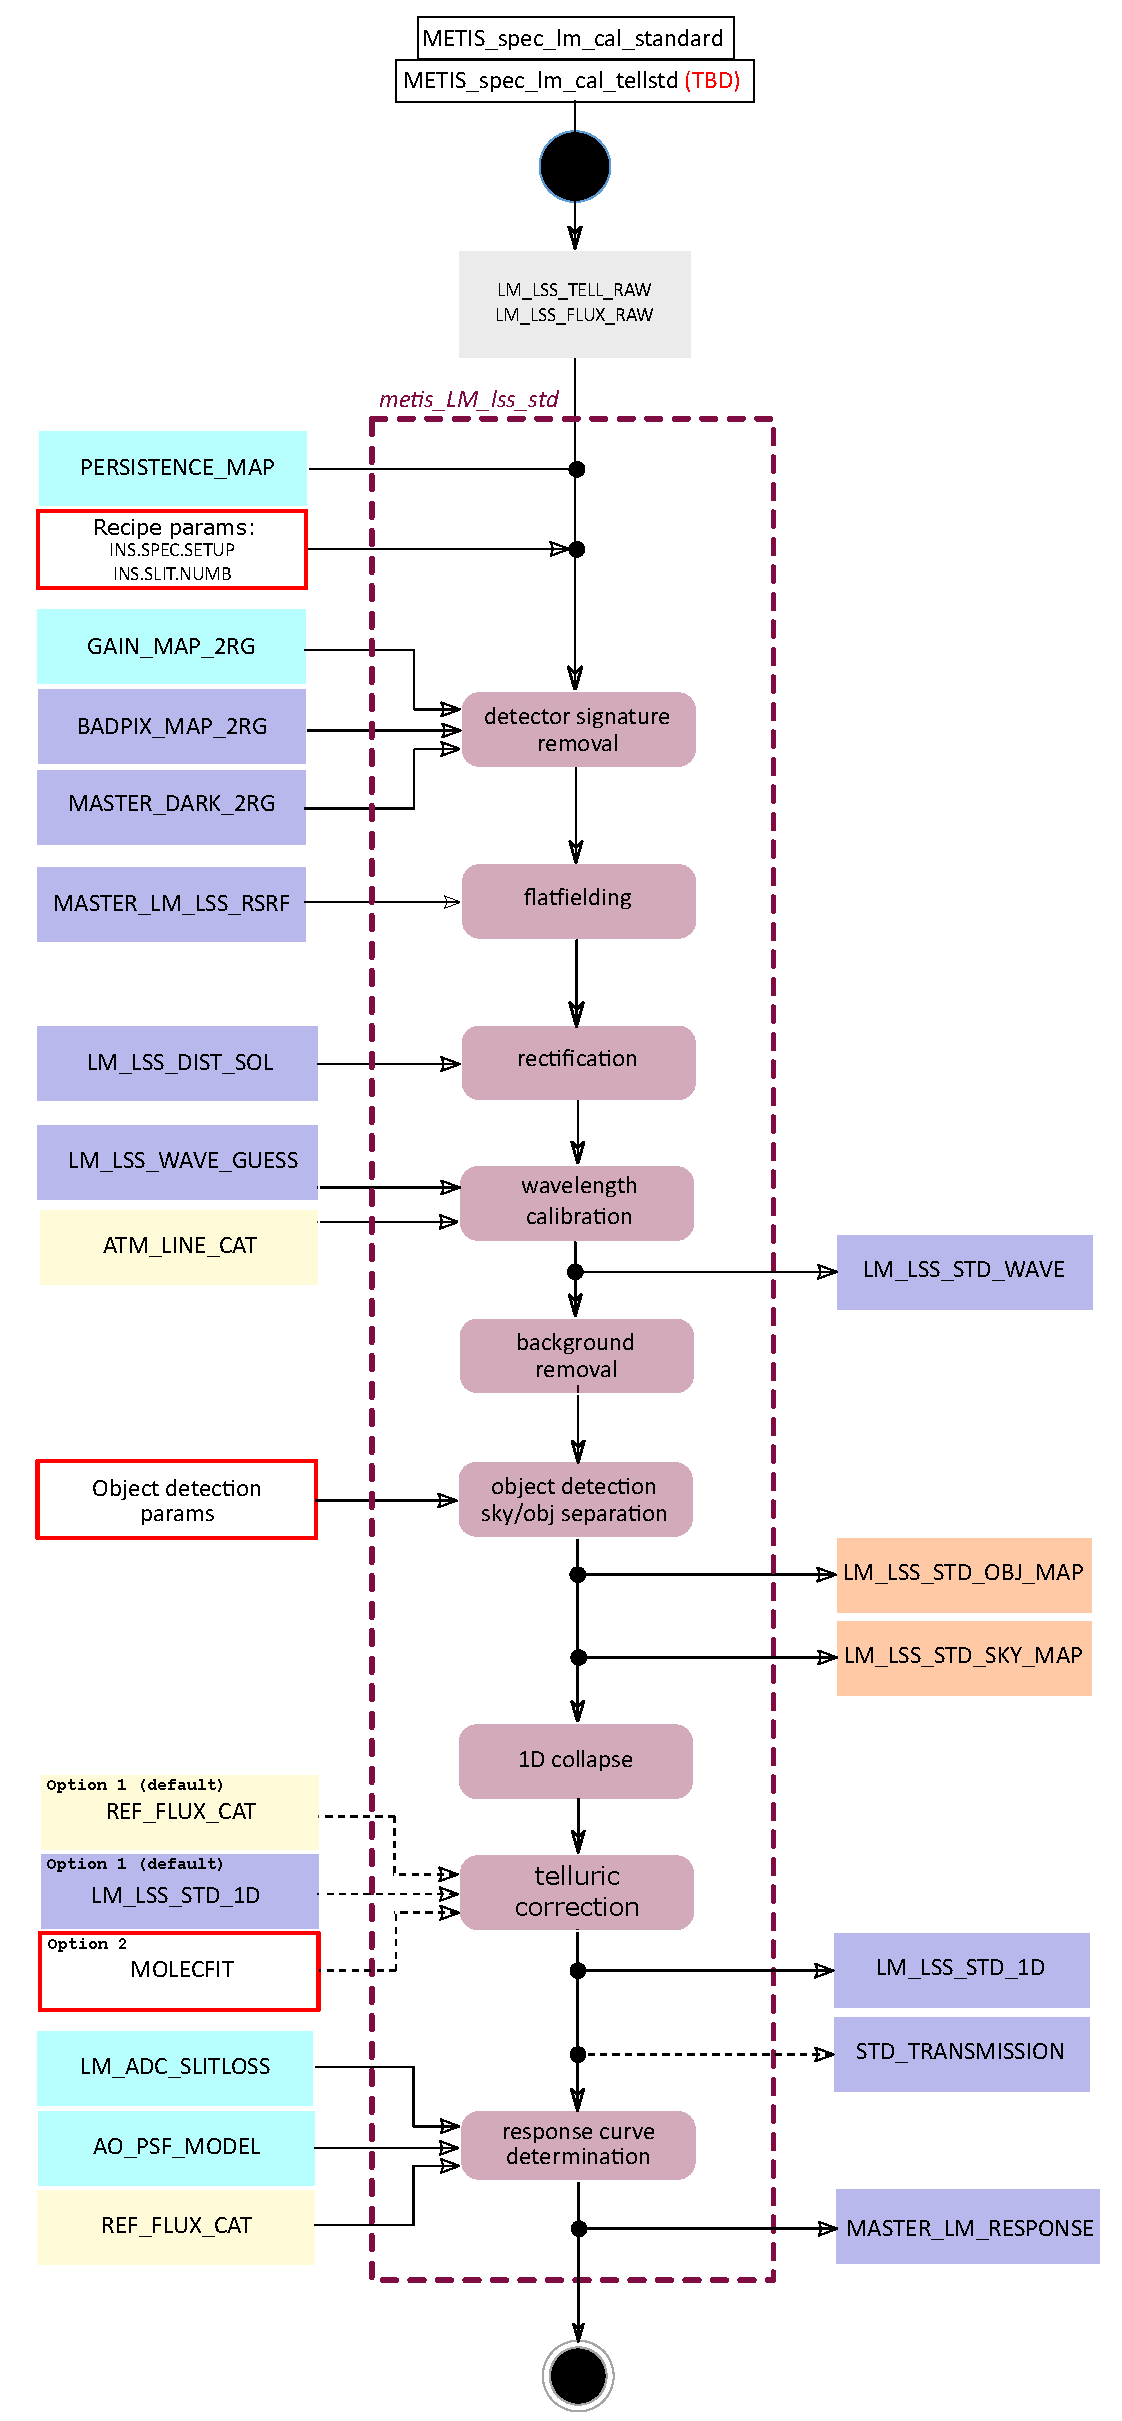
\includegraphics[width=0.4\textheight]{figures/metis_lm_lss_std_v0.82.pdf}
  \caption[Recipe: \REC{metis_LM_lss_std}]{\REC{metis_LM_lss_std} --
    Calibration recipe for processing standard stars for (combined) telluric and  spectro-photometric calibration.}
  \label{Fig:rec_lm_lss_flux1}
\end{figure}
%\begin{figure}[ht]
%  \centering
%  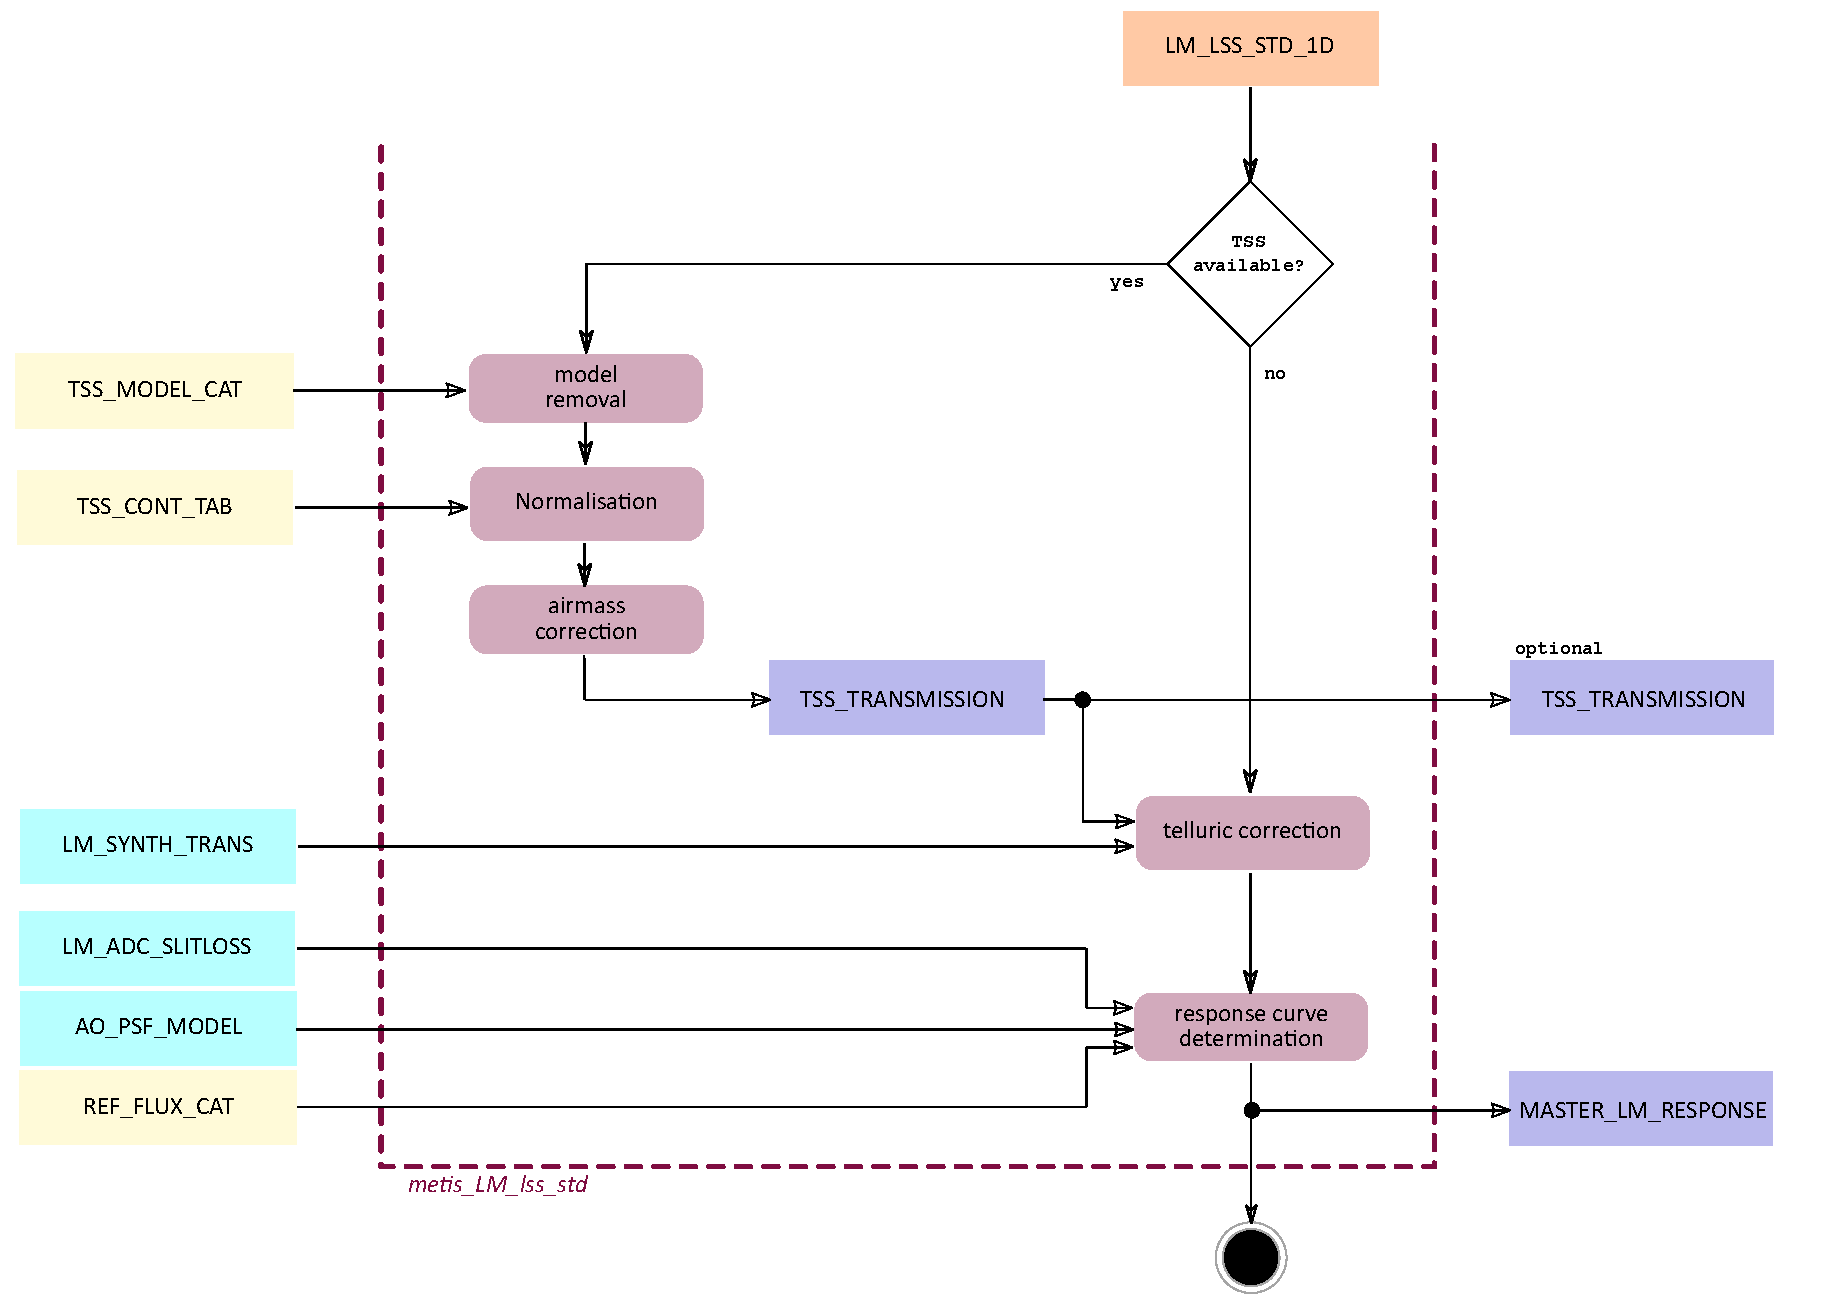
\includegraphics[width=0.6\textheight]{figures/metis_lm_lss_std_v0.8_part_2.pdf}
%  \caption[Recipe: \REC{metis_LM_lss_std}]{\REC{metis_LM_lss_std} --
%    Part 2 of the calibration recipe for processing spectrophotometric and telluric standard stars.}
%  \label{Fig:rec_lm_lss_flux2}
%\end{figure}
\clearpage
\begin{recipedef}
Name:		& \hyperref[rec:metis_lm_lss_std]{\REC{metis_LM_lss_std}} \\
Purpose:	& Flux calibration \\
Type:		& Calibration\\
Requirements: & METIS-6084, METIS-6074 \\
Templates:           & \TPL{METIS_spec_lm_cal_standard}\\
Input data: 	& \hyperref[dataitem:lm_lss_flux_raw]{\RAW{LM_LSS_FLUX_RAW}}\\
                & \hyperref[dataitem:persistence_map]{\EXTCALIB{PERSISTENCE_MAP}}  \\
                & \hyperref[dataitem:gain_map_lm]{\STATCALIB{GAIN_MAP_LM}}  \\
                & \hyperref[dataitem:badpix_map_lm]{\PROD{BADPIX_MAP_LM}}  \\
                & \hyperref[dataitem:master_dark_lm]{\PROD{MASTER_DARK_LM}}  \\
                & \hyperref[dataitem:master_lm_lss_rsrf]{\PROD{MASTER_LM_LSS_RSRF}} \\
                & \hyperref[dataitem:lm_lss_dist_sol]{\PROD{LM_LSS_DIST_SOL}} \\
                & \hyperref[dataitem:lm_lss_wave_guess]{\PROD{LM_LSS_WAVE_GUESS}} \\
                & \hyperref[dataitem:ao_psf_model]{\EXTCALIB{AO_PSF_MODEL}} \\
                & \hyperref[dataitem:atm_line_cat]{\EXTCALIB{ATM_LINE_CAT}} \\
%                & \hyperref[dataitem:tss_model_cat]{\STATCALIB{TSS_MODEL_CAT}}\\
%                & \hyperref[dataitem:tss_cont_tab]{\STATCALIB{TSS_CONT_TAB}}\\
                & \hyperref[dataitem:lm_adc_slitloss]{\STATCALIB{LM_ADC_SLITLOSS}}\\
                & \hyperref[dataitem:lm_synth_trans]{\STATCALIB{LM_SYNTH_TRANS}}\\
                & \hyperref[dataitem:ref_std_cat]{\STATCALIB{REF_STD_CAT}} \\
Parameters: 	& (TBD)\\
Algorithm:      & Application of master calibration files\\
                & Background removal\\
                & Determination and application of the distortion correction\\
                & Determination and application of the wavelength solution\\
                & Identifying/separatiing sky/object pixels\\
                & Removing sky lines: Creation and Subtraction of 2D sky\\
                & Collapsing 2D to 1D spectrum, (see Fig.\,\ref{Fig:rec_lm_lss_sci})\\
                & Determination and application of response curve\\
Output data:	& \hyperref[dataitem:lm_lss_std_obj_map]{\PROD{LM_LSS_STD_OBJ_MAP}}: Pixel map of object pixels\\
            	& \hyperref[dataitem:lm_lss_std_sky_map]{\PROD{LM_LSS_STD_SKY_MAP}}: Pixel map of sky pixels\\
              	& \hyperref[dataitem:lm_lss_std_1d]{\PROD{LM_LSS_STD_1D}}: coadded, wavelength calibrated, collapsed 1D spectrum\\
              	& \hyperref[dataitem:lm_lss_std_wave]{\PROD{LM_LSS_STD_WAVE}}: Wavelength solution derived from the \ac{STD} star (optional)\\
            	& \hyperref[dataitem:std_transmission]{\PROD{STD_TRANSMISSION}}: Transmission function derived by means of the \ac{STD} (optional)\\        
                & \hyperref[dataitem:master_lm_response]{\PROD{MASTER_LM_RESPONSE}}: response function \\
Expected accuracies: & 10\% over an atmospheric band (ESO Req. R-MET-107)\\
            & $<30$\% absolute line flux accuracy (R-MET-107)\\
            & $<5$\% absolute flux calibration (R-MET-82)\\
QC1 parameters: & \hyperref[qc:lmlssstdbackgdmean]{\QC{QC LM LSS STD BACKGD MEAN}}: Mean value of background\\
                & \hyperref[qc:lmlssstdbackgdmedian]{\QC{QC LM LSS STD BACKGD MEDIAN}}: Median value of background\\
                & \hyperref[qc:lmlssstdbackgdstdev]{\QC{QC LM LSS STD BACKGD STDEV}}: Standard deviation value of background\\
                & \hyperref[qc:lmlssstdsnr]{\QC{QC LM LSS STD SNR}}: Signal-to-noise ration of flux standard star spectrum\\
                & \hyperref[qc:lmlssstdsnrnoise]{\QC{QC LM LSS STD SNRNOISE}}: Noise level of flux standard star spectrum\\
                & \hyperref[qc:lmlssstdfwhm]{\QC{QC LM LSS STD FWHM}}: FWHM of flux standard spectrum\\
                & \hyperref[qc:lmlssfluxintrordravglevel]{\QC{QC LM LSS FLUX INTORDR LEVEL}}: Flux level of the interorder background\\
                & \hyperref[qc:lmlssfluxlevel]{\QC{QC LM LSS FLUX AVGLEVEL}}: Average level of the standard star flux \\
                & \hyperref[qc:lmlssfluxwavecaldevmean]{\QC{QC LM LSS FLUX WAVECAL DEVMEAN}}: Mean deviation from the
                  wavelength reference frame (TBDef)\\
                & \hyperref[qc:lmlssfluxwavecalfwhm]{\QC{QC LM LSS FLUX WAVECAL FWHM}}: Measured FWHM of lines\\
                & \hyperref[qc:lmlssfluxwavecalnident]{\QC{QC LM LSS FLUX WAVECAL NIDENT}}: Number of identified lines\\
                & \hyperref[qc:lmlssfluxwavecalnmatch]{\QC{QC LM LSS FLUX WAVECAL NMATCH}}: Number of lines matched between
                    catalogue and spectrum\\
                & \hyperref[qc:lmlssfluxwavecalpolydeg]{\QC{QC LM LSS FLUX WAVECAL POLYDEG}}: Degree of the polynomial\\
                & \hyperref[qc:lmlssfluxwavecalpolycoeffn]{\QC{QC LM LSS FLUX WAVECAL POLYCOEFF\<n\>}}: $n$-th coefficient of the polynomial\\
                & \hyperref[qc:lmlssfluxstdsnr]{\QC{QC LM LSS FLUX STDSNR}}: Signal-to-noise ration of flux standard star spectrum\\
                & \hyperref[qc:lmlssfluxsnrnoise]{\QC{QC LM LSS FLUX SNRNOISE}}: Noise level of flux standard star spectrum\\
                & \hyperref[qc:lmlssfluxfwhm]{\QC{QC LM LSS FLUX FWHM}}: FWHM of flux standard spectrum\\
                & \hyperref[qc:lmlssfluxpsfloss]{\QC{QC LM LSS FLUX PSFLOSS}}: Fraction of AO induced slit losses (TBdef)\\
                & more TBD
\end{recipedef}

\subsubsection{LM-LSS science reduction recipe \REC{metis_LM_lss_sci}:}\label{rec:metis_lm_lss_sci}
The science calibration recipe comprises the extraction of the object (i.e. separation of object/sky pixels), removing the sky lines, the application of the response curve previously defined, the 2D to 1D collapse and the co-addition. In contrast to the flux standard star reduction, the telluric correction on the science data is done in a dedicated recipe afterwards to achieve best quality for the correction.
\begin{figure}[ht]
  \centering
  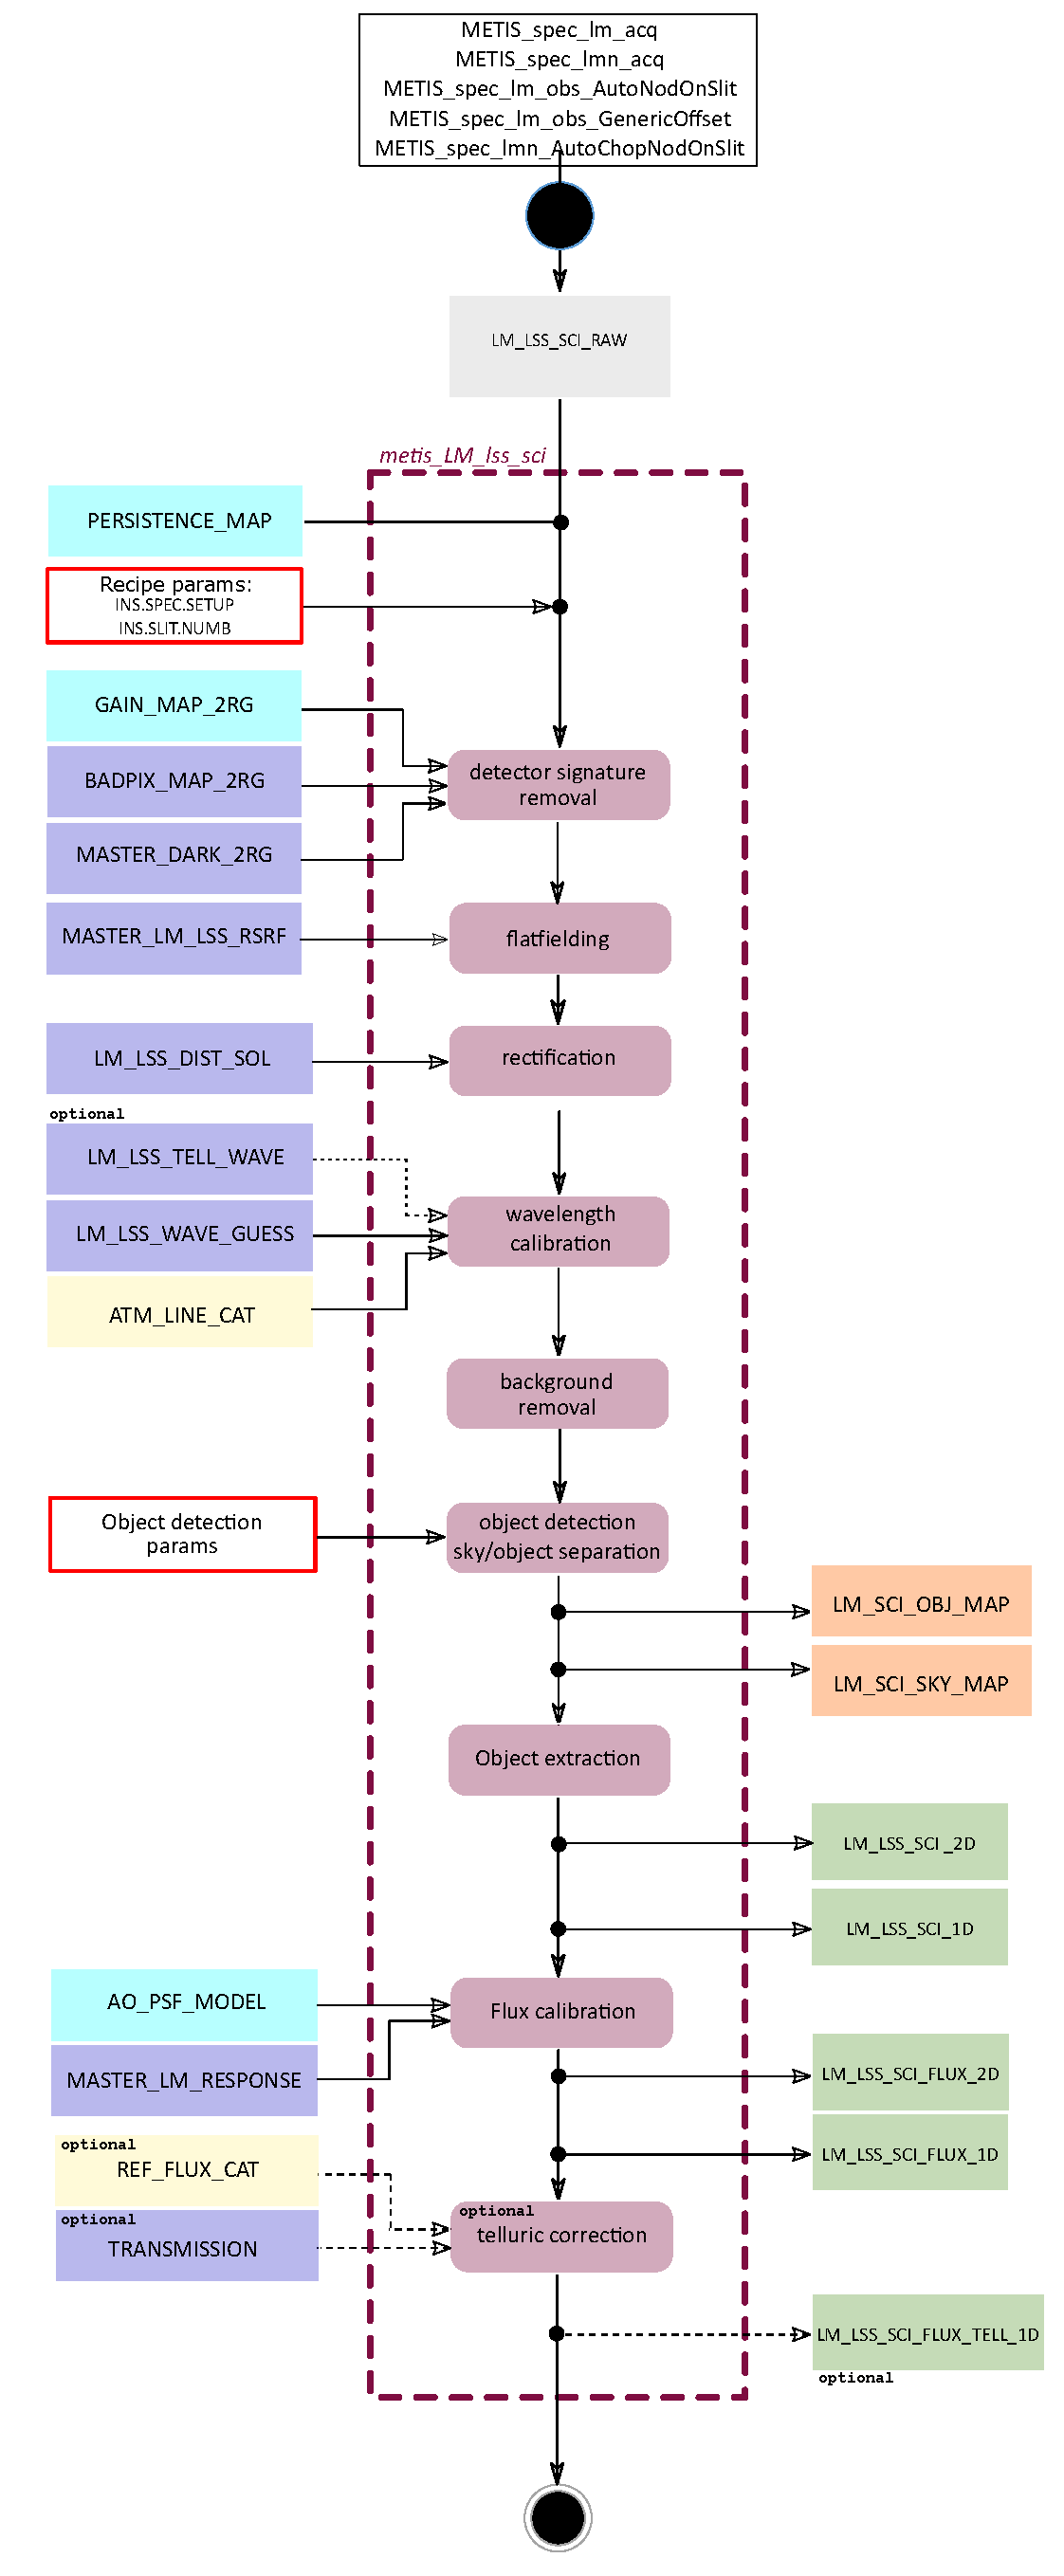
\includegraphics[width=0.37\textheight]{figures/metis_lm_lss_sci_v0.82.pdf}
  \caption[Recipe: \REC{metis_LM_lss_sci}]{\REC{metis_LM_lss_sci} --
    Science reduction recipe.}
  \label{Fig:rec_lm_lss_sci}
\end{figure}
\clearpage

\begin{recipedef}
Name:		& \hyperref[rec:metis_lm_lss_sci]{\REC{metis_LM_lss_sci}} \\
Purpose:    & Science data calibration\\
Type:		& Science reduction\\
Requirements: & METIS-6084 \\
Templates:           & \TPL{METIS_spec_lm_acq}, \\
                & \TPL{METIS_spec_lm_obs_AutoNodOnSlit}, \\
                & \TPL{METIS_spec_lm_obs_GenericOffset} \\
                & \TPL{METIS_spec_lm_cal_SlitAdc}\\
Input data: 	& \hyperref[dataitem:lm_lss_sci_raw]{\RAW{LM_LSS_SCI_RAW}}\\
                & \hyperref[dataitem:persistence_map]{\EXTCALIB{PERSISTENCE_MAP}}  \\
                & \hyperref[dataitem:gain_map_lm]{\STATCALIB{GAIN_MAP_LM}}  \\
                & \hyperref[dataitem:badpix_map_lm]{\PROD{BADPIX_MAP_LM}}  \\
                & \hyperref[dataitem:master_dark_lm]{\PROD{MASTER_DARK_LM}}  \\
                & \hyperref[dataitem:master_lm_lss_rsrf]{\PROD{MASTER_LM_LSS_RSRF}} \\
                & \hyperref[dataitem:lm_lss_dist_sol]{\PROD{LM_LSS_DIST_SOL}} \\
                & \hyperref[dataitem:lm_lss_wave_guess]{\PROD{LM_LSS_WAVE_GUESS}} \\
                & \hyperref[dataitem:atm_line_cat]{\EXTCALIB{ATM_LINE_CAT}} \\
                & \hyperref[dataitem:lm_adc_slitloss]{\STATCALIB{LM_ADC_SLITLOSS}}\\
            	& \hyperref[dataitem:std_transmission]{\PROD{STD_TRANSMISSION}} (optional)\\             
                %& \hyperref[dataitem:ao_psf_model]{\EXTCALIB{AO_PSF_MODEL}} \\
                %& \hyperref[dataitem:lsf_kernel]{\STATCALIB{LSF_KERNEL}}\\
                & \hyperref[dataitem:master_lm_response]{\PROD{MASTER_LM_RESPONSE}} \\
Parameters: 	& (TBD)\\
Algorithm:      & Application of the detector master calib files\\
                & wavelength calibration \\
                & Identifying/separatiing sky/object pixels\\
                & Removing sky lines: Creation and Subtraction of 2D sky\\
                & Coaddition of individual object spectra of one OB\\
                & Collapsing 2D to 1D spectrum, (see Fig.\,\ref{Fig:rec_lm_lss_sci})\\
                & Application of the response function (flux calibration) \\
Output data:	& \hyperref[dataitem:lm_lss_sci_obj_map]{\PROD{LM_LSS_SCI_OBJ_MAP}}: Pixel map of object pixels\\
            	& \hyperref[dataitem:lm_lss_sci_sky_map]{\PROD{LM_LSS_SCI_SKY_MAP}}: Pixel map of sky pixels\\
            	& \hyperref[dataitem:lm_lss_sci_2d]{\PROD{LM_LSS_SCI_2D}}: coadded, wavelength calibrated 2D spectrum\\
                & (\FITS{PRO_CATG}: \FITS{LM_LSS_2d_coadd_wavecal}) \\
                & \hyperref[dataitem:lm_lss_sci_1d]{\PROD{LM_LSS_SCI_1D}}: coadded, wavelength calibrated 1D spectrum\\
                & (\FITS{PRO_CATG}: \FITS{LM_LSS_1d_coadd_wavecal}) \\
                & \hyperref[dataitem:lm_lss_sci_flux_2d]{\PROD{LM_LSS_SCI_FLUX_2D}}: coadded, wavelength + flux calibrated 2D spectrum\\
                & (\FITS{PRO_CATG}: \FITS{LM_LSS_2d_coadd_wavecal}) \\
              	& \hyperref[dataitem:lm_lss_sci_flux_1d]{\PROD{LM_LSS_SCI_FLUX_1D}}: coadded, wavelength + flux 1D spectrum\\
                & (\FITS{PRO_CATG}: \FITS{LM_LSS_1d_coadd_wavecal}) \\
Expected accuracies: & (TBD)\\
QC1 parameters: & \hyperref[qc:lmlssscisnr]{\QC{QC LM LSS SCI SNR}}: Signal-to-noise ration of science spectrum\\
                & \hyperref[qc:lmlssscisnrnoise]{\QC{QC LM LSS SCI SNRNOISE}}: Noise level of science spectrum\\
                & \hyperref[qc:lmlssscifluxsnr]{\QC{QC LM LSS SCI FLUX SNR}}: Signal-to-noise ration of flux calibrated  science spectrum\\
                & \hyperref[qc:lmlssscifluxsnrnoise]{\QC{QC LM LSS SCI FLUX SNRNOISE}}: Noise level of flux calibrated science spectrum\\
                & \hyperref[qc:lmlsssciinterordrlevel]{\QC{QC LM LSS SCI INTORDR LEVEL}}: Flux level of the interorder background\\
                & \hyperref[qc:lmlsssciwavecaldevmean]{\QC{QC LM LSS SCI WAVECAL DEVMEAN}}: Mean deviation from the wavelength reference frame (TBDef)\\
                & \hyperref[qc:lmlsssciwavecalfwhm]{\QC{QC LM LSS SCI WAVECAL FWHM}}: Measured FWHM of lines\\
                & \hyperref[qc:lmlsssciwavecalnident]{\QC{QC LM LSS SCI WAVECAL NIDENT}}: Number of identified lines\\
                & \hyperref[qc:lmlsssciwavecalnmatch]{\QC{QC LM LSS SCI WAVECAL NMATCH}}: Number of lines matched between catalogue and spectrum\\
                & \hyperref[qc:lmlsssciwavecalpolydeg]{\QC{QC LM LSS SCI WAVECAL POLYDEG}}: Degree of the wavelength polynomial\\
                & \hyperref[qc:lmlsssciwavecalpolycoeffn]{\QC{QC LM LSS SCI WAVECAL POLYCOEFF\<n\>}}: $n$-th coefficient of the polynomial\\
                & more TBD\\
\end{recipedef}

\subsubsection{LM-LSS telluric correction recipe \REC{metis_LM_lss_mf_model}:}\label{rec:metis_lm_lss_mf_model}
The telluric correction will be done with the package \texttt{molecfit}\footnote{\url{https://www.eso.org/sci/software/pipelines/molecfit/molecfit-pipe-recipes.html}}. It is realised in three individual recipes, \hyperref[rec:metis_lm_lss_mf_model]{\REC{metis_LM_lss_mf_model}}, which calculates the best-fit model, \hyperref[rec:metis_lm_lss_mf_calctrans]{\REC{metis_LM_lss_mf_calctrans}}, which creates a synthetic transmission curve, and \hyperref[rec:metis_lm_lss_mf_correct]{\REC{metis_LM_lss_mf_correct}}, which performs the actual telluric correction by means of the synthetic transmission.

\begin{figure}[ht]
  \centering
  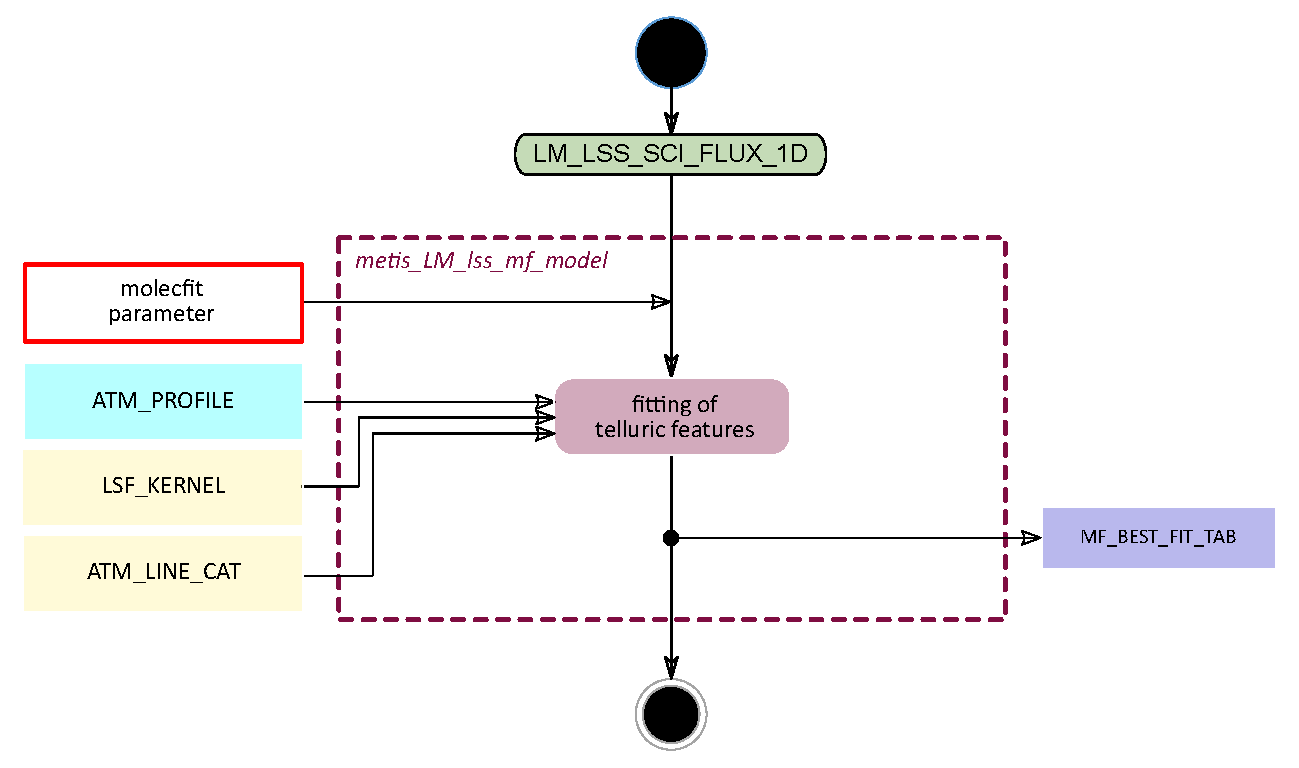
\includegraphics[width=0.5\textheight]{figures/metis_lm_lss_mf_model_v0.82.pdf}
  \caption[Recipe: \REC{metis_LM_lss_mf_model}]{\REC{metis_LM_lss_mf_model} --
    Recipe to achieve the best-fit for the calculation of the synthetic transmission curve for the telluric correction.}
  \label{Fig:rec_lm_lss_mf_model}
\end{figure}
\clearpage

\begin{recipedef}
Name:		& \hyperref[rec:metis_lm_lss_mf_model]{\REC{metis_LM_lss_mf_model}} \\
Purpose:	& Achieve the best fit for modelling the transmission curve to be applied as telluric correction \\
Type:		& Post-calibration\\
Requirements: & METIS-4051, METIS-6091 \\
Templates:           & None\\
Input data: 	& \hyperref[dataitem:lm_lss_sci_flux_1d]{\PROD{LM_LSS_SCI_FLUX_1D}}\\
                & \hyperref[dataitem:lsf_kernel]{\STATCALIB{LSF_KERNEL}} \\
                & \hyperref[dataitem:atm_profile]{\EXTCALIB{ATM_PROFILE}} \\
                & \hyperref[dataitem:atm_line_cat]{\EXTCALIB{ATM_LINE_CAT}} \\
Parameters: 	& \texttt{molecfit} parameters (c.f. \cite{molecfit})\\
Algorithm:      & Fit of telluric features visible in the science input spectrum\\
                & Determination of best-fit parameter set\\
Output data:	& \hyperref[dataitem:mf_best_fit_tab]{\PROD{MF_BEST_FIT_TAB}}: Table with best-fit parameters\\
Expected accuracies: & (TBD)\\
QC1 parameters: & cf. \cite{molecfit}\\
\end{recipedef}

\subsubsection{LM-LSS telluric correction recipe \REC{metis_LM_lss_mf_calctrans}:}\label{rec:metis_lm_lss_mf_calctrans}

\begin{figure}[ht]
  \centering
  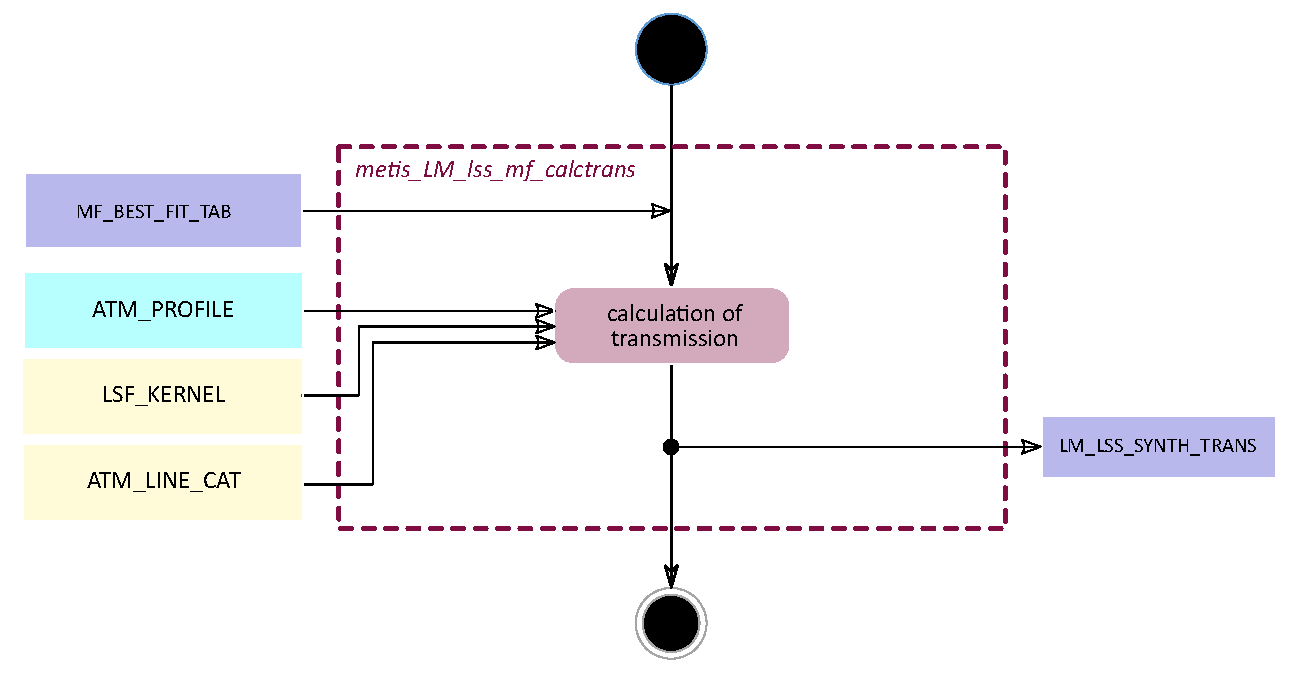
\includegraphics[width=0.5\textheight]{figures/metis_lm_lss_mf_calctrans_v0.82.pdf}
  \caption[Recipe: \REC{metis_LM_lss_mf_calctrans}]{\REC{metis_LM_lss_mf_calctrans} --
    Recipe to calculate the synthetic transmission to be applied as telluric correction.}
  \label{Fig:rec_lm_lss_mf_calctrans}
\end{figure}
\clearpage

\begin{recipedef}
Name:		& \hyperref[rec:metis_lm_lss_mf_calctrans]{\REC{metis_LM_lss_mf_calctrans}} \\
Purpose:	& Calculation of the synthetic transmission \\
Type:		& Post-calibration\\
Requirements: & METIS-4051, METIS-6091 \\
Templates:           & None\\
Input data: 	& \hyperref[dataitem:mf_best_fit_tab]{\PROD{MF_BEST_FIT_TAB}}: Table with best-fit parameters\\
                & \hyperref[dataitem:lsf_kernel]{\STATCALIB{LSF_KERNEL}} \\
                & \hyperref[dataitem:atm_profile]{\EXTCALIB{ATM_PROFILE}} \\
                & \hyperref[dataitem:atm_line_cat]{\EXTCALIB{ATM_LINE_CAT}} \\
Parameters: 	& \texttt{molecfit} parameters (c.f.  \cite{molecfit})\\
Algorithm:      & Calculate the entire transmission curve by means of the best-fit parameters\\
Output data:	& \hyperref[dataitem:lm_lss_synth_trans]{\PROD{LM_LSS_SYNTH_TRANS}}: synth. transmission\\
Expected accuracies: & (TBD)\\
QC1 parameters: & cf. \cite{molecfit}\\
\end{recipedef}

\subsubsection{LM-LSS telluric correction recipe \REC{metis_LM_lss_mf_correct}:}\label{rec:metis_lm_lss_mf_correct}

\begin{figure}[ht]
  \centering
  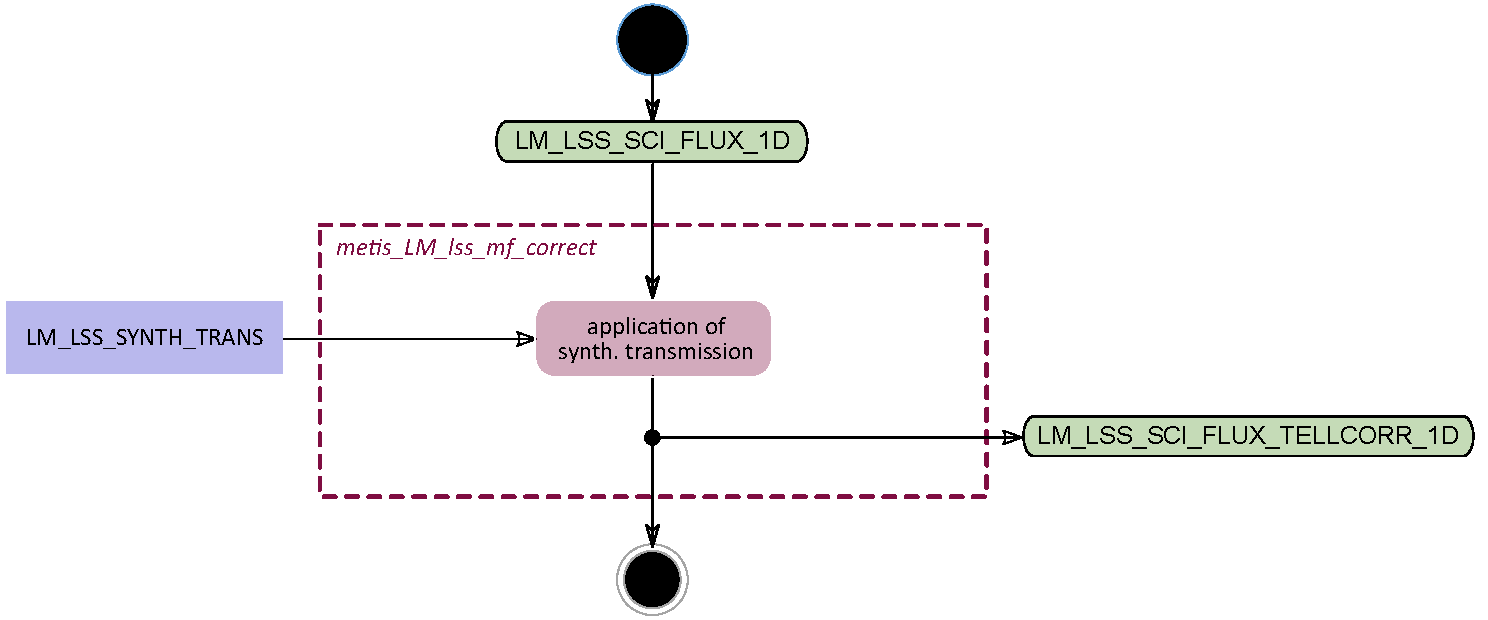
\includegraphics[width=0.5\textheight]{figures/metis_lm_lss_mf_correct_v0.82.pdf}
  \caption[Recipe: \REC{metis_LM_lss_mf_correct}]{\REC{metis_LM_lss_mf_correct} --
    Recipe to apply the telluric correction.}
  \label{Fig:rec_lm_lss_mf_correct}
\end{figure}
\clearpage

\begin{recipedef}
Name:		& \hyperref[rec:metis_lm_lss_mf_correct]{\REC{metis_LM_lss_mf_correct}} \\
Purpose:	& Apply the synthetic transmission to the science spectra \\
Type:		& Post-calibration\\
Requirements: & METIS-4051, METIS-6091 \\
Templates:           & None\\
Input data: 	& \hyperref[dataitem:lm_lss_sci_flux_1d]{\PROD{LM_LSS_SCI_FLUX_1D}}\\
                & \hyperref[dataitem:lm_lss_synth_trans]{\PROD{LM_LSS_SYNTH_TRANS}}\\
Parameters: 	& None\\
Algorithm:      & Apply telluric correction, i.e. divide the input science spectrum\\
                & by the synthetic transmission\\
Output data:	& \hyperref[dataitem:lm_lss_sci_flux_tellcorr_1d]{\PROD{LM_LSS_SCI_FLUX_TELLCORR_1D}}\\
Expected accuracies: & (TBD)\\
QC1 parameters: & cf. \cite{molecfit}\\
\end{recipedef}




\clearpage
\subsection{N-band long-slit spectroscopy recipes}
\label{ssec:recipes_lss_n}
A draft of the reduction cascade is shown in Figs.~\ref{Fig:NLssAssomap1} and \ref{Fig:NLssAssomap2}.% together with the data processing table (Tables~\ref{Tab:NLssDatProc1} and ~\ref{Tab:NLssDatProc2}). 
The first part aims to update the static calibration database, in particular the creation of the gain map (\REC{metis_det_lingain}) and the determination of the \ac{ADC} slitlosses (\REC{metis_n_adc_slitloss}). Both are executed only when an update is required, e.g. after a major instrument interention or on yearly basis. The second part comprises the basic calibrations, e.g. the dark correction and the spectroscopic flatfielding via \ac{RSRF}, followed by the third part, the main calibration steps, incorporating the wavelength calibration (by means of atmospheric lines visible in the respective spectra and the first guess wavelength solution created during \ac{AIT}) and the determination of the response curve for the flux calibration. Therefore the main step of the wavelength calibration is carried out in the recipes \REC{metis_N_lss_std} and \REC{metis_LM_lss_sci}. Finally, the telluric absorption correction is applied using the modelling approach with \texttt{molecfit}.
%------------------------------------------------------------------------------------------------------------------
%\subsubsection{Recipes \REC*{metis_det_lingain} and \REC*{metis_det_dark}}
These recipes aim for detector-specific calibrations and are therefore the same as in the imaging pipeline. Common detector calibrations are described in Section~\ref{Sec:detector_calibration}.\\
Note that the list of \ac{QC} parameters in the recipe descriptions will be extended whenever necessary.\\
%------------------------------------------------------------------------------------------------------------------
\subsubsection{\REC*{metis_det_lingain} and \REC*{metis_det_dark}: Linearity/Gain}
These recipes aim for detector-specific calibrations and are therefore the same as in the imaging pipeline. Common detector calibrations are described in Section~\ref{Sec:detector_calibration}.

%------------------------------------------------------------------------------------------------------------------
\subsubsection{\REC*{metis_N_adc_slitloss}: Slit loss determination}
The recipe \REC{metis_n_adc_slitloss} aims to determine the slit losses induced by atmospheric refraction. The recipe aims to create a table with slitlosses (\STATCALIB{N_ADC_SLITLOSS}), which is added to the static database and used in the recipes \REC{metis_N_lss_std}. This recipe is to be carried out only when an update of the database is needed. The algorithm and the workflow of the recipe to determine the slitlosses is given in Section~\ref{sssec:adc_slitlosses}, more information can be found in Section "Calibration of slit losses" in the Calibration Plan~\cite{METIS-calibration_plan}. 

%------------------------------------------------------------------------------------------------------------------
\subsubsection{\REC*{metis_N_lss_rsrf}:  Flatfielding}\label{rec:metis_n_lss_rsrf}
The recipe \REC{metis_N_lss_rsrf} aims to create a spectroscopic master flatfield for determining the pixel-to-pixel sensitivity and to enable the order location algorithm (\REC{metis_N_lss_trace}).
\begin{figure}[ht]
  \centering
  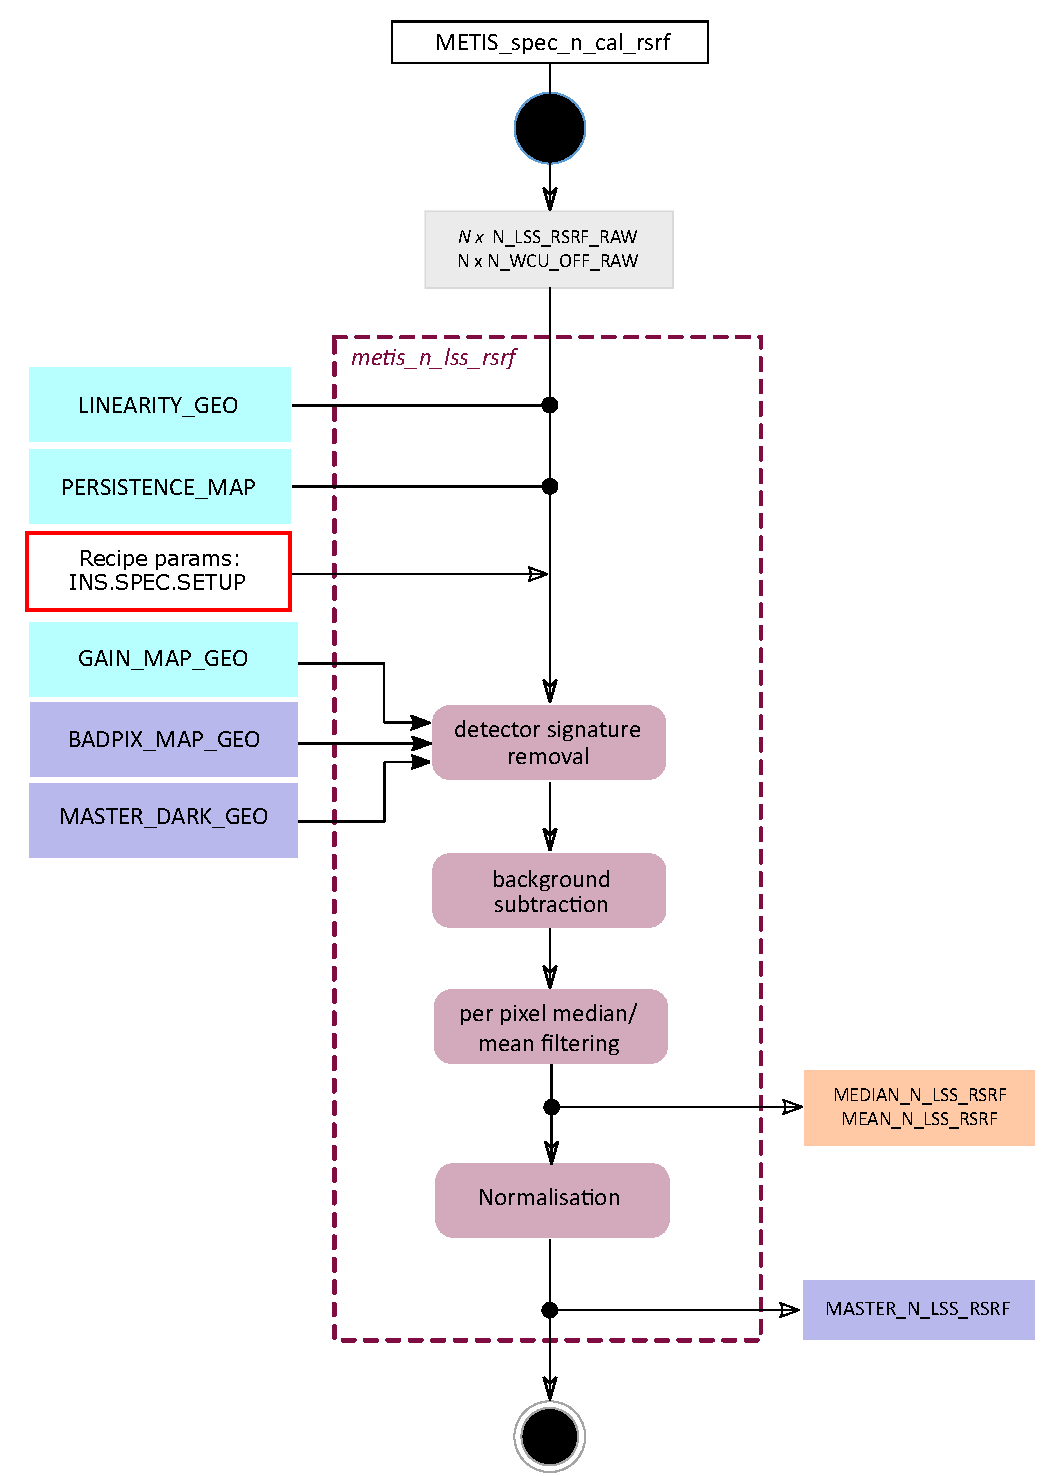
\includegraphics[width=0.5\textheight]{figures/metis_n_lss_rsrf_v0.84.pdf}
  \caption[Recipe: \REC*{metis_N_lss_rsrf}]{\REC*{metis_N_lss_rsrf} --
    Spectroscopic faltfielding with \ac{RSRF}.}
  \label{Fig:rec_n_lss_rsrf}
\end{figure}

\begin{recipedef}
Name:		& \REC{metis_N_lss_rsrf} \\
Purpose:	& Spectroscopic flatfielding with \ac{RSRF} \\
Type:		& Calibration\\
Requirements: & METIS-6084, METIS-3291, METIS-9099 \\
Templates:           & \TPL{METIS_spec_n_cal_rsrf} \\
Input data:     & $N\times$ \RAW{N_LSS_RSRF_RAW} \\
                & $N\times$ \RAW{N_WCU_OFF_RAW} \\
                & \EXTCALIB{PERSISTENCE_MAP}  \\
                & \STATCALIB{LINEARITY_GEO}  \\
                & \STATCALIB{GAIN_MAP_GEO}  \\
                & \EXTCALIB{BADPIX_MAP_GEO}   \\
                & \PROD{MASTER_DARK_GEO}  \\
Matched Keywords & \FITS{DET.DIT} \\
                 & \FITS{DET.NDIT}\\
                 & \FITS{DRS.SLIT}\\
Parameters: 	& exposure time\\
Algorithm:      & subtract master \ac{WCU} "OFF" frame from illumination frame (done on individual images)\\
                & median/mean filtering of subtracted images\\
                & division by blackbody spectrum\\
                & normalisation to achieve \ac{RSRF}\\
Output data:	&  \PROD{MASTER_N_LSS_RSRF} (\FITS{PRO.CATG}=\CODE{MASTER_N_LSS_TRSRF}): master flatfield/\ac{RSRF} \\
                & \PROD{MEDIAN_N_LSS_RSRF_IMG}: median map (\ac{QC})\\
                & \PROD{MEAN_N_LSS_RSRF_IMG}: mean map (\ac{QC})\\

Expected accuracies: & 3\% (cf.~\cite{METIS-calibration_plan} and~\cite{METIS_calerrbudget})\\
QC1 parameters: & \QC{QC N LSS RSRF MEAN LEVEL}: Mean level of the \ac{RSRF}\\
                & \QC{QC N LSS RSRF MEDIAN LEVEL}: Median level of the \ac{RSRF}\\
                & \QC{QC N LSS RSRF INTORDR LEVEL}: Flux level of the interorder background\\
                & \QC{QC N LSS RSRF NORM STDEV}: Standard deviation of the normalised \ac{RSRF}\\
                & \QC{QC N LSS RSRF NORM SNR}: \ac{SNR} of the normalised \ac{RSRF}\\
%                & more TBD\\
\end{recipedef}
%------------------------------------------------------------------------------------------------------------------
\clearpage
\subsubsection{\REC*{metis_N_lss_trace}:  Order detection}\label{rec:metis_n_lss_trace}
The recipe \REC{metis_N_lss_trace} aims at detecting the order and a polynomial fitting of the order location (see~\cite{pis02} and~\cite{pis21} for details on the algorithms). The detection and polynomial fitting is based on flatfield frames taken through a pinhole mask, which leads to individual pinhole traces along the entire dispersion direction.

\begin{figure}[ht]
  \centering
  \includegraphics[width=0.5\textheight]{figures/metis_N_lss_trace_v0.84.pdf}
  \caption[Recipe: \REC*{metis_N_lss_trace}]{\REC*{metis_N_lss_trace} --
    Detection and polynomial fitting of the order location.}
  \label{Fig:rec_N_lss_wave}
\end{figure}

\begin{recipedef}
Name:		& \REC{metis_N_lss_trace} \\
Purpose:	& Detection of order location \\
Type:		& Calibration\\
Requirements: & None \\
Templates:           & \TPL{METIS_spec_n_cal_rsrfpinh} \\
Input data:     & $N\times$ \RAW{N_LSS_RSRF_PINH_RAW} \\
                $N\times$ \RAW{N_WCU_OFF_RAW} \\
                & \EXTCALIB{PERSISTENCE_MAP}  \\
                & \STATCALIB{LINEARITY_GEO}  \\
                & \STATCALIB{GAIN_MAP_GEO}  \\
                & \EXTCALIB{BADPIX_MAP_GEO}   \\
                & \PROD{MASTER_DARK_GEO}  \\
                &  \PROD{MASTER_N_LSS_RSRF} \\
Matched Keywords & \FITS{DET.DIT} \\
                 & \FITS{DET.NDIT}\\
                 & \FITS{DRS.SLIT}\\
Parameters: 	& exposure time\\
Algorithm:      & Detection of the order edges\\
                & Polynomial fitting\\
Output data:	& \PROD{N_LSS_TRACE} (\FITS{PRO.CATG}=\CODE{N_LSS_TRACE}): Polynomial coefficients\\
Expected accuracies: & 1/10th of a pixel after post-processing\\
               & (cf.~\cite{METIS-calibration_plan}, R-MET-106, METIS-167, METIS-1371)\\
QC1 parameters: & \QC{QC N LSS TRACE LPOLYDEG}: Degree of the polynomial fit of the left order edge\\
                & \QC{QC N LSS TRACE LCOEFF<i>}: $i$-th coefficient of the polynomial of the left order edge\\
                & \QC{QC N LSS TRACE RPOLYDEG}: Degree of the polynomial fit of the right order edge\\
                & \QC{QC N LSS TRACE RCOEFF<i>}: $i$-th coefficient of the polynomial of the right order edge\\
                & \QC{QC N LSS TRACE INTORDR LEVEL}: Flux level of the interorder background\\
%                & \QC{TBD}: TBD\\
\end{recipedef}

\clearpage

%------------------------------------------------------------------------------------------------------------------
\subsubsection{\REC*{metis_N_lss_std}:  Standard star processing}\label{rec:metis_n_lss_std}
This recipe aims at processing standard stars used for the absolute flux calibration and (optionally) for the telluric feature removal: As first step the detector master calibration files derived previously are applied followed by the background subtraction, if needed the distortion correction (\PROD{N_LSS_DIST_SOL}), and
the wavelength calibration by means of the first guess solution (\PROD{N_LSS_WAVE_GUESS}) and the telluric sky lines (c.f. Sect.\,8.5 in~\cite{DRLS}). Then the recipe removes sky background, extracts the standard star spectrum object and collapses the 2D to 1D spectra. In case the \ac{STD} is used only for the flux calibration, a telluric correction is required to better compare the corresponding model spectrum. This is done by means of the standard star observations itself or (optionally) with a synthetic transmission curve (either a standard curve derived by the ESO Skycalc Tool\footnote{\url{https://www.eso.org/observing/etc/bin/gen/form?INS.MODE=swspectr+INS.NAME=SKYCALC}}, a standard curve (\STATCALIB{N_SYNTH_TRANS}) or \texttt{molecfit}. It is on the user's decision whether the standard star is used for the absolute flux calibration only, or also used for the telluric correction of the science target. The response function is then calculated as ratio of the measured 1d-\ac{STD} spectrum and a detailed model containing absolute flux information.

Please note that the procedure of the \ac{STD} handling changes when the classical method for the telluric correction is chosen. The reason is that in the response function, also the telluric features of the \ac{STD} star have to be present to be able to apply a combination of the telluric absorption removal and the conversion towards physical flux units (cf. Section~\ref{ssec:tellcorr}). In the case of using \texttt{molecfit}, a telluric correction is applied to the \ac{STD} spectrum to better determine the response function and only the response is delivered to the science recipes. In case of the classical approach with a \ac{STD}, the response function will also contain the telluric features of the \ac{STD}, and therefore a telluric correction beforehand is counterproductive.\\

\begin{figure}[ht]
  \centering
  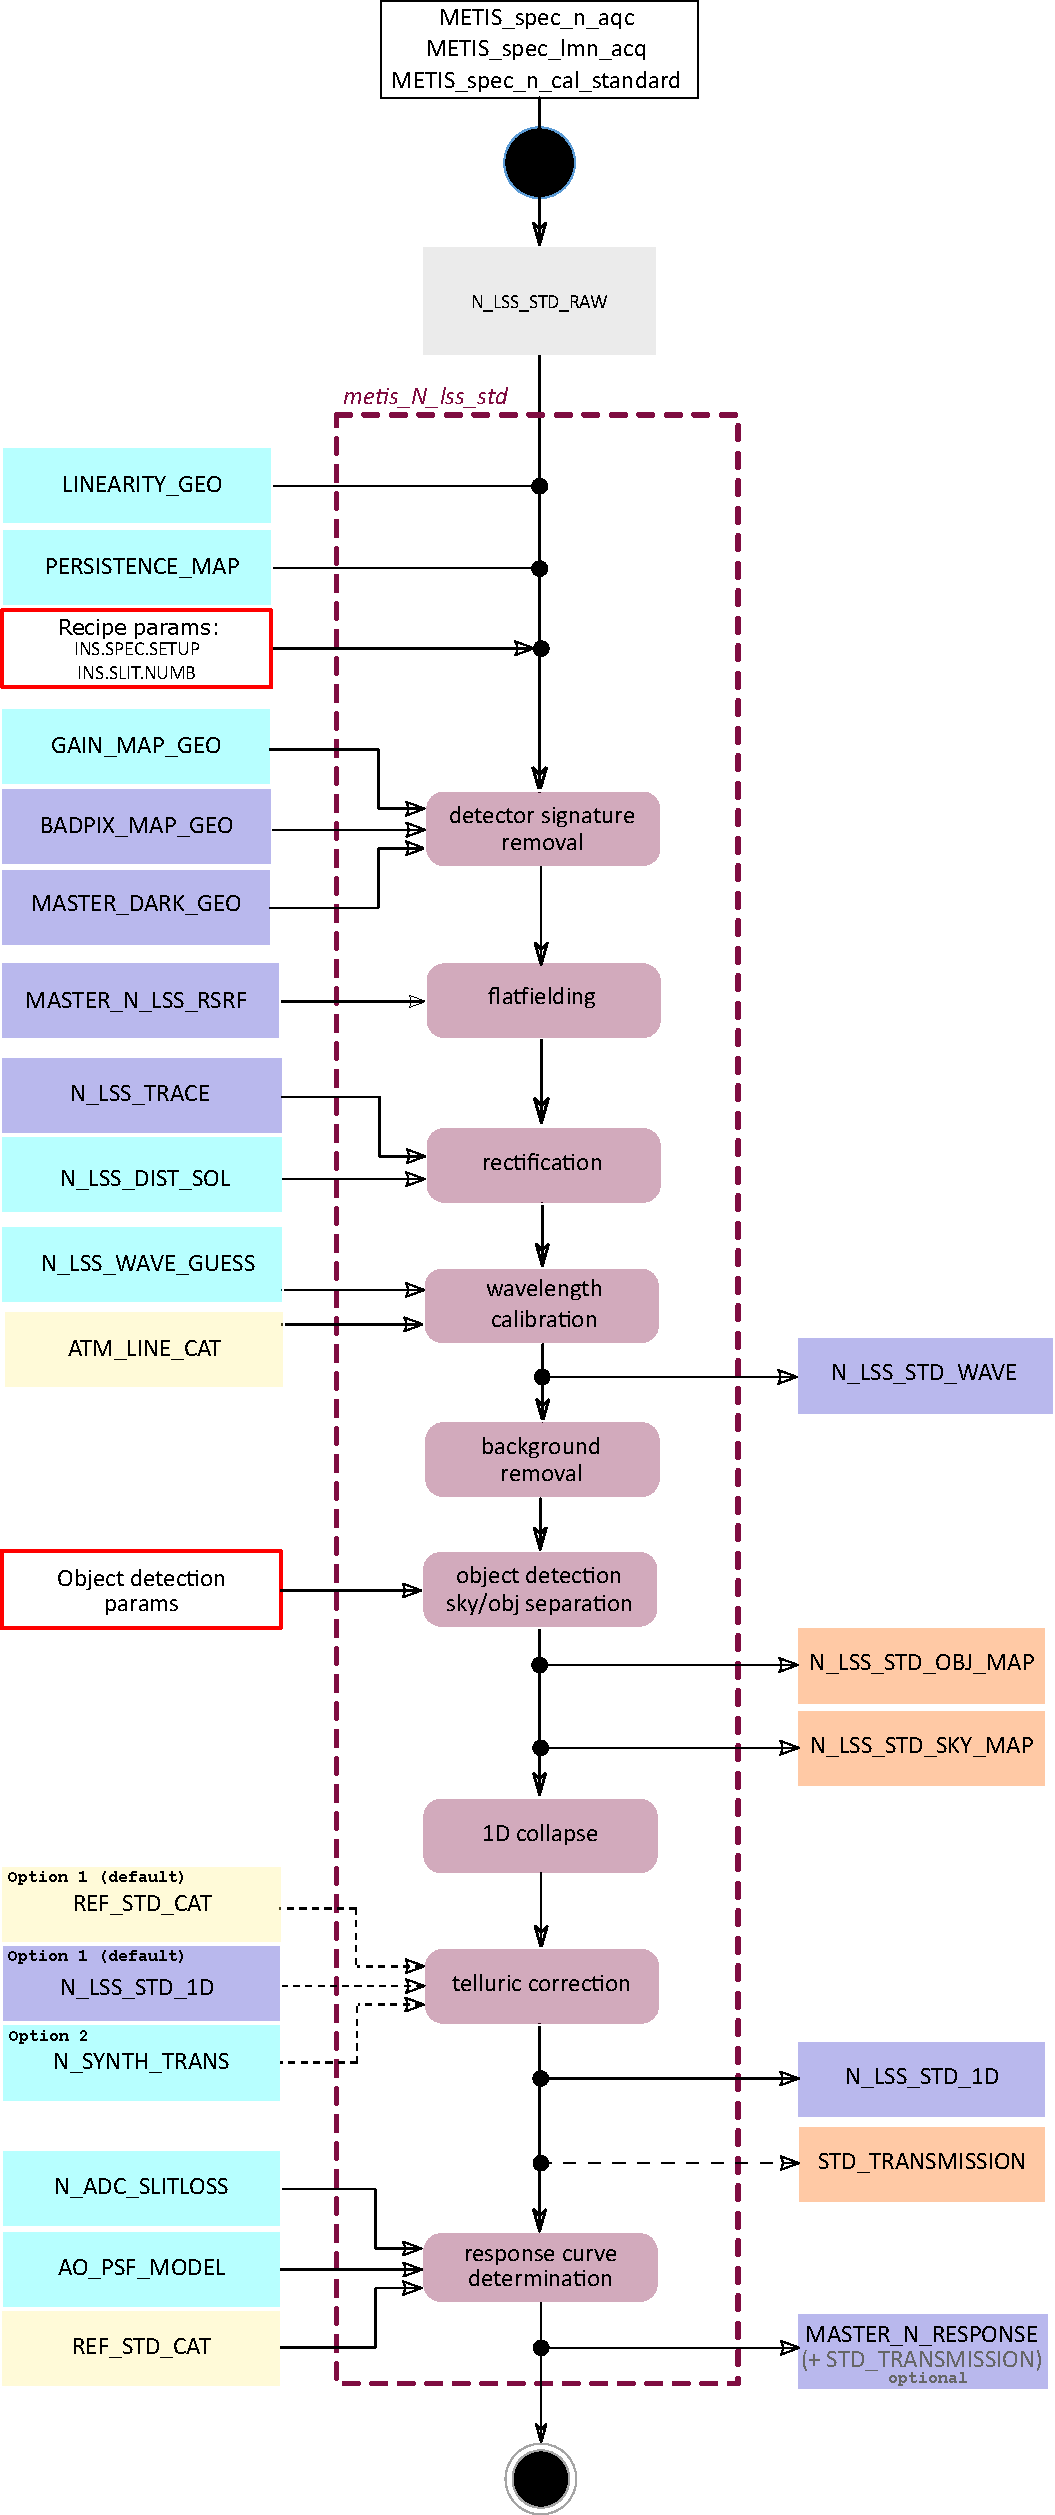
\includegraphics[width=0.4\textheight]{figures/metis_n_lss_std_v0.83.pdf}
  \caption[Recipe: \REC*{metis_N_lss_std}]{\REC*{metis_N_lss_std} --
    Standard star calibration recipe.}
  \label{Fig:rec_N_lss_flux}
\end{figure}
\clearpage
\begin{recipedef}
Name:		& \REC{metis_N_lss_std} \\
Purpose:	& Flux calibration \\
Type:		& Calibration\\
Requirements: & METIS-6084, METIS-6074, METIS-2757 \\
Templates:      & \TPL{METIS_spec_n_acq}, \\
                & \TPL{METIS_spec_lmn_acq}, \\
                & \TPL{METIS_spec_N_cal_standard}\\
                & \TPL{METIS_spec_lmn_obs_AutoChopNodOnSlit}\\
Input data: 	& \RAW{N_LSS_STD_RAW}\\
                & \EXTCALIB{PERSISTENCE_MAP}  \\
                & \STATCALIB{LINEARITY_GEO}  \\
                & \STATCALIB{GAIN_MAP_GEO}  \\
                & \EXTCALIB{BADPIX_MAP_GEO}   \\
                & \PROD{MASTER_DARK_GEO}  \\
                & \PROD{MASTER_N_LSS_RSRF} \\
                & \PROD{N_LSS_TRACE}\\
                & \STATCALIB{N_LSS_DIST_SOL} \\
                & \STATCALIB{N_LSS_WAVE_GUESS} \\
                & \STATCALIB{N_SYNTH_TRANS}\\
                & \EXTCALIB{AO_PSF_MODEL} \\
                & \EXTCALIB{ATM_LINE_CAT} \\
                & \STATCALIB{N_ADC_SLITLOSS}\\
                & \STATCALIB{REF_STD_CAT} \\                
Matched Keywords & \FITS{DET.DIT} \\
                 & \FITS{DET.NDIT}\\
                 & \FITS{DRS.SLIT}\\
Parameters: 	& exposure time, target information, nodding(/chopping parameters\\
Algorithm:      & Application of master calibration files\\
                & Determination and application of the wavelength solution\\
                & Background removal\\
                & Determination and application of the distortion correction\\
                & Identifying/separatiing sky/object pixels\\
                & Removing telluric lines\\
                & Collapsing 2D to 1D spectrum, (see Fig.\,\ref{Fig:rec_N_lss_sci})\\
                & Determination and application of response curve\\
Output data:	& \PROD{N_LSS_STD_OBJ_MAP}: Pixel map of object pixels (\ac{QC})\\
            	& \PROD{N_LSS_STD_SKY_MAP}: Pixel map of sky pixels (\ac{QC})\\
              	& \PROD{N_LSS_STD_1D}  : coadded, wavelength calibrated, collapsed 1D spectrum\\
                & \PROD{STD_TRANSMISSION}: Transmission curve derived by menas of the \ac{STD} star (\ac{QC})\\
                & \PROD{MASTER_N_RESPONSE}: response function (optionally including the transmission)\\
Expected accuracies: & for wavelength: 1/10th of a pixel after post-processing\\
            & (cf.~\cite{METIS-calibration_plan}, R-MET-106, METIS-167, METIS-1371)\\
            & for flux: 10\% over an atmospheric band \\
            & $<30$\% absolute line flux accuracy\\
            & $<5$\% absolute flux calibration \\
            & (cf.~\cite{METIS-calibration_plan}, R-MET-107, R-MET-82)\\
QC1 parameters: & \QC{QC N LSS STD BACKGD MEAN}: Mean value of background\\
                & \QC{QC N LSS STD BACKGD MEDIAN}: Median value of background\\
                & \QC{QC N LSS STD BACKGD STDEV}: Standard deviation value of background\\
                & \QC{QC N LSS STD SNR}: Signal-to-noise ration of flux standard star spectrum\\
                & \QC{QC N LSS STD NOISELEV}: Noise level of flux standard star spectrum\\
                & \QC{QC N LSS STD FWHM}: FWHM of flux standard spectrum\\
                & \QC{QC N LSS STD INTORDR LEVEL}: Flux level of the interorder background\\
                & \QC{QC N LSS STD AVGLEVEL}: Average level of the standard star flux \\
                & \QC{QC N LSS STD WAVECAL DEVMEAN}: Mean deviation from the
                  wavelength reference frame\\
                & \QC{QC N LSS STD WAVECAL FWHM}: Measured FWHM of lines\\
                & \QC{QC N LSS STD WAVECAL NIDENT}: Number of identified lines\\
                & \QC{QC N LSS STD WAVECAL NMATCH}: Number of lines matched between
                    catalogue and spectrum\\
                & \QC{QC N LSS STD WAVECAL POLYDEG}: Degree of the polynomial\\
                & \QC{QC N LSS STD WAVECAL POLYCOEFF<n>}: $n$-th coefficient of the polynomial\\
                & \QC{QC N LSS STD SNR}: Signal-to-noise ration of flux standard star spectrum\\
                & \QC{QC N LSS STD NOISELEV}: Noise level of flux standard star spectrum\\
                & \QC{QC N LSS STD FWHM}: FWHM of flux standard spectrum\\
%                & \QC{QC N LSS STD PSFLOSS}: Fraction of AO induced slit losses (TBdef)\\
%                & more TBD\\
\end{recipedef}

%------------------------------------------------------------------------------------------------------------------
\clearpage
\subsubsection{\REC*{metis_N_lss_sci}:  Science reduction}\label{rec:metis_n_lss_sci}
The science calibration recipe comprises the extraction of the object (i.e. separation of object/sky pixels), removing the sky lines, the application of the response curve previously defined. In case of a point/compact source, the 2D to 1D collapse is also done, otherwise 2D products are delivered. Finally, the spectra are coadded. The recipe also applies an absolute flux calibration (optionally with the telluric correction in one step, cf. Section~\ref{ssec:tellcorr}).
\begin{figure}[ht]
  \centering
  \includegraphics[width=0.35\textheight]{figures/metis_N_lss_sci_v0.83.pdf}
  \caption[Recipe: \REC*{metis_N_lss_sci}]{\REC*{metis_N_lss_sci} --
    Science reduction recipe.}
  \label{Fig:rec_N_lss_sci}
\end{figure}
\clearpage

\begin{recipedef}
Name:		& \REC{metis_N_lss_sci} \\
Purpose:  & Science data calibration\\
Type:		& Science reduction\\
Requirements: & METIS-6084 \\
Templates:      & \TPL{METIS_spec_n_acq}, \\
                & \TPL{METIS_spec_lmn_acq}, \\
                & \TPL{METIS_spec_n_obs_AutoChopNodOnSlit}, \\
                & \TPL{METIS_spec_lmn_obs_AutoChopNodOnSlit}\\
% HB 20230627 Template METIS_spec_N_obs_GenericOffset does not exist
%                 & \TPL{METIS_spec_N_obs_GenericOffset} \\
%                & \TPL{METIS_spec_n_cal_slit}\\
Input data: 	& \RAW{N_LSS_SCI_RAW}\\
                & \EXTCALIB{PERSISTENCE_MAP}  \\
                & \STATCALIB{LINEARITY_GEO}  \\
                & \STATCALIB{GAIN_MAP_GEO}  \\
                & \EXTCALIB{BADPIX_MAP_GEO}   \\
                & \PROD{MASTER_DARK_GEO}  \\
                & \PROD{MASTER_N_LSS_RSRF} \\
                & \PROD{N_LSS_TRACE}\\
                & \STATCALIB{N_LSS_DIST_SOL}\\
                & \STATCALIB{N_LSS_WAVE_GUESS}\\
                & \EXTCALIB{ATM_LINE_CAT} \\
                %& \EXTCALIB{AO_PSF_MODEL} \\
                & \STATCALIB{N_ADC_SLITLOSS}\\
                & \PROD{MASTER_N_RESPONSE} \\
Matched Keywords & \FITS{DET.DIT} \\
                 & \FITS{DET.NDIT}\\
                 & \FITS{DRS.SLIT}\\
Parameters: 	& exposure time, target information, nodding(/chopping parameters\\
Algorithm:      & Application of the detector master calib files\\
                & wavelength calibration \\
                & Identifying/separatiing sky/object pixels\\
                & Removing sky lines: Creation and Subtraction of 2D sky\\
                & Coaddition of individual object spectra of one OB\\
                & Collapsing 2D to 1D spectrum, (see Fig.\,\ref{Fig:rec_N_lss_sci})\\
                & Application of the response function (flux calibration) \\
Output data:	& \PROD{N_LSS_SCI_OBJ_MAP}: Pixel map of object pixels (\ac{QC})\\
            	& \PROD{N_LSS_SCI_SKY_MAP}: Pixel map of sky pixels (\ac{QC})\\
            	& \PROD{N_LSS_SCI_2D}: coadded, wavelength calibrated 2D spectrum\\
                & (\FITS{PRO.CATG}: \CODE{N_LSS_2d_coadd_wavecal}) \\
                & \PROD{N_LSS_SCI_1D}: coadded, wavelength calibrated 1D spectrum\\
                & (\FITS{PRO.CATG}: \CODE{N_LSS_1d_coadd_wavecal}) \\
                & \PROD{N_LSS_SCI_FLUX_2D}: coadded, wavelength calibrated 2D spectrum\\
                & (\FITS{PRO.CATG}: \CODE{N_LSS_2d_coadd_wavecal}) \\
              	& \PROD{N_LSS_SCI_FLUX_1D}: coadded, wavelength 1D spectrum\\
                & (\FITS{PRO.CATG}: \CODE{N_LSS_1d_coadd_wavecal}) \\
Expected accuracies: & for wavelength: 1/10th of a pixel after post-processing\\
            & (cf.~\cite{METIS-calibration_plan}, R-MET-106, METIS-167, METIS-1371)\\
            & for flux: 10\% over an atmospheric band \\
            & $<30$\% absolute line flux accuracy\\
            & $<5$\% absolute flux calibration \\
            & (cf.~\cite{METIS-calibration_plan}, R-MET-107, R-MET-82)\\
            & for optional telluric correction: 10\% within an atmospheric band); desired: 2\% 
            (\cite{METIS-calibration_plan})\\
QC1 parameters: & \QC{QC N LSS SCI SNR}: Signal-to-noise ration of science spectrum\\
                & \QC{QC N LSS SCI NOISELEV}: Noise level of science spectrum\\
                & \QC{QC N LSS SCI FLUX SNR}: Signal-to-noise ration of flux calibrated  science spectrum\\
                & \QC{QC N LSS SCI FLUX NOISELEV}: Noise level of flux calibrated science spectrum\\
                & \QC{QC N LSS SCI INTORDR LEVEL}: Flux level of the interorder background\\
                & \QC{QC N LSS SCI WAVECAL DEVMEAN}: Mean deviation from the wavelength reference frame\\
                & \QC{QC N LSS SCI WAVECAL FWHM}: Measured FWHM of lines\\
                & \QC{QC N LSS SCI WAVECAL NIDENT}: Number of identified lines\\
                & \QC{QC N LSS SCI WAVECAL NMATCH}: Number of lines matched between catalogue and spectrum\\
                & \QC{QC N LSS SCI WAVECAL POLYDEG}: Degree of the wavelength polynomial\\
                & \QC{QC N LSS SCI WAVECAL POLYCOEFF<n>}: $n$-th coefficient of the polynomial\\
%                & more TBD\\
\end{recipedef}

%------------------------------------------------------------------------------------------------------------------
\clearpage
\subsubsection{\REC*{metis_N_lss_mf_model}:  Telluric correction}\label{rec:metis_n_lss_mf_model}
The telluric correction will be done with the package \texttt{molecfit}\footnote{\url{https://www.eso.org/sci/software/pipelines/molecfit/molecfit-pipe-recipes.html}}. It is realised in three individual recipes, \REC{metis_N_lss_mf_model}, which calculates the best-fit model, \REC{metis_N_lss_mf_calctrans}, which creates a synthetic transmission curve, and \REC{metis_N_lss_mf_correct}, which performs the actual telluric correction by means of the synthetic transmission.

\begin{figure}[ht]
  \centering
  \includegraphics[width=0.5\textheight]{figures/metis_N_lss_mf_model_v0.83.pdf}
  \caption[Recipe: \REC*{metis_N_lss_mf_model}]{\REC*{metis_N_lss_mf_model} --
    Recipe to achieve the best-fit for the calculation of the synthetic transmission curve for the telluric correction.}
  \label{Fig:rec_N_lss_mf_model}
\end{figure}
\clearpage

\begin{recipedef}
Name:		& \REC{metis_N_lss_mf_model}\\
Purpose:	& Achieve the best fit for modelling the transmission curve to be applied as telluric correction \\
Type:		& Post-calibration\\
Requirements: & METIS-4051, METIS-6091 \\
Templates:           & None\\
Input data: 	& \PROD{N_LSS_SCI_FLUX_1D}\\
                & \STATCALIB{LSF_KERNEL} \\
                & \EXTCALIB{ATM_PROFILE} \\
                & \EXTCALIB{ATM_LINE_CAT} \\
Matched Keywords & \FITS{DRS.SLIT}\\
Parameters: 	& \texttt{molecfit} parameters (c.f. \cite{molecfit})\\
Algorithm:      & Fit of telluric features visible in the science input spectrum\\
                & Determination of best-fit parameter set\\
Output data:	& \PROD{MF_BEST_FIT_TAB}\\
Expected accuracies: & n/a\\
QC1 parameters: & cf.~\cite{molecfit}\\
\end{recipedef}

%------------------------------------------------------------------------------------------------------------------
\clearpage
\subsubsection{\REC*{metis_N_lss_mf_calctrans}:  Telluric correction}\label{rec:metis_n_lss_mf_calctrans}
\begin{figure}[ht]
  \centering
  \includegraphics[width=0.5\textheight]{figures/metis_N_lss_mf_calctrans_v0.83.pdf}
  \caption[Recipe: \REC*{metis_N_lss_mf_calctrans}]{\REC*{metis_N_lss_mf_calctrans} --
    Recipe to calculate the synthetic transmission to be applied as telluric correction.}
  \label{Fig:rec_N_lss_mf_calctrans}
\end{figure}
\clearpage

\begin{recipedef}
Name:		& \REC{metis_N_lss_mf_calctrans}\\
Purpose:	& Calculation of the synthetic transmission \\
Type:		& Post-calibration\\
Requirements: & METIS-4051, METIS-6091 \\
Templates:           & None\\
Input data: 	& \PROD{MF_BEST_FIT_TAB}\\
                & \STATCALIB{LSF_KERNEL} \\
                & \EXTCALIB{ATM_PROFILE} \\
                & \EXTCALIB{ATM_LINE_CAT} \\
Matched Keywords & \FITS{DRS.SLIT}\\
Parameters: 	& \texttt{molecfit} parameters (c.f.  \cite{molecfit})\\
Algorithm:      & Calculate the entire transmission curve by means of the best-fit parameters\\
Output data:	& \PROD{N_LSS_SYNTH_TRANS}\\
\\
Expected accuracies: & n/a\\
QC1 parameters: & cf.~\cite{molecfit}\\
\end{recipedef}

%------------------------------------------------------------------------------------------------------------------
\clearpage
\subsubsection{\REC*{metis_N_lss_mf_correct}:  Telluric correction}\label{rec:metis_n_lss_mf_correct}
\begin{figure}[ht]
  \centering
  \includegraphics[width=0.5\textheight]{figures/metis_N_lss_mf_correct_v0.83.pdf}
  \caption[Recipe: \REC*{metis_N_lss_mf_correct}]{\REC*{metis_N_lss_mf_correct} --
    Recipe to apply the telluric correction.}
  \label{Fig:rec_N_lss_mf_correct}
\end{figure}
\clearpage

\begin{recipedef}
Name:		& \REC{metis_N_lss_mf_correct}\\
Purpose:	& Apply the synthetic transmission to the science spectra \\
Type:		& Post-calibration\\
Requirements: & METIS-4051, METIS-6091 \\
Templates:           & None\\
Input data: 	& \PROD{N_LSS_SCI_FLUX_1D}\\
                & \PROD{N_LSS_SYNTH_TRANS}\\
Matched Keywords & \FITS{DRS.SLIT}\\
Parameters: 	& None\\
Algorithm:      & Apply telluric correction, i.e. divide the input science spectrum\\
                & by the synthetic transmission\\
Output data:	& \PROD{N_LSS_SCI_FLUX_TELLCORR_1D}\\
Expected accuracies: & Telluric removal must be good enough to reach the required spectro-photometric accuracy (10\% within an atmospheric band). Desired: 2\% (\cite{METIS-calibration_plan})\\
QC1 parameters: & cf.~\cite{molecfit}\\
\end{recipedef}








%% 06_5-Recipes_IFU.tex
%% Created:     Fri Aug 25 13:14:02 2017 by Koehler@I-Mac
%%
%% subsection for IFU recipes
%%
%%%%%%%%%%%%%%%%%%%%%%%%%%%%%%%%%%%%%%%%%%%%%%%%%%%%%%%%%%%%%%%%%%%%%%%%%%%%%%%

\clearpage
\subsection{LM integral-field spectroscopy (IFU)}
\label{ssec:IFU_recipes}

\TODO{This section is identical to the PDR document \cite{DRLS}. We
will consider rearranging the recipes to be in line with the imaging
pipelines. This would entail handling basic reduction and background
subtraction for both science and standard exposures in common
recipes (\CODE{metis_ifu_basic}, \CODE{metis_ifu_background}), then
having a recipe to analyse the standard observations
(\CODE{metis_ifu_photstd}). The science exposures are then fully
calibrated (\REC{metis_ifu_calibrate}). A full set of exposures would
then be assembled and restored with a fully sampled PSF in a
post-processing recipe (\CODE{metis_ifu_combine}).}

\subsubsection{IFU wavelength calibration}
\label{sssec:ifu_wavecal}
\label{rec:metis_ifu_wavecal}

This recipe processes daytime wavelength calibration images to derive
the pixel-to-wavelength relation for the LM integral-field
spectrograph. The calibration template will use the \ac{QCL} in the warm calibration unit to finely sample the desired
wavelength range. The image will consist of lines for each wavelength
and slice. The solution will have to provide for each detector pixel
$(x,y)$ the slice number $i$, the spatial position $\xi$ along the
slice and the wavelength in the dispersion correction. As the slices
and wavelength lines may be tilted with respect to the detector
columns and rows, a combined solution is required
\begin{eqnarray}
  \label{eq:wavelength_solution}
  \xi &= f_{i}(x, y) \\
  \lambda &= g_{i}(x, y)
\end{eqnarray}
The boundaries of the slice image on the detector are obtained by
measuring the left and right edges of the wavelength lines and
interpolating. The slice number is then obtained by counting the
slices according to the optical design of the spectrograph. The
wavelength of each line is known from the settings of the \ac{QCL}, the $x$
coordinate is obtained by linear interpolation along the line (or
perhaps using the distortion table from \hyperref[rec:metis_ifu_distortion]{\REC{metis_ifu_distortion}} if
necessary). The functions $f_{i}$ and $g_{i}$ are expected to be
sufficiently accurately described by low-order polynomials.

The recipe produces a multi-extension FITS file with an image
extension mapping wavelength across each detector in the array. A
table extension holds the polynomial coefficients.

 This is in compliance with \REQ{METIS-6074}.

\begin{recipedef}
  Name:                & \hyperref[rec:metis_ifu_wavecal]{\REC{metis_ifu_wavecal}}              \\
  Purpose:             & Determine pixel-to-wavelength transformation.                          \\
  Requirements:        & \REQ{METIS-6074}                                                       \\
  Type:                & Calibration                                                            \\
  Templates:           & \TPL{METIS_ifu_cal_InternalWave}                                       \\
  Input data:          & Images taken with WCU \ac{QCL} source                                  \\
                       & \hyperref[dataitem:master_dark_ifu]{\PROD{MASTER_DARK_IFU}}            \\
                       & Bad-pixel map                                                          \\
                       & Distortion table (TBD)                                                 \\
  Parameters:          & TBD                                                                    \\
  Algorithm:           & Measure line locations (left and right edges, centroid by Gaussian fit)\\
                       & Compute wavelength solution $\xi(x, y, i)$, $\lambda(x, y, i)$         \\
  Output data:         & \hyperref[dataitem:ifu_wavecal]{\PROD{IFU_WAVECAL}}                    \\
  Expected accuracies: & TBD                                                                    \\
  QC1 parameters:      & \QC{QC IFU WAVECAL RMS}                                                \\
                       & \QC{QC IFU WAVECAL NLINES}                                             \\
                       & \QC{QC IFU WAVECAL PEAK CNTS}                                          \\
                       & \QC{QC IFU WAVECAL LINE WIDTH}                                         \\
  \end{recipedef}

\begin{figure}[hb]
  \centering
  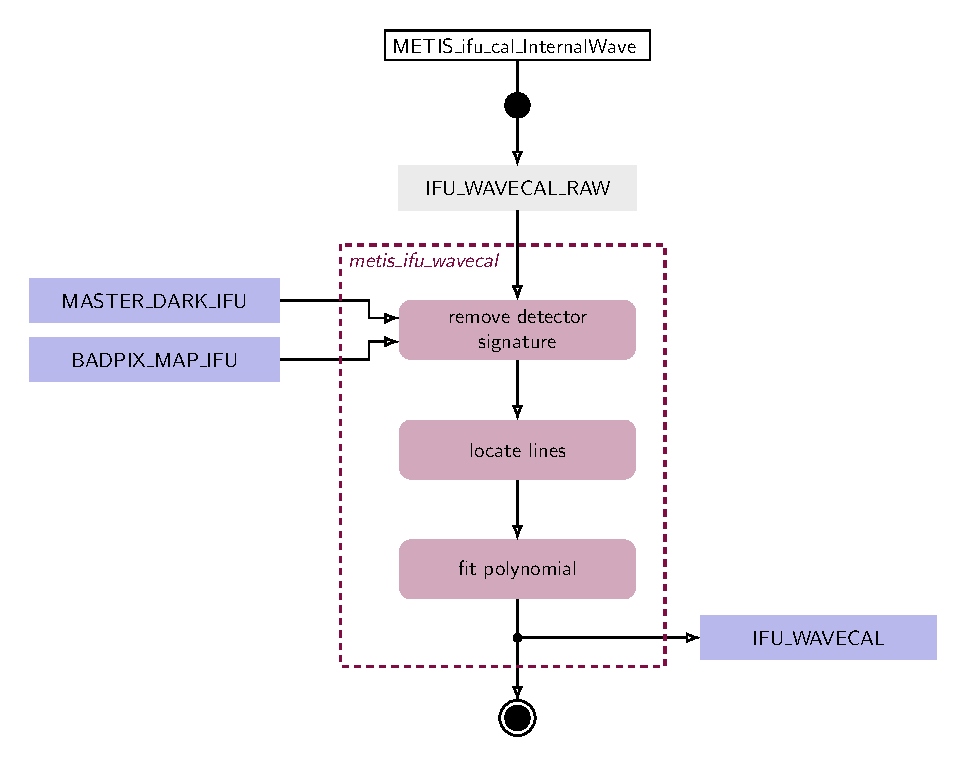
\includegraphics[width=0.7\textwidth]{metis_ifu_wavecal}
  \caption[Recipe: \REC{metis_ifu_wavecal}]{\REC{metis_ifu_wavecal} --
    daytime wavelength calibration for the IFU.}
  \label{fig:metis_ifu_wavecal}
\end{figure}


\clearpage
\subsubsection{IFU relative spectral response function}
\label{sssec:ifu_rsrf}
\label{rec:metis_ifu_rsrf}

This recipe creates a spectroscopic master flat and determines the
relative spectral response function (RSRF) for the four HAWAII2RG
detectors of the LM spectrograph. The input data are obtained by
illuminating the field of view with the black-body calibration lamp at
two different temperatures. The RSRF is then determined by dividing
the image by the known lamp continuum shape for the respective
temperature. We refer to the two-dimensional image obtained by this
division as \hyperref[dataitem:master_flat_ifu]{\PROD{MASTER_FLAT_IFU}} and the one-dimensional reponse
function obtained by averaging at constant wavelength as
\PROD{RSRF}. The bad pixel mask can be updated by identifying pixels
that deviate strongly from their neighbours.

\begin{recipedef}
Name:                & \hyperref[rec:metis_ifu_rsrf]{\REC{metis_ifu_rsrf}}                                                     \\
Purpose:             & Create relative spectral response function for the IFU detector.         \\
Requirements:        & \REQ{METIS-6131}, \REQ{METIS-6698}                                       \\
Type:                & Calibration                                                              \\
Templates:           & \TPL{METIS_ifu_cal_rsrf}                                                 \\
Input data:          & Raw flats taken with black-body calibration lamp.                        \\
                     & \hyperref[dataitem:master_dark_ifu]{\PROD{MASTER_DARK_IFU}}              \\
                     & \hyperref[dataitem:badpix_map_ifu]{\PROD{BADPIX_MAP_IFU}}                                                    \\
                     & \hyperref[dataitem:ifu_wavecal]{\PROD{IFU_WAVECAL}}: image with wavelength at each pixel.                 \\
Parameters:          & TBD                                                                      \\
Algorithm:           & Create continuum image by mapping Planck spectrum at $T_{\mathrm{lamp}}$ to
                       wavelength image.                                                        \\
                     & Divide exposures by continuum image.                                     \\
                     & Average exposures to yield master flat (2D RSRF).                        \\
                     & Average in spatial direction to obtain relative response function        \\
Output data:         & \hyperref[dataitem:master_flat_ifu]{\PROD{MASTER_FLAT_IFU}}                                                   \\
                     & \hyperref[dataitem:rsrf_ifu]{\PROD{RSRF_IFU}}                                                          \\
                     & \hyperref[dataitem:badpix_map_ifu]{\PROD{BADPIX_MAP_IFU}}                                                    \\
Expected accuracies: & TBD                                                                      \\
QC1 parameters:      & \QC{QC IFU RSRF NBADPIX}                                                    \\
                     & (more TBD)                                                               \\
\end{recipedef}

\begin{figure}[hb]
  \centering
  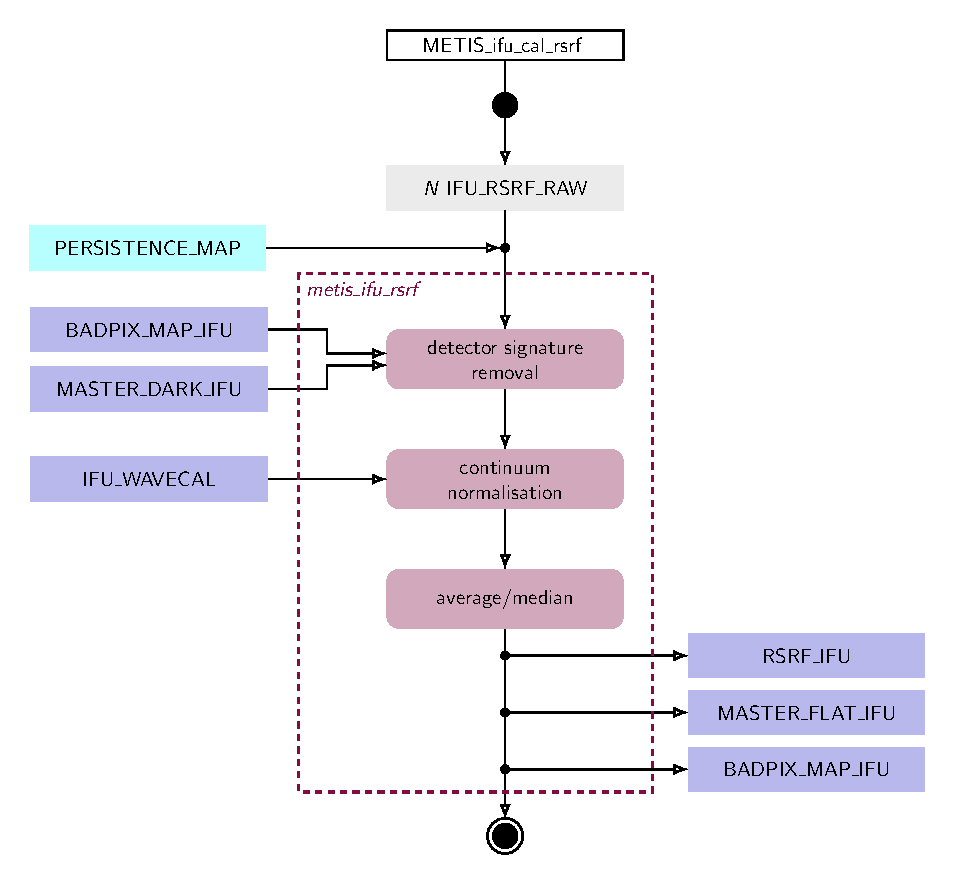
\includegraphics[width=0.6\textwidth]{metis_ifu_rsrf}
  \caption[Recipe: \REC{metis_ifu_rsrf}]{\REC{metis_ifu_rsrf} --
    creation of IFU relative spectral response function.}
  \label{fig:metis_ifu_rsrf}
\end{figure}


\clearpage
\subsubsection{IFU flux standard reduction}
\label{sssec:ifu_std_process}
\label{rec:metis_ifu_std_process}

This recipe reduces and analyses a series of IFU observations of a
spectroscopic flux standard star. The comparison of the measured
detector counts (ADU) with the tabulated spectrum of the star gives
the wavelength-dependent conversion from ADU to physical units
(photons per second per per centimetre square per wavelength bin per
spatial bin).

The level of stray light is estimated in the dark areas between the
spectra and subtracted from the entire frame. The distribution of
stray light across the field can only be characterised once the
instrument is built. It is to be hoped that subtraction of a constant
or a low-level 2D polynomial fit will be sufficient.

The sky and thermal background is estimated from blank sky
observations (if obtained during the observing sequence) or by
combining the (dithered) science frames.

The wavelength calibration is taken from the daylight calibration. It
may be refined by measuring telluric emission and/or absorption lines
(by fitting with \lstinline{molecfit}).

\begin{recipedef}
  Name:                & \hyperref[rec:metis_ifu_std_process]{\REC{metis_ifu_std_process}}                                            \\
  Purpose:             & Determine conversion between detector counts and physical source flux. \\
  Requirements:        & \REQ{METIS-6131}                                                       \\
  Type:                & Calibration                                                            \\
  Templates:           & \TPL{METIS_ifu_cal_standard}                                           \\
  Input data:          & Raw spectra of flux standard star                                      \\
                       & \hyperref[dataitem:master_dark_ifu]{\PROD{MASTER_DARK_IFU}}            \\
                       & Master flat (2D relative spectral response function)                   \\
                       & Bad pixel mask                                                         \\
                       & Wavelength calibration image                                           \\
                       & Distortion table                                                       \\
  Parameters:          & TBD                                                                    \\
  Algorithm:           & Subtract dark, divide by master flat                                   \\
                       & Estimate stray light and subtract                                      \\
                       & Estimate background and subtract                                       \\
                       & Rectify spectra and assemble cube                                      \\
                       & Extract 1D spectrum of star                                            \\
                       & Compute and apply telluric correction                                  \\
                       & Compute conversion to physical units as function of wavelength.        \\
  Output data:         & \hyperref[dataitem:ifu_std_reduced_cube]{\PROD{IFU_STD_REDUCED_CUBE}}  \\
                       & \hyperref[dataitem:ifu_std_background_cube]{\PROD{IFU_STD_BACKGROUND_CUBE}}                                         \\
                       & \hyperref[dataitem:ifu_std_reduced_1d]{\PROD{IFU_STD_REDUCED_1D}}                                              \\
                       & \hyperref[dataitem:ifu_std_telluric_1d]{\PROD{IFU_STD_TELLURIC_1D}}                                             \\
                       & \hyperref[dataitem:fluxcal_tab]{\PROD{FLUXCAL_TAB}}                                                     \\
  Expected accuracies: & TBD                                                                    \\
  QC1 parameters:      & \QC{QC IFU STD STRAYLIGHT MEAN}                                        \\
\end{recipedef}

\begin{figure}[hb]
  \centering
  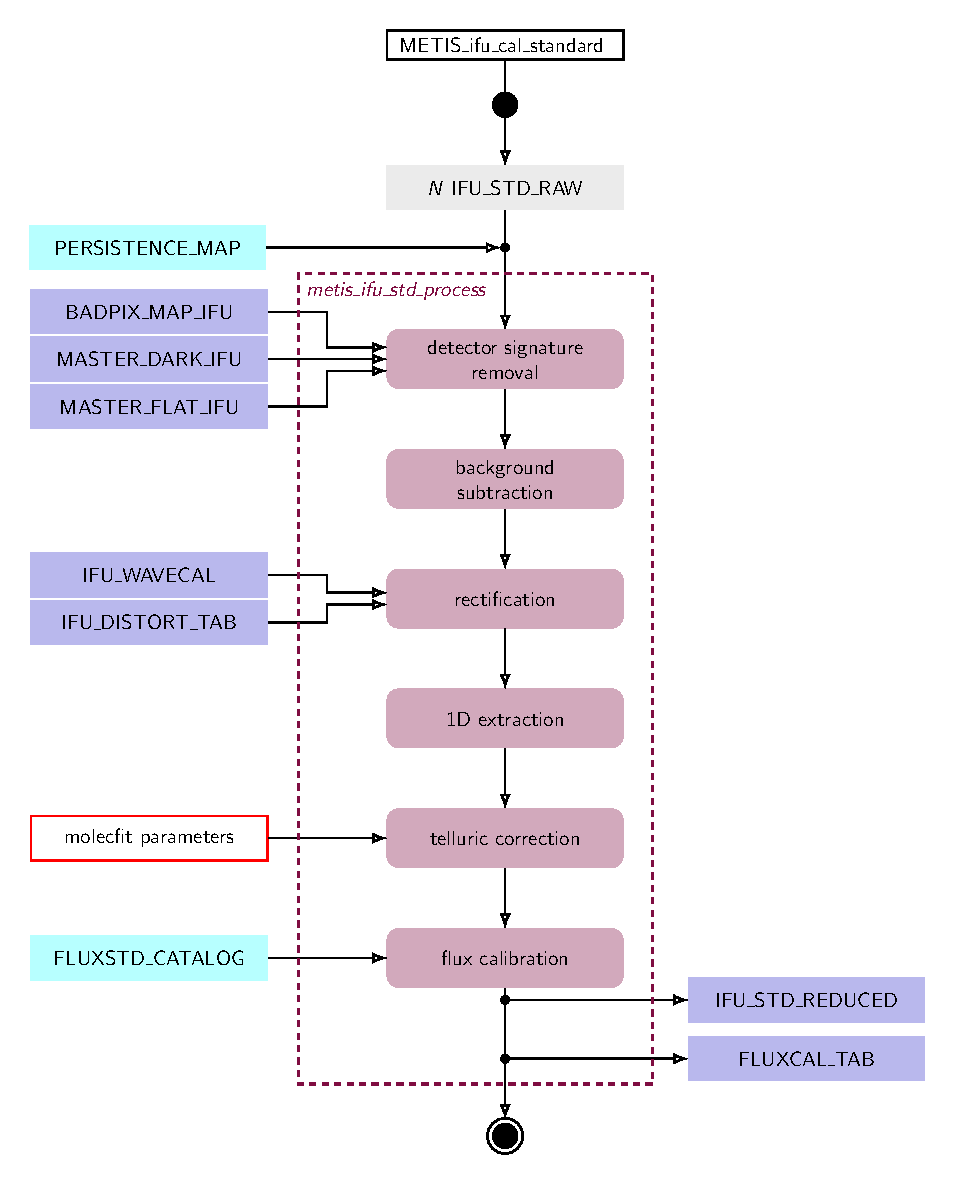
\includegraphics[width=0.7\textwidth]{metis_ifu_std_process}
  \caption[Recipe: \REC{metis_ifu_std_process}]{%
    \hyperref[rec:metis_ifu_std_process]{\REC{metis_ifu_std_process}} -- reduction of IFU flux standard
    frames and flux calibration (not all data products are shown).}
  \label{fig:metis_ifu_std_process}
\end{figure}

\clearpage
\subsubsection{IFU science reduction}
\label{sssec:ifu_sci_process}
\label{rec:metis_ifu_sci_process}

This recipe performs basic reduction of raw science exposures applying
dark and RSRF correction and flux calibration (i.e.~conversion of
pixel values to physical units) on each exposure individually. The
recipe shall be able to process data from either the nominal or the
extended wavelength mode. For the nominal mode, all slices belong to
the same echelle order. For the extended mode, slices belonging to the
same echelle order are grouped and processing is iterated over the
echelle orders.

The level of stray light is estimated in the dark areas between the
spectra and subtracted from the entire frame. The distribution of
stray light across the field can only be characterised once the
instrument is built. It is to be hoped that subtraction of a constant
or a low-level 2D polynomial fit will be sufficient.

The sky and thermal background, as well as residual straylight, is
estimated from blank sky observations if these are available in the
sequence of input frames or by combining (dithered) science
frames. The initial wavelength solution is taken from the daylight
calibration. It may be checked and corrected by measuring atmospheric
lines if a sufficient number is available in the limited wavelength
range.

A telluric correction is determined by this recipe by automatically
extracting a 1D spectrum from ``object'' pixels identified by a
thresholding algorithm. \lstinline{molecfit} is applied to this
spectrum and the correction is mapped back to the reduced 2D images or
3D cubes using the wavelength images. In an interactive environment
(Reflex workflow) the telluric correction may be improved by asking
the user to define an extraction aperture adapted to the target
structure.

Various levels of output data can be envisaged:
\begin{itemize}
\item Reduced 2D detector images. These are accompanied by additional
  information describing the geometry of the slice layout, target
  position and wavelength calibration to the extent that the exposure can be
  combined with other exposures into a single rectified spectral cube.
  This information can be stored in the FITS header or a table
  extension.
\item A rectified spectral cube for each exposure with a linear
  wavelength grid, constructed by resampling each spectral slice onto
  a spatial-wavelength grid common to all slices. The spatial pixels
  are rectangular with along-slit pixel scale given by the detector
  pixel scale and the across-slit pixel scale given by the slice
  width.
\item A spectral cube obtained by combining all exposures taken within
  a template. This step involves the image reconstruction discussed in
  Sect.~8.9 of \cite{DRLS}. Whether this step is included
  in the present recipe \hyperref[rec:metis_ifu_sci_process]{\REC{metis_ifu_sci_process}} or is postponed to
  the more general recipe \hyperref[rec:metis_ifu_sci_postprocess]{\REC{metis_ifu_sci_postprocess}} is TBD. It
  may be formally required to do the image reconstruction here if
  templates are set up to obtain a fixed set of spatially dithered and
  rotated exposures aimed at reconstructing a fully sampled PSF in
  both spatial dimensions.
\end{itemize}

For the nominal mode, each output is a single-extension FITS file
corresponding to one echelle order. For the extended mode, each of the
echelle orders results in an extension in a multi-extension FITS
file.

The recipe as descibed here is run in the science pipelines. For the
observatory pipeline, a variant of the recipe may be implemented with
reduced functionality and output. The observatory recipe may also have
to include features to determine QC parameters for the LM-band images
that are taken in parallel with the IFU exposures, similar to
\REC{metis_lm_img_sci_process} (Sect.~\ref{ssec:recipes_img_lm}).

\begin{recipedef}
Name:                & \hyperref[rec:metis_ifu_sci_process]{\REC{metis_ifu_sci_process}}                                                              \\
Purpose:             & Reduction of individual science exposures.                                               \\
Requirements:        & \REQ{METIS-6131}                                                                         \\
Type:                & Science                                                                                  \\
Templates:           & \TPL{METIS_ifu_obs_FixedSkyOffset}                                                       \\
                     & \TPL{METIS_ifu_obs_GenericOffset}                                                        \\
                     & \TPL{METIS_ifu_ext_obs_FixedSkyOffset}                                                   \\
                     & \TPL{METIS_ifu_ext_obs_GenericOffset}                                                    \\
% TODO: Decide what to do about app
%                     & \TPL{METIS_ifu_app_obs_GenericOffset}                                                    \\
                     & \TPL{METIS_ifu_vc_obs_FixedSkyOffset}                                                    \\
%                     & \TPL{METIS_ifu_ext_app_obs_GenericOffset}                                                \\
                     & \TPL{METIS_ifu_ext_vc_obs_FixedSkyOffset}                                                \\
                     & \TPL{METIS_ifu_cal_psf}                                                                  \\
Input data:          & Dithered science exposures.                                                              \\
                     & Blank sky images (if available)                                                          \\
                     & \hyperref[dataitem:master_dark_ifu]{\PROD{MASTER_DARK_IFU}}                              \\
                     & Master flat (2D relative spectral response function)                                     \\
                     & Bad pixel mask                                                                           \\
                     & Wavelength calibration image                                                             \\
                     & Flux calibration table                                                                   \\
                     & Distortion table                                                                         \\
                     & Line spread kernel to be used with \CODE{molecfit}                                       \\
Parameters:          & telluric correction (yes/no)                                                             \\
                     & more TBD                                                                                 \\
Algorithm:           & Subtract dark, divide by master flat                                                     \\
                     & Estimate stray light and subtract                                                        \\
                     & Estimate background from dithered science exposures or blank-sky exposures and subtract. \\
                     & Apply flux calibration.                                                                  \\
                     & Rectify spectra and assemble cube                                                        \\
                     & Extract 1D object spectrum                                                               \\
                     & Compute telluric correction and apply to reduced images and cube                         \\
Output data:         & \hyperref[dataitem:ifu_sci_reduced]{\PROD{IFU_SCI_REDUCED}} (2D, per exposure)           \\
                     & \hyperref[dataitem:ifu_sci_reduced_tac]{\PROD{IFU_SCI_REDUCED_TAC}} (2D, per exposure)   \\
                     & \hyperref[dataitem:ifu_sci_background]{\PROD{IFU_SCI_BACKGROUND}} (2D, per exposure)     \\
                     & \hyperref[dataitem:ifu_sci_reduced_cube]{\PROD{IFU_SCI_REDUCED_CUBE}} (3D, per exposure) \\
                     & \hyperref[dataitem:ifu_sci_reduced_cube_tac]{\PROD{IFU_SCI_REDUCED_CUBE_TAC}} (3D, per exposure) \\
                     & \hyperref[dataitem:ifu_sci_combined]{\PROD{IFU_SCI_COMBINED}} (3D)                       \\
                     & \hyperref[dataitem:ifu_sci_combined_tac]{\PROD{IFU_SCI_COMBINED_TAC}} (3D)               \\
                     & \hyperref[dataitem:ifu_sci_object_1d]{\PROD{IFU_SCI_OBJECT_1D}}  (1D)                    \\
                     & \hyperref[dataitem:ifu_sci_telluric_1d]{\PROD{IFU_SCI_TELLURIC_1D}}                      \\
Expected accuracies: & TBD                                                                                      \\
QC1 parameters:      & TBD                                                                                      \\
\end{recipedef}

\begin{figure}[hb]
  \centering
  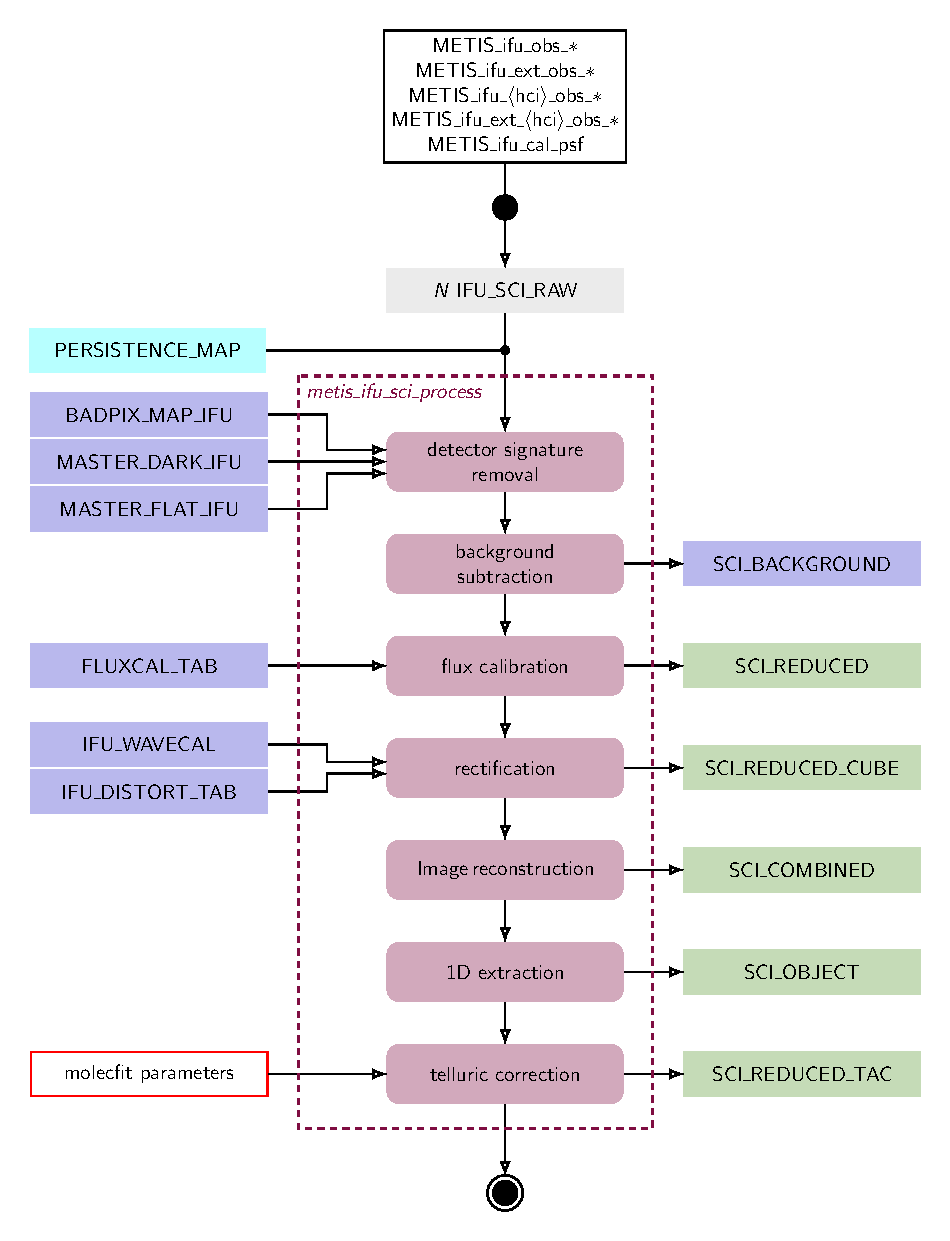
\includegraphics[width=0.7\textwidth]{metis_ifu_sci_process}
  \caption[Recipe: \REC{metis_ifu_sci_process}]{%
    \hyperref[rec:metis_ifu_sci_process]{\REC{metis_ifu_sci_process}} -- reduction of IFU science frames.}
  \label{fig:metis_ifu_sci_process}
\end{figure}



\clearpage
\subsubsection{IFU telluric absorption correction}
\label{sssec:ifu_tellcorr}
\label{rec:metis_ifu_tellcorr}

This recipe corrects for telluric absorption in a reduced IFU data
cube. The correction is done via a model atmospheric spectrum derived
with \CODE{molecfit}.

An automatic telluric correction can be performed as part of
\REC{metis_ifu_sci_process}. In an interactive environment it may be
better to do the telluric correction as a separate post-processing
step with a user-defined aperture for the extraction of a 1D object
spectrum. The spectrum is extracted from a combined cube
(\PROD{IFU_SCI_COMBINED}) but may be applied to other products of
\REC{metis_ifu_sci_process} specified in the input set of frames.

\begin{recipedef}
  Name:                & \hyperref[rec:metis_ifu_tellcorr]{\REC{metis_ifu_tellcorr}}                                                        \\
  Purpose:             & Remove telluric absorption features                                             \\
  Requirements:        & \REQ{METIS-6091}                                                                \\
  Type:                & Calibration / post processing                                                   \\
  Templates:           & ---                                                                             \\
  Input data:          & \hyperref[dataitem:ifu_sci_combined]{\PROD{IFU_SCI_COMBINED}} -- reduced combined IFU cube                            \\
                       & \hyperref[dataitem:lsf_kernel]{\STATCALIB{LSF_KERNEL}} -- Line spread kernel to be used with \CODE{molecfit}         \\
                       & \hyperref[dataitem:atm_profile]{\EXTCALIB{ATM_PROFILE}} -- Atmospheric input profile to be used with \CODE{molecfit} \\
  Parameters:          & extraction aperture parameters                                                  \\
                       & \CODE{molecfit} parameters                                                      \\
                       & atmospheric profile incl.\ radiometer data                                      \\
                       & line spread kernel                                                              \\
  Algorithm:           & extract 1D spectrum                                                             \\
                       & Application of molecfit                                                         \\
  Output data:         & \hyperref[dataitem:ifu_sci_reduced_tac]{\PROD{IFU_SCI_REDUCED_TAC}}                                                      \\
  Expected accuracies: & TBD                                                                             \\
  QC1 parameters:      & TBD                                                                             \\
\end{recipedef}

\begin{figure}[hb]
  \centering
  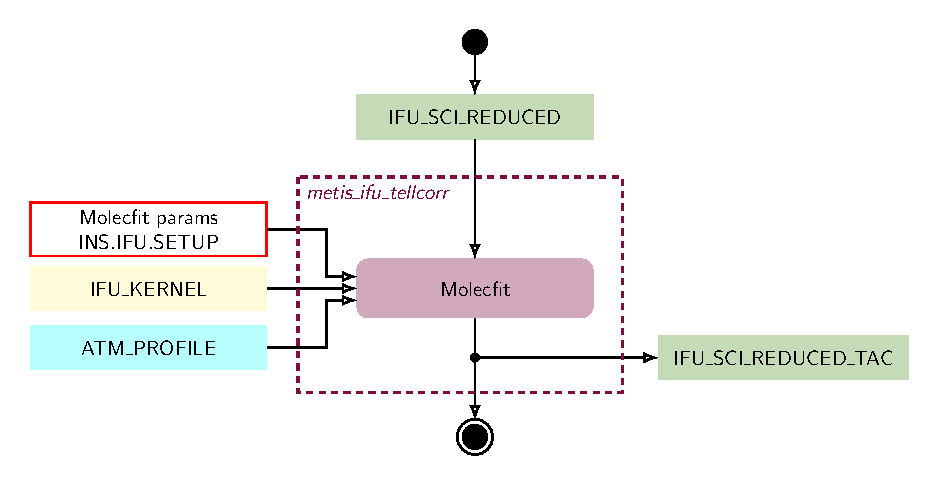
\includegraphics[width=0.7\textwidth]{metis_ifu_tellcorr}
  \caption[Recipe: \REC{metis_ifu_tellcorr}]{\REC{metis_ifu_tellcorr}
    -- telluric correction of reduced IFU science cubes.}
  \label{fig:metis_ifu_tellcorr}
\end{figure}


\clearpage
\subsubsection{IFU science postprocessing}
\label{sssec:ifu_sci_postprocess}
\label{rec:metis_ifu_sci_postprocess}

This recipe combines a number of reduced IFU exposures covering a
different spatial and wavelength ranges into a single data cube. The
positions and orientations of the exposures may differ as follows: \TODO{Reference to operational concept}
\begin{description}
\item[Spatial dithering:] The target is placed at different positions
  along and across the slice. Along-slice dithering aids in background
  subtraction, across-slice dithering is necessary image
  reconstruction given that the slice width undersamples the PSF.
\item[Field rotation:] The field is rotated by 90 degrees between
  exposures. The cube of a single exposure has different pixel scales
  along and across the slice. The goal of combining exposures at
  different rotation angles is to reconstruct images on a square grid
  with pixel scale given by the detector scale (8.2\,mas). The exact
  procedure remains to be investigated; one of the major challenges is
  to find the exact centre of rotation
  (Sect.~8.9 of \cite{DRLS}).
\item[Spectral dithering:] Sequences of exposures are taken at various
  echelle angles in order to cover an increased contiguous wavelength
  range. In the extended mode, such a sequence may cover the
  wavelength gaps between echelle order coverage.
\end{description}

In order to allow co-addition of data from separate OBs, possibly taken
months apart, the wavelengths will be corrected to the heliocentric
reference system before co-addition.

The recipe is only used in the science-grade pipelines, not at the
observatory.

\begin{recipedef}
  Name:           & \hyperref[rec:metis_ifu_sci_postprocess]{\REC{metis_ifu_sci_postprocess}}                                            \\
  Purpose:        & Coaddition and mosaicing of reduced science cubes.                         \\
  Requirements:   & \REQ{METIS-6131}                                                           \\
  Type:           & Science                                                                    \\
  Templates:      & ---                                                                        \\
  Input data:     & Reduced science cubes (\PROD{IFU_SCI_REDUCED}, \hyperref[dataitem:ifu_sci_reduced_tac]{\PROD{IFU_SCI_REDUCED_TAC}}) \\
  Parameters:     & TBD                                                                        \\
  Algorithm:      & Determine cubic output grid encompassing all input cubes                   \\
                  & Resample input cubes to output grid                                        \\
                  & Coadd                                                                      \\
  Output data:    & \hyperref[dataitem:ifu_sci_coadd]{\PROD{IFU_SCI_COADD}}                                                       \\
                  & \hyperref[dataitem:ifu_sci_coadd_error]{\PROD{IFU_SCI_COADD_ERROR}}                                                 \\
  QC1 parameters: & ---                                                                        \\
\end{recipedef}

\begin{figure}[hb]
  \centering
  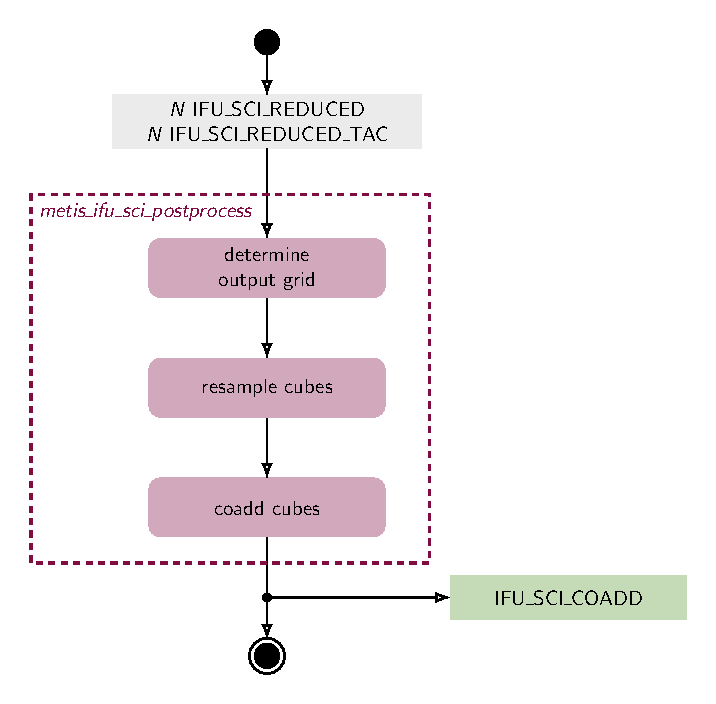
\includegraphics[width=0.7\textwidth]{metis_ifu_sci_postprocess}
  \caption[Recipe: \REC{metis_ifu_sci_postprocess}]{%
    \hyperref[rec:metis_ifu_sci_postprocess]{\REC{metis_ifu_sci_postprocess}} -- post-processing (coaddition) of
    reduced IFU science frames.}
  \label{fig:metis_ifu_sci_postprocess}
\end{figure}


\clearpage
\subsubsection{IFU distortion calibration}
\label{sssec:ifu_distortion}
\label{rec:metis_ifu_distortion}

Calibration of the geometric distortion of the IFU is done by
observing a pin hole mask located in a focal plane within the
instrument. The distortion is described in terms of a polynomial model
whose coefficients can be used to map positions in in the detector
array to sky positions. Measurement of the FWHM of the spots gives an
indication of the variation of spectral resolution across the field of view.

\begin{recipedef}
  Name:                & \hyperref[rec:metis_ifu_distortion]{\REC{metis_ifu_distortion}}                                                  \\
  Purpose:             & Determine geometric distortion coefficients for the IFU.                    \\
  Requirements:        & \REQ{METIS-6087}, \REQ{METIS-6073}                                          \\
  Type:                & Calibration                                                                 \\
  Templates:           & \TPL{METIS_ifu_cal_distortion}                                              \\
  Input data:          & Images of multi-pinhole mask.                                               \\
  Parameters:          & TBD                                                                         \\
  Algorithm:           & Calculate table mapping pixel position to position on sky.                  \\
  Output data:         & \hyperref[dataitem:ifu_distortion_table]{\PROD{IFU_DISTORTION_TABLE}}                                                 \\
                       & \hyperref[dataitem:ifu_dist_reduced]{\PROD{IFU_DIST_REDUCED}}                                                     \\
  Expected accuracies: & TBD                                                                         \\
  QC1 parameters:      & \QC{QC IFU DISTORT RMS}: RMS deviation between measured position and model \\
                       & \QC{QC IFU DISTORT FWHM}:   Measured FWHM of spots                            \\
                       & \QC{QC IFU DISTORT NSPOTS}: Number of identified spots                        \\
\end{recipedef}

\begin{figure}[hb]
  \centering
  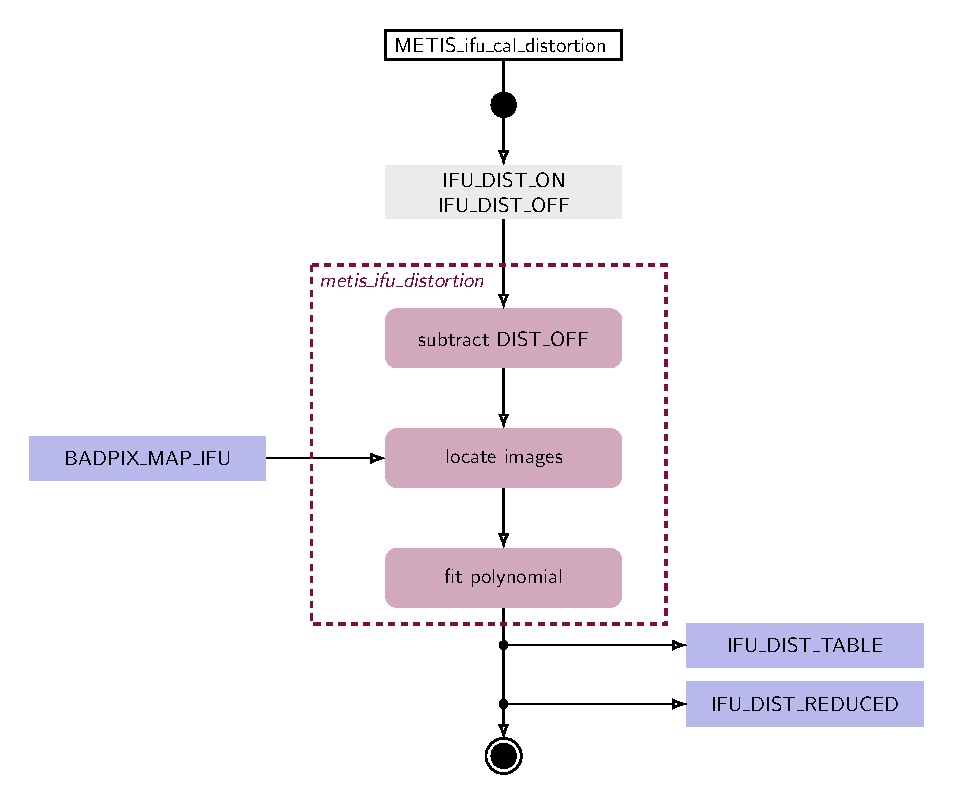
\includegraphics[width=0.6\textwidth]{metis_ifu_distortion}
  \caption[Recipe: \REC{metis_ifu_distortion}]{%
    \hyperref[rec:metis_ifu_distortion]{\REC{metis_ifu_distortion}} -- IFU distortion calibration}
  \label{fig:metis_ifu_distortion}
\end{figure}


\clearpage



%%%%%%%%%%%%%%%%%%%%%%%%%%%%%%%%%%%%%%%%%%%%%%%%%%%%%%%%%%%%%%%%%%%%%%%%%%%%%%%%

%%% Local Variables:
%%% TeX-master: "METIS_DRLD"
%%% End:


\subsection{ADI Post Processing}
\label{}



The following recipes can be used by astronomers in an offline way
perform basic ADI processing on data which have already undergone
basic calibration, via the standard LM/N processing methods.  As it
relies on reduced data they will not be executed in a scheduled way at
the telescope. For more detailed HCI reductions the observers will
have to rely on their own more specialized code, but intermediate data
products will be optionally provided in these recipes to facilitate
their dedicated HCI reductions. Potentially these three recipes can be combined into one with a logical decision tree. To minimize interpolation artefacts any interpolation steps are to be combined as much as possible. Bad pixel maps and image stacks without background subtraction are available as output from the earlier science processing recipes.

\subsubsection{IMG\_LM/N RAVC/CVC(/CLC) ADI Post Processing}
\label{}


The following recipe is applicable for ADI post processing for the LM
and N band, and CVC/RAVC(/CLC) coronagraphs. An input set of
observations consists of a time sequence of ADI images in LM or N band, which have already undergone basic calibration.

For each image, the centroid of the central source is determined, distortion corrections are performed, and the images are aligned on a subpixel scale. The median PSF is then estimated and subtracted from all images following the first step of the standard ADI technique of Marois et al (2006). 
Each image is then derotated using the known position angle and coadded to produce the final science image. In addition, the images prior to PSF subtraction are derotated and combined to produce a second final image.

In addition to the final images, the cube of derotated, PSF subtracted images are used to calculate the raw and post-ADI contrast curves as well as the ADI throughput curve. The intrinsic radial throughput of the coronagraph  is taken from static calibrations while the post-processing losses are estimated from injection and retrieval of artificial companions with a known brightness and separation.

Off-axis unsaturated PSFs which are needed for the ADI process are either collected as part of the observations, static calibrations or available from the QACITS control loop.  If collected as part of the OB they are processed by the regular science recipes (with compensation of any neutral density transmission).

While not part of the PIP specs, the current generation of VIP\_HCI ADI reduction algorithms supports the more detailed Marois et al. 2006 ADI (including an annular optimization step) as well as PCA-based routines.

\begin{recipedef}
  Name:                & \REC{metis_lm_adi_ravc}                                        \\
  Purpose:             & Classical ADI post processing for CVC/RAVC(/CLC) coronagraphs      \\
  Requirements:        & \REQ{METIS-5989}                                               \\
  Type:                & Science                                                    \\
  Templates:           & \TPL{LM_SCI_Reduced}                            \\
  Input data:          & Time series of LM\_SCI\_REDUCED images                      \\
                       & LM distortion table                               \\
                       & Coronagraphic throughput map and profile                                                  \\
                       & Off-axis PSF references                                                  \\
                       &                                                  \\
   Matched keywords:   &              \\
                       &               \\
                       &               \\
                       &               \\
                       &               \\
  Recipe parameters:   &  combination approach (median,mean,sigclip) \\
                       &   combination parameters (e.g., N-sigma)          \\
                       &  start and end limit to contrast curve (in $\lambda/D$) \\
  & frame exclusion thresholds dependent on AO parameters and centroid offset                \\
  
  Algorithm:           & Determine centroid of central source \\
                       & Distortion correction and sub-pixel alignment   \\
                       & Estimate median PSF   \\
                       & Subtract median PSF   \\
                       & De-rotate images   \\
                       & Coadd images   \\
  & Calculate contrast curve   \\
  Output data:       & \PROD{LM_RAVC_SCI_CALIBRATED} (Calibrated Image)                                    \\
                     & \PROD{LM_RAVC_SCI_CENTRED} (Cube of individually calibrated and recentered images)                                 \\
                     & \PROD{LM_RAVC_CENTROID_TAB} (Table of star centre estimages)                                 \\
              
                     & \PROD{LM_RAVC_SCI_SPECKLE} (PSF/speckle image)                                 \\
                     & \PROD{LM_RAVC_SCI_DEROTATED_PSFSUB_COADD} (Combined derotated image with PSF subtraction)                                 \\
                     & \PROD{LM_RAVC_SCI_DEROTATED_COADD} (Combined derotated image without PSF subtraction)                                  \\
                     & \PROD{LM_RAVC_SCI_CONTRAST_RAW} (Raw Contrast Curve)                                 \\
                     & \PROD{LM_RAVC_SCI_CONTRAST_ADI} (Post ADI Contrast Curve)                                 \\
                     & \PROD{LM_RAVC_SCI_THROUGHPUT} (ADI Throughput Curve)                               \\
                     & \PROD{LM_RAVC_SCI_COVERAGEMAP} (ADI Coverage Map: number of frames  
                     \\
                     & \PROD{LM_RAVC_SCI_SNR} (ADI SNR Map)  \\

  Expected accuracies: & \TBD                                                           \\
  QC1 parameters:      & \QC{FWHM of PSF by frame}                                      \\
                       & \QC{Raw and post ADI contrast at seps (1,2,5,10,20,40 lam/D)}                                        \\
                       & \QC{Mean SNR in ADI map}                                        \\
                       & \QC{Peak SNR in ADI map}                                         \\
  hdrl function        & \CODE{}                                    \\
                       & \CODE{}                                 \\
                       & \CODE{}                                \\
\end{recipedef}

\begin{figure}[hb]
  \centering
  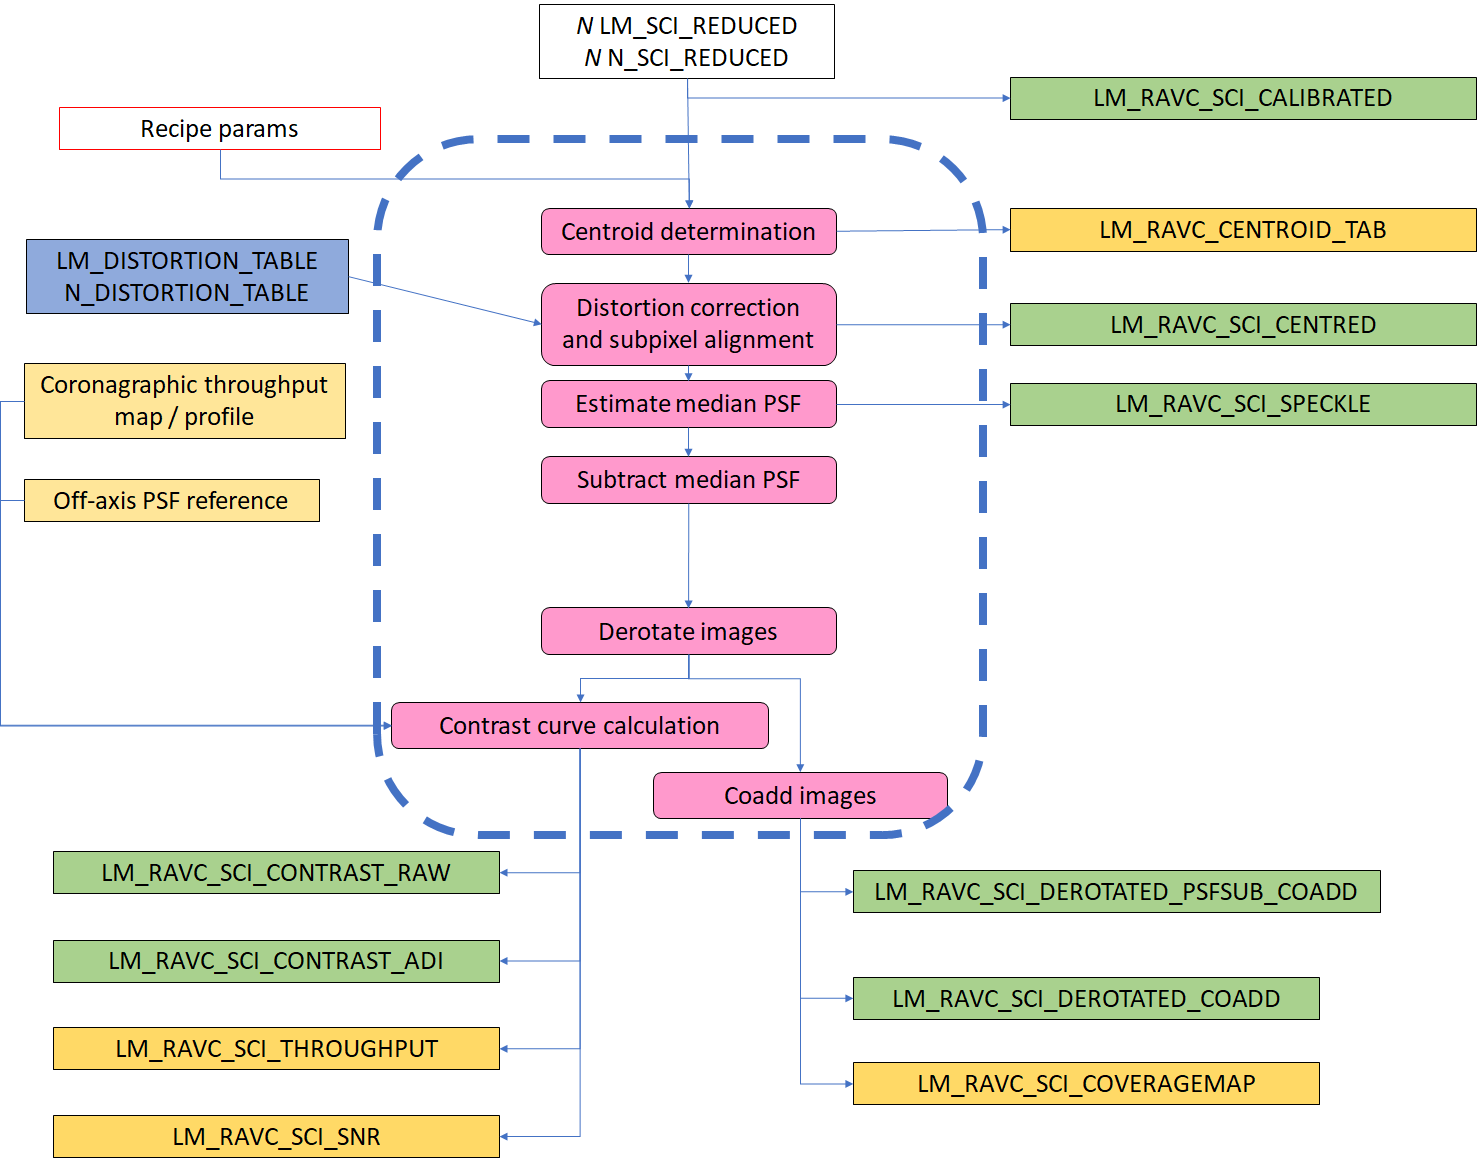
\includegraphics[width=0.6\textwidth]{./figures/metis_lm_adi_ravc}
  \caption[Recipe: \REC{metis_lm_adi_ravc}]{\REC{metis_lm_adi_ravc} -- LM ADI post processing for RAVC/CVC(/CLC) coronagraph. 
    }
  \label{fig:metis_lm_adi_ravc}
\end{figure}




\subsubsection{IMG\_LM/N APP ADI Post Processing}
\label{}


The following recipe is applicable for ADI post processing for the LM and N band, in combination with the APP coronagraph. It is very similar to the recipe for RAVC/CVC(/CLC) coronagraphs, with the addition of steps to merging together the two half PSFs, and of applying an angular wedge mask before the derotation and stacking, and contrast curve calculations. An input set of observations consists of a time sequence of ADI images in LM/N band, which have already undergone basic calibration.

For each image, the centroid of the central source is determined for all three PSFs and distortion corrections are performed. The PSFs are aligned at a sub-pixel scale and extracted; the extracted coronagraphic PSFs are merged to produce a complete PSF and the third PSF is used to form a cube of calibrated leakage PSFs.
The mean/median/sigmaclipped PSF is estimated and subtracted from each frame of the merged coronagraphic PSF. Each image is
then derotated to place the off-axis source at the same on-sky angle and coadded to produce the final stacked science image. In addition, the images prior to PSF subtraction are derotated and combined to produce a second final stacked image.

In addition to the final images, the stack of derotated, PSF subtracted images are used to calculate the raw and post-ADI contrast curves as well as the ADI throughput curve and coverage map containing the effective number of included frames.



\begin{recipedef}
  Name:                & \REC{metis_lm_adi_app}                                        \\
  Purpose:             & Classical ADI post processing for APP coronagraph      \\
  Requirements:        & \REQ{METIS-5989}                                               \\
  Type:                & Science                                                    \\
  Templates:           & \TPL{LM_SCI_Reduced}                            \\
  Input data:          & Time series of LM\_SCI\_REDUCED images                      \\
                       & LM distortion table                               \\
                       & Off-axis PSF reference                                                  \\
                       &                                                  \\
   Matched keywords:   &              \\
                       &               \\
                       &               \\
                       &               \\
                       &               \\
  Recipe parameters:   &  combination approach (median,mean,sigclip) \\
                       &   combination parameters (e.g., N-sigma)          \\
                       &  start and end limit to contrast curve (in $\lambda/D$) \\
  & frame exclusion thresholds dependent on AO parameters and centroid offset \\
                                                       
  Algorithm:           & Determine centroid of central source \\
                       & Distortion correction and sub-pixel alignment   \\
                       & sub-pixel PSF extraction and alignment   \\
                       & Merge coronagraphic PSFs   \\
                       & Estimate median PSF   \\
                       & Subtract median PSF   \\
                       & De-rotate images   \\
                       & Coadd images   \\
                       & Calculate contrast curves   \\
  & Calculate contrast curve   \\
  Output data:       & \PROD{LM_APP_SCI_CALIBRATED} (Calibrated Image)                                    \\
                     & \PROD{LM_APP_SCI_CENTRED} (Cube of individually calibrated and recentered images)                                 \\
                     & \PROD{LM_APP_CENTROID_TAB} (Table of star centre estimates)                                 \\
              
                     & \PROD{LM_APP_SCI_SPECKLE} (PSF/speckle image)                                 \\
                     & \PROD{LM_APP_SCI_DEROTATED_PSFSUB} (Combined derotated image with PSF subtraction)                                 \\
                     & \PROD{LM_APP_SCI_DEROTATED_COADD} (Combined derotated image without PSF subtraction)                                  \\
                     & \PROD{LM_APP_SCI_CONTRAST_RAW} (Raw Contrast Curve)                                 \\
                     & \PROD{LM_APP_SCI_CONTRAST_ADI} (Post ADI Contrast Curve)                                 \\
                     & \PROD{LM_APP_SCI_THROUGHPUT} (ADI Throughput Curve)                               \\
                     
                     & \PROD{LM_APP_SCI_COVERAGEMAP} (ADI Coverage Map: number of frames
                     \\
                     & \PROD{LM_APP_SCI_SNR} (ADI SNR Map)                            \\

  Expected accuracies: & \TBD                                                           \\
  QC1 parameters:      & \QC{FWHM of PSF by frame}                                      \\
                       & \QC{Raw and post ADI contrast at seps (1,2,5,10,20,40 lam/D)}                                        \\
                       & \QC{Mean SNR in ADI map}                                        \\
                       & \QC{Peak SNR in ADI map}                                         \\
  hdrl function        & \CODE{}                                    \\
                       & \CODE{}                                 \\
                       & \CODE{}                                \\
\end{recipedef}

\begin{figure}[hb]
  \centering
  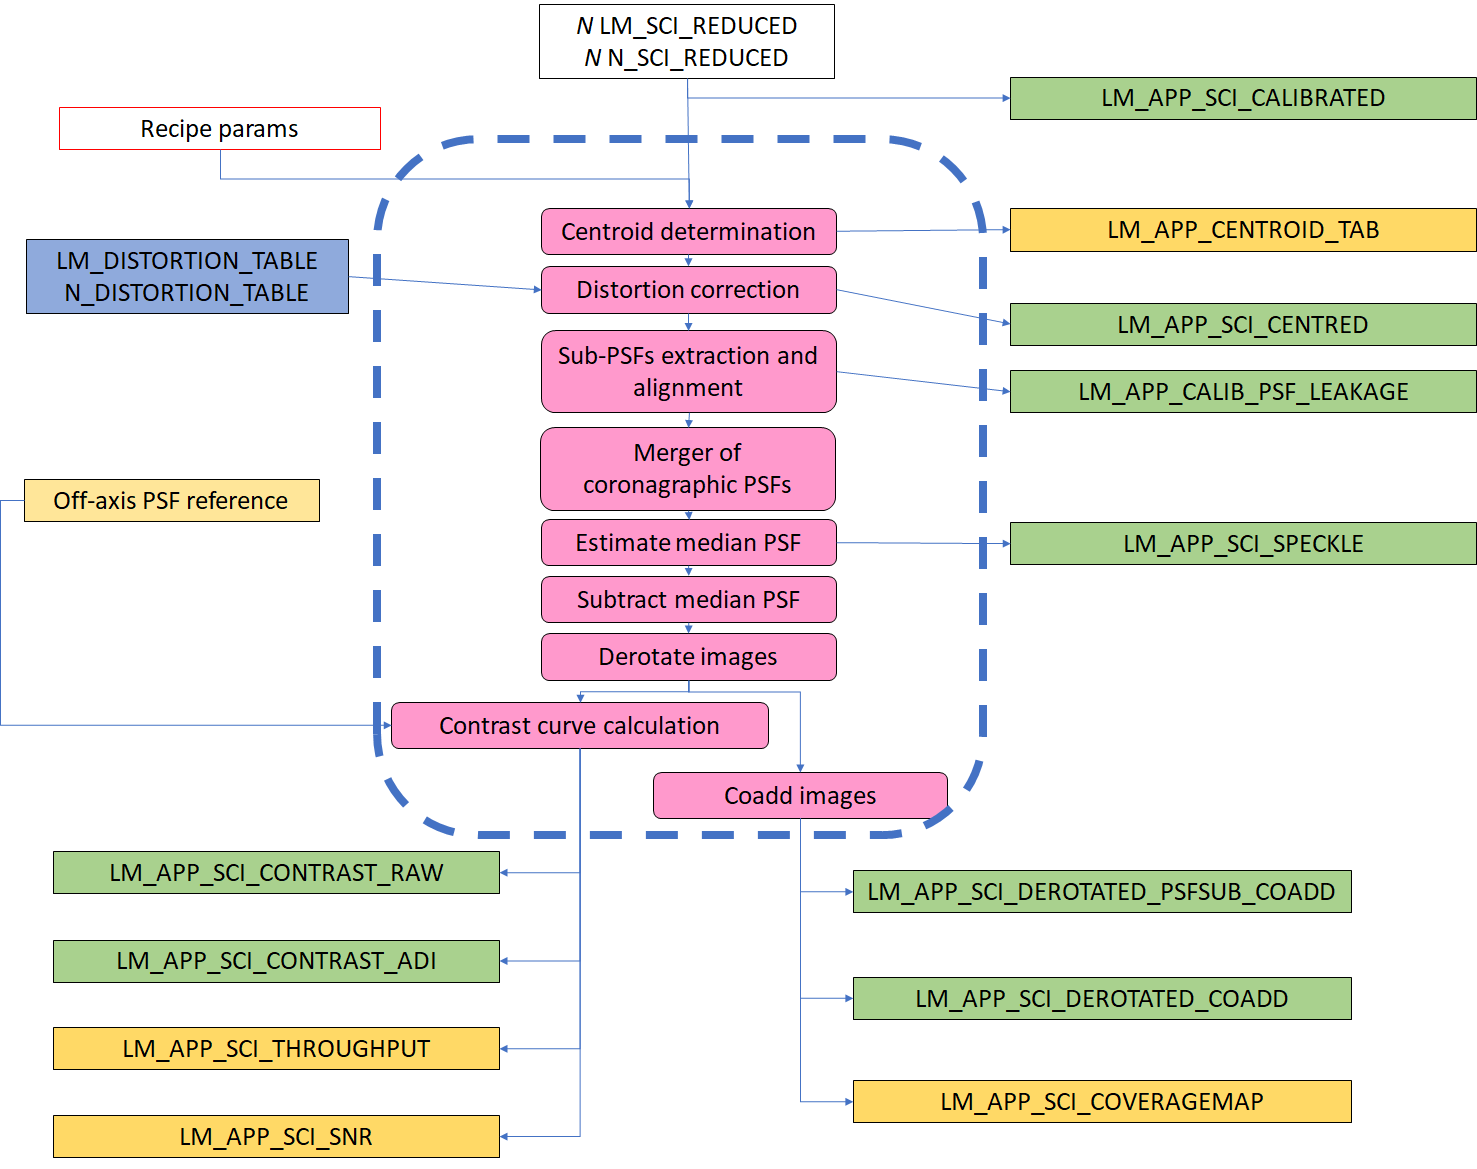
\includegraphics[width=0.6\textwidth]{./figures/metis_lm_adi_app}
  \caption[Recipe: \REC{metis_lm_adi_app}]{\REC{metis_lm_adi_app} -- LM ADI post processing for APP coronagraph. 
    }
  \label{fig:metis_lm_adi_app}
\end{figure}



\subsubsection{LMS ADI Post Processing}
\label{}


The following recipe is applicable for ADI post processing for the LMS data cubes and the RAVC/CVC and APP coronagraphs. As only a single target can be targeted in the limited field of view the methods overlap between coronagraphs.
For the LMS observations, the input is a set of reduced 3D (spectral and spatial) data cubes on a rectified grid. 

For each wavelength slice in each cube the centroid is determined by a QACITS-like algorithm in the case of the focal plane coronagraphs (RAVC/CVC) or through 2D cross-correlation with a template PSF for the APP coronagraph. This centroid information is stored in a table together with timestamps, parallactic angle and bad frame flags (based on AO loop status, AO performance, atmospheric parameters and centroid offset).
As the ADI step requires square pixels following previous work on combining ADI techniques with IFUs (such as SPHERE/IFS, SINFONI), the rectangular spatial grid is interpolated or nearest neighbor filled to produce a square pixel image. 
It is acknowledged that one spatial dimension is undersampled which may lead to reduced performance.
The mean/median/sigmaclipped PSF (in time) is estimated for each wavelength and subtracted from each image in the cube. 
After derotation the cubes are combined in time to give a coadded cube. For the APP a wedge shape is used. The limited field of view of the LMS means that only PSF can be centered on the IFU. The derotated cubes are also used to generate post ADI contrast curves and contrast curves with input from the radial coronagraph throughput profile and off-axis PSFs. In addition coverage maps are produced.

While not part of the PIP specs, the current generation of VIP\_HCI ADI reduction algorithms supports
the more detailed Marois et al. 2006 ADI routine, PCA-based routines, as well as ADI+mSDI processing to improve the speckle PSF estimation with the additional wavelength information.



\begin{recipedef}
  Name:                & \REC{metis_lms_adi_ravc}                                        \\
  Purpose:             & Classical ADI post processing for APP/CVC/RAVC(/CLC) coronagraphs      \\
  Requirements:        & \REQ{METIS-5989}                                               \\
  Type:                & Science                                                    \\
  Templates:           & \TPL{LMS_SCI_Reduced}                            \\
  Input data:          & Time series of LMS\_SCI\_REDUCED images                      \\
                       & LM distortion table                               \\
                       & Coronagraphic throughput map and profile                                                  \\
                       & Off-axis PSF references                                                  \\
                       &                                                  \\
   Matched keywords:   &              \\
                       &               \\
                       &               \\
                       &               \\
                       &               \\
  Recipe parameters:   &  combination approach (median,mean,sigclip) \\
                       &   combination parameters (e.g., N-sigma)          \\
                       &  start and end limit to contrast curve (in $\lambda/D$) \\
  & frame exclusion thresholds dependent on AO parameters and centroid offset \\
                                                       
  Algorithm:           & Determine centroid of central source \\
                       & Distortion correction, square pixel reconstruction and sub-pixel alignment   \\
                       & Estimate median PSF   \\
                       & Subtract median PSF   \\
                       & Derotate images   \\
                       & Coadd images   \\
                       & Calculate contrast curves   \\
 
  Output data:       & \PROD{LMS_RAVC_SCI_CALIBRATED} (Calibrated Cube)                                    \\
                     & \PROD{LMS_RAVC_SCI_CENTRED} (Cube of individually calibrated and recentered cubes)                                 \\
                     & \PROD{LMS_RAVC_CENTROID_TAB} (Table of star centre estimages)                                 \\
              
                     & \PROD{LMS_RAVC_SCI_SPECKLE} (PSF/speckle cube)                                 \\
                     & \PROD{LMS_RAVC_SCI_DEROTATED_PSFSUB} (Combined derotated cube with PSF subtraction)                                 \\
                     & \PROD{LMS_RAVC_SCI_DEROTATED_COADD} (Combined derotated cube without PSF subtraction)                                  \\
                     & \PROD{LMS_RAVC_SCI_CONTRAST_RAW} (Raw Contrast Curves)                                 \\
                     & \PROD{LMS_RAVC_SCI_CONTRAST_ADI} (Post ADI Contrast Curves)                                 \\
                     & \PROD{LMS_RAVC_SCI_THROUGHPUT} (ADI Throughput Curves)                               \\
                     & \PROD{LMS_RAVC_SCI_SNR} (ADI SNR Map)                            \\

  Expected accuracies: & \TBD                                                           \\
  QC1 parameters:      & \QC{FWHM of PSF by frame}                                      \\
                       & \QC{Raw and post ADI contrast at seps (1,2,5,10,20,40 lam/D)}                                        \\
                       & \QC{Mean SNR in ADI map}                                        \\
                       & \QC{Peak SNR in ADI map}                                         \\
  hdrl function        & \CODE{}                                    \\
                       & \CODE{}                                 \\
                       & \CODE{}                                \\
\end{recipedef}

\begin{figure}[hb]
  \centering
  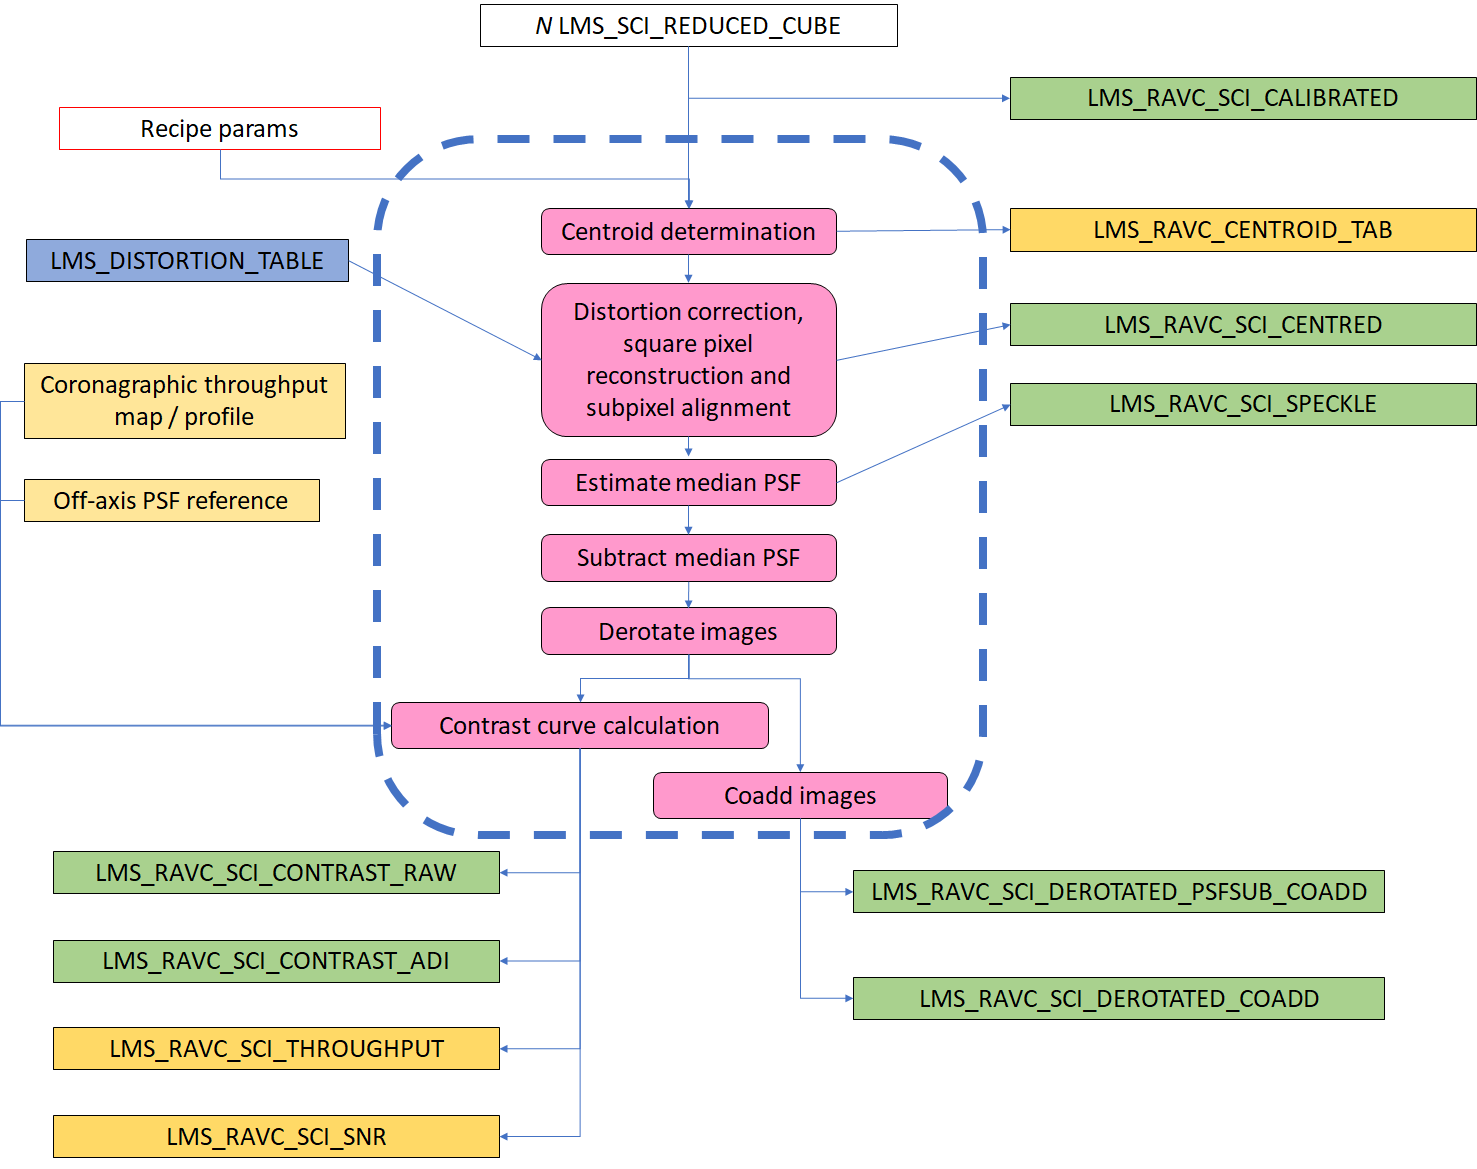
\includegraphics[width=0.6\textwidth]{./figures/metis_lms_adi_ravc}
  \caption[Recipe: \REC{metis_lms_adi_ravc}]{\REC{metis_lms_adi_ravc} -- LMS ADI post processing for RAVC coronagraph. 
    }
  \label{fig:metis_lms_adi_ravc}
\end{figure}

 
\subsection{Recipes for engineering templates}
\label{ssec:recipes_technical}

% HB 20230726: We decided that the recipes listed here should be included.
%\TBD It is not clear (2020-11-19) whether data from maintenance
%templates need to be reduced by the pipeline. This section and the
%recipes described therein serves as a placeholder and may be removed
%later.

The CLC coronagraph was removed from the baseline coronagraphic modes before FDR however the coronagraph would be technically available during engineering. At this stage the DRL will not have the corresponding recipes to use the CLC. However, if the need arises during commissioning or after to make the CLC mode available, its DRL recipe can be easily adapted from the baseline RAVC/CVC coronagraph recipes as it is related in design and usage.

%------------------------------------------------------------------------------------------------------------------
\subsubsection{\REC*{metis_pupil_imaging}: Pupil imaging}\label{rec:metis_pupil_imaging}
\label{sssec:pupil_imaging}

This recipe refers to pupil imaging using the science detectors.
Pupil imaging is needed to verify the alignment and illumination of the pupil masks (part of the HCI coronagraphs) with the telescope beam.
It is not foreseen to be used by scientists in regular operation.

% From OC:
%Presumably it only contains the most basic reduction  steps.
%There may have to be separate recipes for the various
%subsystems.

% From GO:
%Also it can be used to record the pupil transmission which can improve PSF modelling.
%A simple reduction to get rid of bias effects might be enough to align the pupil, and it might already be possible on the raw data.
%If they want pupil transmission they likely also expect some pixel response or flatfield correction.

\begin{recipedef}
  Name                 & \REC{metis_pupil_imaging}                     \\
  Purpose:             & Apply basic reduction to pupil imaging data.  \\
  Requirements:        & --                                            \\
  Type:                & Maintenance                                   \\
  Templates:           & \TPL{METIS_pup_lm}                            \\
                       & \TPL{METIS_pup_n}                             \\
  Input data:          & \RAW{LM_PUPIL_RAW} or \RAW{N_PUPIL_RAW}       \\
                       & \PROD{GAIN_MAP_2RG} or \PROD{GAIN_MAP_GEO}    \\
  Matched keywords:    & \FITS{DRS.PUPIL}                              \\
  Algorithm            & Apply dark current and flat field corrections.\\
  Output data:         & \PROD{LM_PUPIL_REDUCED} or \PROD{N_PUPIL_REDUCED} \\
  Expected accuracies: & n/a                                           \\
  QC1 parameters:      & None                                          \\
\end{recipedef}

\clearpage
%------------------------------------------------------------------------------------------------------------------
\clearpage
\subsubsection{\REC*{metis_img_chophome}: Chopper Home Position recipe }\label{ssec:metisimgchophome}
The recipe \REC{metis_img_chophome} aims to detect chopper mirror zero positions. Currently it is foreseen on daily basis to be carried out, but is for sure necessary after switching on the chopper (e.g. after instrument interventions) or induced by unforeseen events like earthquakes (cf. Section "Chopper Home Position" in  \cite{METIS-calibration_plan}).

The procedure consists of measuring the position of a point source from the \ac{WCU}, that has been centred on the \ac{WFS} pyramid (in the K-band), in the \CODE{IMG_LM} mode.
Then, taking the respective positional metrology values of the \ac{WFS}-FS and the chopper,
% TODO: What is the FS in WFS-FS?
the relative coordinates between the \ac{WFS} Pyramid focal plane, and the science focal planes is established.
%  (the latter in plural because we have already calibrated the relative astrometry between between IMG-LM and IMG-N/LMS).

\begin{figure}[ht]
  \centering
  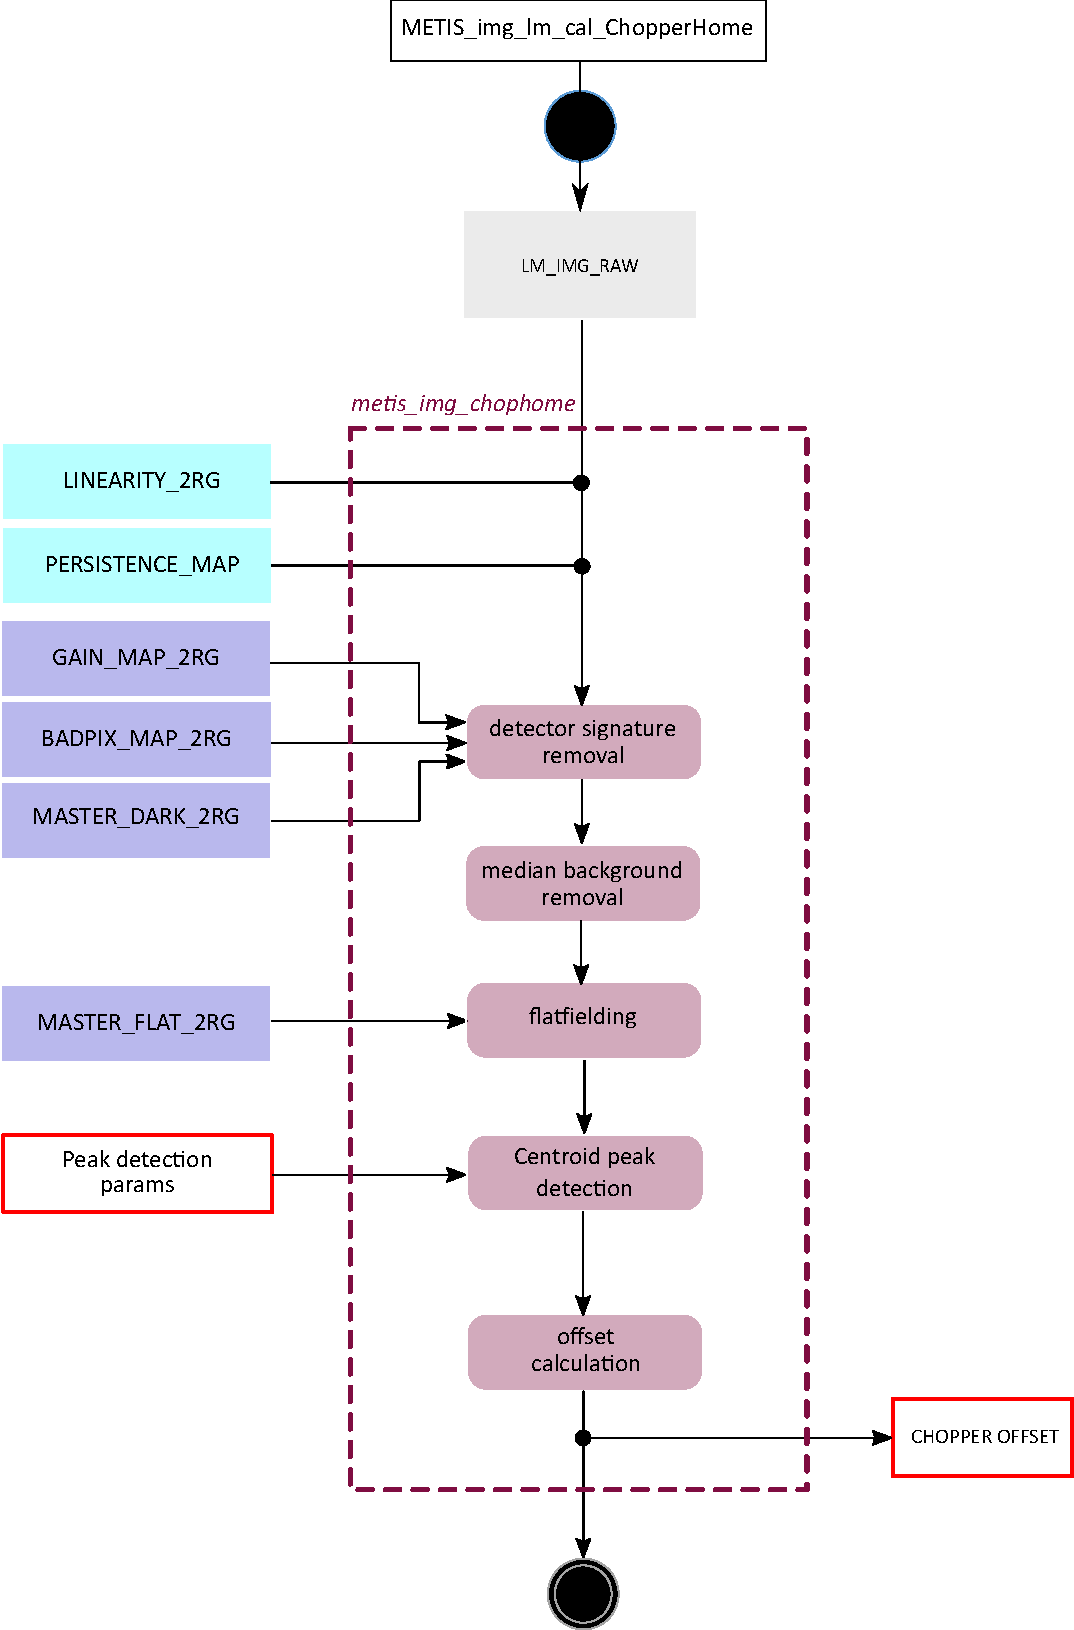
\includegraphics[width=0.5\textheight]{figures/metis_img_chophome_v0.83.pdf}
  \caption[Recipe: \REC*{metis_img_chophome}]{\REC*{metis_img_chophome} --
    Recipe workflow to detect the zero position of the chopper mirror.}
  \label{Fig:rec_chop_home}
\end{figure}

\begin{recipedef}\label{rec:metisimgchophome}\label{rec:metis_img_chophome}
Name:		& \REC{metis_img_chophome} \\
Purpose:	& Detection of the chopper mirror home position \\
Type:		& Calibration\\
Requirements: & None \\
Templates:      & \TPL{METIS_img_lm_cal_ChopperHome} \\
Input data:     & \RAW{LM_CHOPPERHOME_RAW} \\
                & \EXTCALIB{PERSISTENCE_MAP}  \\
                & \STATCALIB{LINEARITY_2RG}  \\
                & \PROD{GAIN_MAP_2RG}  \\
%                & \PROD{BADPIX_MAP_2RG}  \\
                & \PROD{MASTER_DARK_2RG}  \\
                & \PROD{MASTER_IMG_FLAT_LAMP_LM}  \\
Matched Keywords & \FITS{DET.DIT} \\
                 & \FITS{DET.NDIT} \\
                 & \FITS{DRS.FILTER} \\
Parameters: 	& None\\
Algorithm:      & remove detector signature\\
                & remove median background\\
                & apply flatfield\\
                & detect reference source from \ac{WCU} via centroid peak detection\\
                & Calculate mirror offset\\
Output data:	& Offset of the chopper mirror to be piped either into the \ac{ICS} for correction \\
                & or to be used in thee pipeline for astrometric correction\\
Expected accuracies: & 0.1mas accuracy of the centroid position (cf.~\cite{METIS-calibration_plan})\\
QC1 parameters: & None\\
\end{recipedef}
\clearpage

%------------------------------------------------------------------------------------------------------------------
% Moved to https://github.com/AstarVienna/METIS_DRLD/issues/101
% \subsubsection{Plate-scale calibration}
% \TODO{Plate-scale calibration}

%------------------------------------------------------------------------------------------------------------------
\clearpage
\subsubsection{\REC*{metis_lm_adc_slitloss} and \REC*{metis_n_adc_slitloss}: Slit loss determination }\label{sssec:adc_slitlosses}
The recipes \REC{metis_lm_adc_slitloss} (Fig.~\ref{Fig:rec_lm_adc_slitloss}) and \REC{metis_n_adc_slitloss} (Fig.~\ref{Fig:rec_n_adc_slitloss}) aims to determine the throughput as function of the object position along the across-slit direction. It is expected that the usage of the fixed positioned \ac{ADC} will introduce flux losses (cf. Section "Calibration of slit losses" in  \cite{METIS-calibration_plan}). For the determination, the point sources (i.e. mask of the \ac{WCU}) is placed on several positions (distance $\sim\frac{1}{10}\lambda/D$) across the slit (cf. Fig.~\ref{Fig:slitloss}), and measure the wavelength dependent flux changes with respect to the respective positions. Finally, a simple model is determined to be able to correct for the flux losses  (see Section "Calibration of slit losses" in the Calibration Plan~\cite{METIS-calibration_plan} for more details). This recipe is to be carried out once in a while to update the static calibration database.
\begin{figure}[ht]
  \centering
  
\includegraphics[width=0.5\textheight]{figures/slitloss_det.pdf}
  \caption[slitloss determination]{Algorithm for the slit-loss determination in recipe \REC{metis_lm_adc_slitloss} }
  \label{Fig:slitloss}
\end{figure}

\begin{figure}[ht]
  \centering
  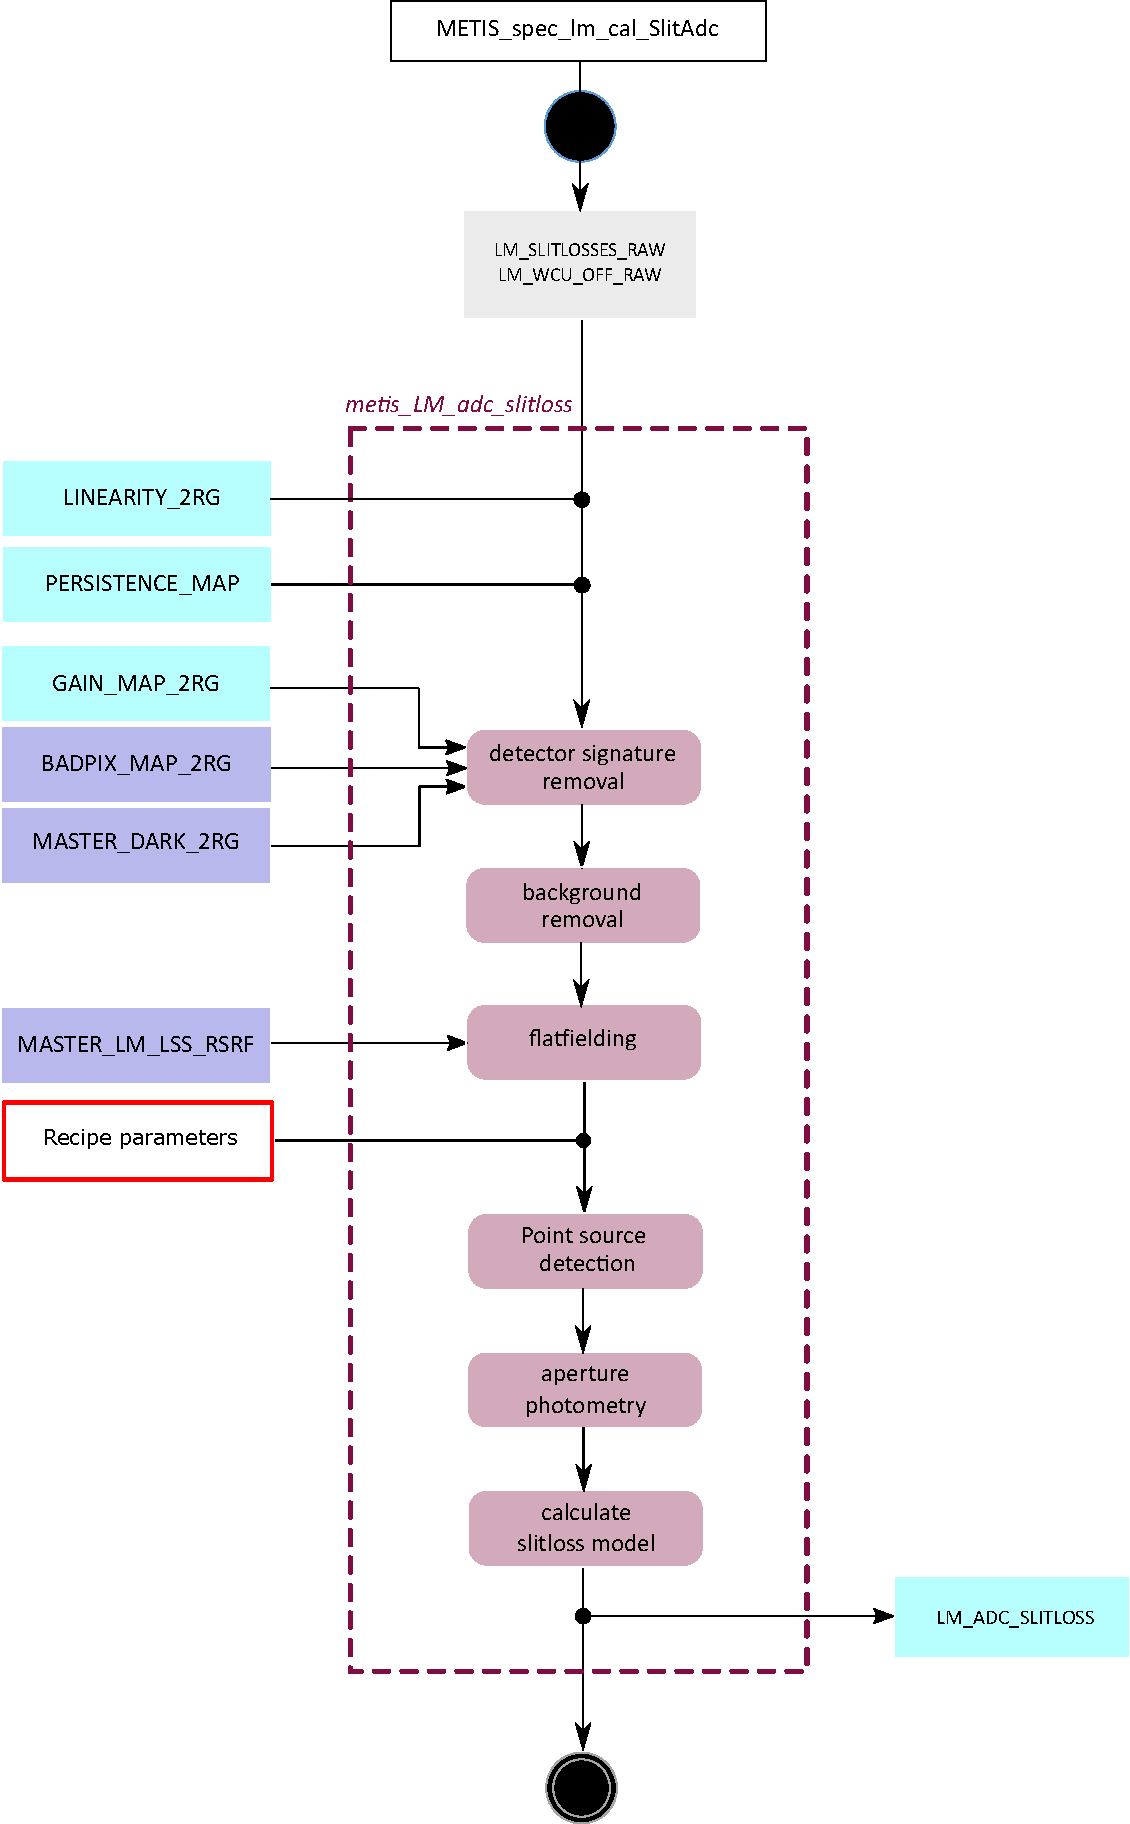
\includegraphics[width=0.5\textheight]{figures/metis_lm_adc_slitloss_v0.83.pdf}
  \caption[Recipe: \REC*{metis_lm_adc_slitloss}]{\REC*{metis_lm_adc_slitloss} --
    Recipe workflow to determine the \ac{ADC} induced slit losses.}
  \label{Fig:rec_lm_adc_slitloss}
\end{figure}

\begin{recipedef}\label{rec:metislmadcmslitloss}\label{rec:metis_lm_adc_slitloss}
Name:		& \REC{metis_lm_adc_slitloss} \\
Purpose:	& Determination of the \ac{ADC} induced slit losses \\
Type:		& Calibration\\
Requirements: &  METIS-6074, METIS-2757, METIS-9099, METIS-9150\\
Templates:           & \TPL{METIS_spec_lm_cal_SlitAdc} \\
Input data:     & \RAW{LM_SLITLOSSES_RAW} \\
                & \RAW{LM_WCU_OFF_RAW} \\
                & \EXTCALIB{PERSISTENCE_MAP}  \\
                & \STATCALIB{LINEARITY_2RG}  \\
                & \PROD{GAIN_MAP_2RG}  \\
                & \PROD{BADPIX_MAP_2RG}  \\
                & \PROD{MASTER_DARK_2RG}  \\
                & \PROD{MASTER_IMG_FLAT_LAMP_LM}  \\
Matched Keywords & \FITS{DET.DIT} \\
                 & \FITS{DET.NDIT} \\
                 & \FITS{DRS.FILTER} \\
Parameters: 	& exposure time, offset positions\\
Algorithm:      & remove detector signature\\
                & remove dark\\
                & apply flatfield\\
                & detect reference source from \ac{WCU} via centroid peak detection\\
                & apply aperture photometry\\
                & calculate (simple) slitloss model (details to be defined)\\
Output data:	& \STATCALIB{LM_ADC_SLITLOSS} (Slit loss model as function of the wavelength and object position across the slit \\
Expected accuracies: & 3\% (cf.~\cite{METIS_calerrbudget})\\
%QC1 parameters: & \QC*{TBD}: TBD\\
\end{recipedef}


\begin{figure}[ht]
  \centering
  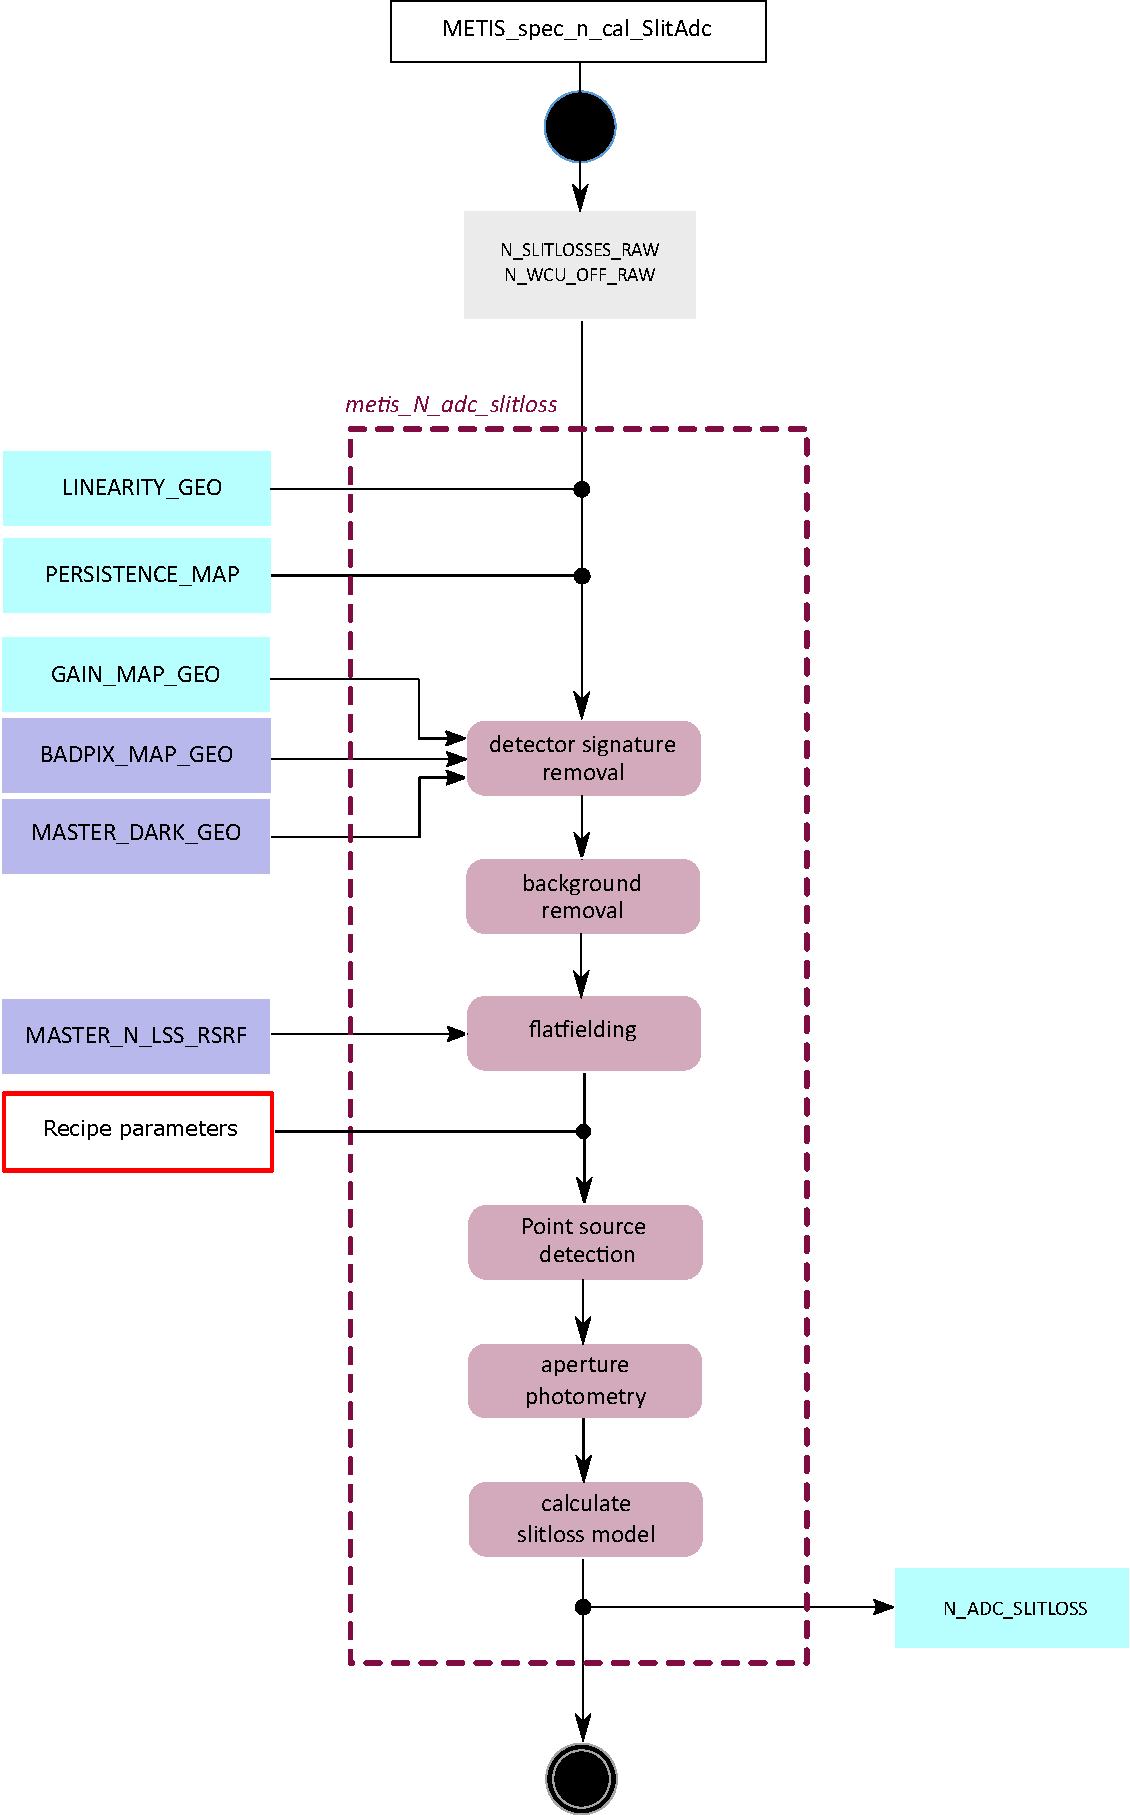
\includegraphics[width=0.5\textheight]{figures/metis_n_adc_slitloss_v0.83.pdf}
  \caption[Recipe: \REC*{metis_n_adc_slitloss}]{\REC*{metis_n_adc_slitloss} --
    Recipe workflow to determine the \ac{ADC} induced slit losses.}
  \label{Fig:rec_n_adc_slitloss}
\end{figure}

\begin{recipedef}\label{rec:metisnadcmslitloss}\label{rec:metis_n_adc_slitloss}
Name:		& \REC{metis_n_adc_slitloss} \\
Purpose:	& Determination of the \ac{ADC} induced slit losses \\
Type:		& Calibration\\
Requirements: & METIS-6074, METIS-2757, METIS-9099, METIS-9150 \\
Input data:     & \RAW{N_SLITLOSSES_RAW} \\
                & \RAW{N_WCU_OFF_RAW} \\
                & \EXTCALIB{PERSISTENCE_MAP}  \\
                & \STATCALIB{LINEARITY_GEO}  \\
                & \PROD{GAIN_MAP_GEO}  \\
                & \PROD{BADPIX_MAP_GEO}  \\
                & \PROD{MASTER_DARK_GEO}  \\
& \PROD{MASTER_IMG_FLAT_LAMP_N}  \\
Matched Keywords & \FITS{DET.DIT} \\
                 & \FITS{DET.NDIT} \\
                 & \FITS{DRS.FILTER} \\
Parameters: 	& exposure time, offset positions\\
Algorithm:      & remove detector signature\\
                & remove dark\\
                & apply flatfield\\
                & detect reference source from \ac{WCU} via centroid peak detection\\
                & apply aperture photometry\\
                & calculate (simple) slitloss model (details to be defined)\\
Output data:	& \STATCALIB{N_ADC_SLITLOSS} (Slit loss model as function of the wavelength and object position across the slit) \\
Expected accuracies: & 3\% (cf.~\cite{METIS_calerrbudget})\\\\
%QC1 parameters: & \QC*{TBD}: TBD\\
\end{recipedef}

%------------------------------------------------------------------------------------------------------------------
\subsubsection{Fringing correction}
\label{rec:metis_fringing_correction}

It is unclear for the time being how much of a problem will be with the METIS
detectors, and what the best strategy will be to tackle it. Therefore, the
method to use will be chosen based on AIT results (\REQ{METIS-9151}, for rationale and basic method description see Ch.~3.12 in the Calibration Plan~\cite{METIS-calibration_plan}).

Whether a stand-alone recipe will be required, or if the fringe-map will become
part of another recipe, is part of that uncertainty. If needed, the design of
said recipe will be minimal work and is thus omitted in this document.

%%% Local Variables:
%%% mode: latex
%%% TeX-master: "METIS_DRLD"
%%% End:


%%% Local Variables:
%%% TeX-master: "METIS_DRLD"
%%% End:
